\documentclass{wissdoc}

% Autor: Roland Bless 1996-2009, bless <at> kit.edu
% ----------------------------------------------------------------
% Diplomarbeit - Hauptdokument
% ----------------------------------------------------------------
%%
%% $Id: diplarb.tex 53 2009-12-10 12:23:37Z bless $
%%
% wissdoc Optionen: draft, relaxed, pdf --> siehe wissdoc.cls
% ------------------------------------------------------------------
% Weitere packages: (Dokumentation dazu durch "latex <package>.dtx")
%\usepackage{bibgerm}
\usepackage[backend=biber, style=numeric]{biblatex} 
\usepackage{csquotes} 
\usepackage{tabularx}
\usepackage{booktabs}
\usepackage{svg}
\usepackage{multirow}
%\usepackage{tocbibind}
\usepackage{siunitx}
\usepackage{xcolor}
\usepackage{textcomp}
\usepackage{listings}
\usepackage{newfloat,caption}
\usepackage{subcaption}
\usepackage{footnote}
\usepackage{rotating}
\usepackage{pgfplots}
\usepackage{pgfplotstable}
\usepackage{url}
\usepackage{boxhandler}
\usepackage{pdfpages}
\usepackage{tabu}
\usepackage{amssymb}
%\usepackage{subfig}
%\usepackage{subcaption}
\usepackage{caption}
\usepackage{subcaption}
%\usepackage[plainpages=true]{hyperref}
\usepackage[space]{grffile}
%\usepackage[numbers,sort&compress]{natbib}
% \usepackage[backend=bibtexu,natbib=true,hyperref=true,doi=false,url=false]{biblatex}
% \usepackage{varioref}
% \usepackage{verbatim}
\usepackage{float}    %z.B. \floatstyle{ruled}\restylefloat{figure}
%\usepackage[hidelinks]{hyperref}
% \usepackage{subfigure}
% \usepackage{fancybox} % für schattierte,ovale Boxen etc.
% \usepackage{tabularx} % automatische Spaltenbreite
% \usepackage{supertab} % mehrseitige Tabellen
% \usepackage[svnon,svnfoot]{svnver} % SVN Versionsinformation 

%%%%%%%%%%%%%%%%%%%%%%%%%% OWN PACKAGES %%%%%%%%%%%%%%%%%%%%%%%%%%%%%%%%%
\usepackage{wrapfig}
\usepackage{caption}
\usepackage{subcaption}
%% ---------------- end of usepackages -------------

%\svnversion{$Id: diplarb.tex 53 2009-12-10 12:23:37Z bless $} % In case that you want to include version information in the footer
%\hyphenation{if...-then...}
%% Informationen für die PDF-Datei
\pgfplotsset{compat=newest}

\hypersetup{
%%% styling of link inside pdf
	colorlinks,
  citecolor=black,
  filecolor=black,
  linkcolor=black,
  urlcolor=black,
%%%		
 pdfauthor={FirstName LastName},
 pdftitle={Title of Thesis}
 pdfsubject={Not set},
 pdfkeywords={Not set}
}
\DeclareFloatingEnvironment[fileext=frm,placement={!ht},name=Listing,within=section]{listing}

% Macros, nicht unbedingt notwendig
%%%%%%%%%%%%%%%%%%%%%%%%%%%%%%%%%%%%%%%%%%%%%%%%%%%%%%%%%%
% macros.tex -- einige mehr oder weniger nuetzliche Makros
% Autor: Roland Bless 1998
%%%%%%%%%%%%%%%%%%%%%%%%%%%%%%%%%%%%%%%%%%%%%%%%%%%%%%%%%%
% $Id: macros.tex 33 2007-01-23 09:00:59Z bless $
%%%%%%%%%%%%%%%%%%%%%%%%%%%%%%%%%%%%%%%%%%%%%%%%%%%%%%%%%%


%%%%%%%%%%%%%%%%%%%%%%%
% Kommentare 
%%%%%%%%%%%%%%%%%%%%%%%
\ifnotdraftelse{
\newcommand{\Kommentar}[1]{}
}{\newcommand{\Kommentar}[1]{{\em #1}}}
% Alles innerhalb von \Hide{} oder \ignore{} 
% wird von LaTeX komplett ignoriert (wie ein Kommentar)
\newcommand{\Hide}[1]{}
\let\ignore\Hide

%%%%%%%%%%%%%%%%%%%%%%%%%
% Leere Seite ohne Seitennummer, wird aber gezaehlt
%%%%%%%%%%%%%%%%%%%%%%%%%

\newcommand{\leereseite}{% Leerseite ohne Seitennummer, nächste Seite rechts (wenn 2-seitig)
 \clearpage{\pagestyle{empty}\cleardoublepage}
}
%%%%%%%%%%%%%%%%%%%%%%%%%%
% Flattersatz rechts und Silbentrennung, Leerraum nach rechts maximal 1cm
%%%%%%%%%%%%%%%%%%%%%%%%%%
\makeatletter
\newcommand{\myraggedright}{%
 \let\\\@centercr\@rightskip 0pt plus 1cm
 \rightskip\@rightskip
  \leftskip\z@skip
  \parindent\z@
  \spaceskip=.3333em
  \xspaceskip=.5em}
\makeatother

\makeatletter
\newcommand{\mynewline}{%
 \@centercr\@rightskip 0pt plus 1cm
}
\makeatother


%%%%%%%%%%%%%%%%%%%%%%%%%%
% Für Index
%%%%%%%%%%%%%%%%%%%%%%%%%%
\makeatletter
\def\mydotfill{\leavevmode\xleaders\hb@xt@ .44em{\hss.\hss}\hfill\kern\z@}
\makeatother
\def\bold#1{{\bfseries #1}}
\newbox\dbox \setbox\dbox=\hbox to .4em{\hss.\hss} % dot box for leaders
\newskip\rrskipb \rrskipb=.5em plus3em % ragged right space before break
\newskip\rrskipa \rrskipa=-.17em plus -3em minus.11em % ditto, after
\newskip\rlskipa \rlskipa=0pt plus3em % ragged left space after break
\newskip\rlskipb \rlskipb=.33em plus-3em minus.11em % ragged left before break
\newskip\lskip \lskip=3.3\wd\dbox plus1fil minus.3\wd\dbox % for leaders
\newskip \lskipa \lskipa=-2.67em plus -3em minus.11em %after leaders
\mathchardef\rlpen=1000 \mathchardef\leadpen=600
\def\rrspace{\nobreak\hskip\rrskipb\penalty0\hskip\rrskipa}
\def\rlspace{\penalty\rlpen\hskip\rlskipb\vadjust{}\nobreak\hskip\rlskipa}
\let\indexbreak\rlspace
\def\raggedurl{\penalty10000 \hskip.5em plus15em \penalty0 \hskip-.17em plus-15em minus.11em}
\def\raggeditems{\nobreak\hskip\rrskipb \penalty\leadpen \hskip\rrskipa %
\vadjust{}\nobreak\leaders\copy\dbox\hskip\lskip %
\kern3em \penalty\leadpen \hskip\lskipa %
\vadjust{}\nobreak\hskip\rlskipa}
\renewcommand*\see[2]{\rlspace\emph{\seename}~#1} % from makeidx.sty

%%%%%%%%%%%%%%%%%%%%%%%%%%
% Neue Seite rechts, leere linke Seite ohne Headings
%%%%%%%%%%%%%%%%%%%%%%%%%%
\newcommand{\xcleardoublepage}
{{\pagestyle{empty}\cleardoublepage}}

%%%%%%%%%%%%%%%%%%%%%%%%%%
% Tabellenspaltentypen (benoetigt colortbl)
%%%%%%%%%%%%%%%%%%%%%%%%%%
\newcommand{\PBS}[1]{\let\temp=\\#1\let\\=\temp}
\newcolumntype{y}{>{\PBS{\raggedright\hspace{0pt}}}p{1.35cm}}
\newcolumntype{z}{>{\PBS{\raggedright\hspace{0pt}}}p{2.5cm}}
\newcolumntype{q}{>{\PBS{\raggedright\hspace{0pt}}}p{6.5cm}}
\newcolumntype{g}{>{\columncolor[gray]{0.8}}c} % Grau
\newcolumntype{G}{>{\columncolor[gray]{0.9}}c} % helleres Grau

%%%%%%%%%%%%%%%%%%%%%%%%%%
% Anführungszeichen oben und unten
%%%%%%%%%%%%%%%%%%%%%%%%%%
\newcommand{\anf}[1]{"`{#1}"'}

%%%%%%%%%%%%%%%%%%%%%%%%%%
% Tiefstellen von Text
%%%%%%%%%%%%%%%%%%%%%%%%%%
% S\tl{0} setzt die 0 unter das S (ohne Mathemodus!)
% zum Hochstellen gibt es uebrigens \textsuperscript
\makeatletter
\DeclareRobustCommand*\textlowerscript[1]{%
  \@textlowerscript{\selectfont#1}}
\def\@textlowerscript#1{%
  {\m@th\ensuremath{_{\mbox{\fontsize\sf@size\z@#1}}}}}
\let\tl\textlowerscript
\let\ts\textsuperscript
\makeatother

%%%%%%%%%%%%%%%%%%%%%%%%%%
% Gauß-Klammern
%%%%%%%%%%%%%%%%%%%%%%%%%%
\newcommand{\ceil}[1]{\lceil{#1}\rceil}
\newcommand{\floor}[1]{\lfloor{#1}\rfloor}

%%%%%%%%%%%%%%%%%%%%%%%%%%
% Average Operator (analog zu min, max)
%%%%%%%%%%%%%%%%%%%%%%%%%%
\def\avg{\mathop{\mathgroup\symoperators avg}}

%%%%%%%%%%%%%%%%%%%%%%%%%%
% Wortabkürzungen
%%%%%%%%%%%%%%%%%%%%%%%%%%
\def\zB{z.\,B.\ }
\def\dh{d.\,h.\ }
\def\ua{u.\,a.\ }
\def\su{s.\,u.\ }
\newcommand{\bzw}{bzw.\ }

%%%%%%%%%%%%%%%%%%%%%%%%%%%%%%%%%%%
% Einbinden von Graphiken
%%%%%%%%%%%%%%%%%%%%%%%%%%%%%%%%%%%
% global scaling factor
\def\gsf{0.9}
%% Graphik, 
%% 3 Argumente: Datei, Label, Unterschrift
\newcommand{\Abbildung}[3]{%
\begin{figure}[tbh] %
\centerline{\scalebox{\gsf}{\includegraphics*{#1}}} %
\caption{#3} %
\label{#2} %
\end{figure} %
}
\let\Abb\Abbildung
%% Abbps
%% Graphik, skaliert, Angabe der Position
%% 5 Argumente: Position, Breite (0 bis 1.0), Datei, Label, Unterschrift
\newcommand{\Abbildungps}[5]{%
\begin{figure}[#1]%
\begin{center}
\scalebox{\gsf}{\includegraphics*[width=#2\textwidth]{#3}}%
\caption{#5}%
\label{#4}%
\end{center}
\end{figure}%
}
\let\Abbps\Abbildungps
%% Graphik, Angabe der Position, frei wählbares Argument für includegraphics
%% 5 Argumente: Position, Optionen, Datei, Label, Unterschrift
\newcommand{\Abbildungpf}[5]{%
\begin{figure}[#1]%
\begin{center}
\scalebox{\gsf}{\includegraphics*[#2]{#3}}%
\caption{#5}%
\label{#4}%
\end{center}
\end{figure}%
}
\let\Abbpf\Abbildungpf

%%
% Anmerkung: \resizebox{x}{y}{box} skaliert die box auf Breite x und Höhe y,
%            ist x oder y ein !, dann wird das usprüngliche 
%            Seitenverhältnis beibehalten.
%            \rescalebox funktioniert ähnlich, nur das dort ein Faktor
%            statt einer Dimension angegeben wird.
%%
% \Abbps{Position}{Breite in Bruchteilen der Textbreite}{Dateiname}{Label}{Bildunterschrift}
%

\newcommand{\refAbb}[1]{%
s.~Abbildung \ref{#1}}

%%%%%%%%%%%%%%%%%%%%
%% end of macros.tex
%%%%%%%%%%%%%%%%%%%%

% Print URLs not in Typewriter Font
\def\UrlFont{\rm}

\newcommand{\specialcell}[2][c]{%
  \begin{tabular}[#1]{@{}c@{}}#2\end{tabular}}

\newcommand\todo[1]{\textcolor{red}{TODO: #1}}

\newcommand\hlcode[1]{\textcolor{red}{#1}}

\newcommand\citeable[1]{\textcolor{green}{\hl{citeable: #1}}}

\newcolumntype{$}{>{\global\let\currentrowstyle\relax}}
\newcolumntype{^}{>{\currentrowstyle}}
\newcommand{\rowstyle}[1]{\gdef\currentrowstyle{#1}%
  #1\ignorespaces
}

\newif\ifcomment
%\commenttrue %# Show comments


\newcommand{\blankpage}{% Leerseite ohne Seitennummer, nächste Seite rechts
 \clearpage{\pagestyle{empty}\cleardoublepage}
}

%% Einstellungen für das gesamte Dokument

% Trennhilfen
% Wichtig! 
% Im german-paket sind zusätzlich folgende Trennhinweise enthalten:
% "- = zusätzliche Trennstelle
% "| = Vermeidung von Ligaturen und mögliche Trennung (bsp: Schaf"|fell)
% "~ = Bindestrich an dem keine Trennung erlaubt ist (bsp: bergauf und "~ab)
% "= = Bindestrich bei dem Worte vor und dahinter getrennt werden dürfen
% "" = Trennstelle ohne Erzeugung eines Trennstrichs (bsp: und/""oder)

% Trennhinweise fuer Woerter hier beschreiben
\hyphenation{
  Ab-tast-rate
  Fea-ture
  Nut-zer-in-for-ma-tion
  Licht-sig-nal
  Sig-nal
  Atem-aus-set-zer
  Darauf-hin
  inertiale
  smart-phone
  dia-gramm
  startMeasurement
  stopMeasurement
  Nut-zer-in-for-ma-tion
  Klas-si-fi-ka-ti-on
  Trans-for-ma-ti-on
  da-raus
% Pro-to-koll-in-stan-zen
% Ma-na-ge-ment  Netz-werk-ele-men-ten
% Netz-werk Netz-werk-re-ser-vie-rung
% Netz-werk-adap-ter Fein-ju-stier-ung
% Da-ten-strom-spe-zi-fi-ka-tion Pa-ket-rumpf
% Kon-troll-in-stanz
% nach-ge-wie-sen
}
\lstset{
    frame=single,
    breaklines=true,
		basicstyle=\scriptsize,
    %postbreak=\raisebox{0ex}[0ex][0ex]{\ensuremath{\color{red}\hookrightarrow\space}}
}
% Index-Datei öffnen
\ifnotdraft{\makeindex}
%%%%%%%%%%%%%% includeonly %%%%%%%%%%%%%%%%%%%
% Es werden nur die Teile eingebunden, die hier 
% aufgefuehrt sind!

\includeonly{%
src/titlepage,%
%src/statement,% Ist in KA Pflicht für Diplomarbeiten
src/introduction,% Motivation, Zielsetzung, Gliederung
src/background,% Grundlagen 
src/analysis,   % Problembeschreibung (Detail) und Related Work
src/design,   % Beschreibung der Problemlösung (Konzepte, allg. Architektur, ...)
src/implementation,  % Beschreibung der Umsetzung/Implementierung
src/evaluation,      % Nachweis und Auswertung
src/futurework,% Future Work
src/summary,  % Zusammenfassung der Ergebnisse 
src/anhang
}

\bibliography{Bibliography}
\usepgfplotslibrary{groupplots}
\usetikzlibrary{pgfplots.groupplots}
% \addbibresource{Bibliography.bib}

%%%%%%%%%%%%%%%%%%%%%%%%%%%%%%%%%%%%%%%%%%%%%%
\begin{document}

\frontmatter
\pagenumbering{roman}
\ifnotdraft{

\includepdf{src/titlepage_new.pdf}
\blankpage

\includepdf{src/erklaerung.pdf}
\blankpage
 %\blankpage % Leerseite auf Titelrückseite
 %
 % Die folgende Erklärung ist für Diplomarbeiten Pflicht
 % (siehe Prüfungsordnung), für Studienarbeiten nicht notwendig
 % \thispagestyle{empty}
% \vspace*{42\baselineskip}
% \hbox to \textwidth{\hrulefill}
% \par
% Ich versichere wahrheitsgemäß, die Arbeit selbstständig angefertigt, alle benutzten Hilfsmittel vollständig und genau angegeben und alles kenntlich gemacht zu haben, was aus Arbeiten anderer unverändert oder mit Abänderungen entnommen wurde.
% 
% Karlsruhe, den 10.04.2020
% 
% \cleardoublepage

\vspace*{1em}
\begin{center}
	\textbf{Zusammenfassung}
\end{center}
\par
Weltweit leiden 15\% der Menschen unter Atemaussetzern während des Schlafs, von denen 85\% undiagnostiziert sind. 
Es gibt diverse Arten von Atemaussetzern, wie zum Beispiel der zentralen Apnoe, die ein wichtiger Bestandteil dieser Bachelorarbeit ist.
Bei zentraler Apnoe setzt die Atmung bei geöffneten Atemwegen für mindestens 10 Sekunden aus. Der Grund für den Atemaussetzer ist, dass das Gehirn in dieser Zeit dem Körper keine Signale zum Atmen weitergibt.
Heutige Methoden, die es zur Klassifikation solcher respiratorischer Ereignisse gibt, sind aufwendig und kostspielig. 
Spezialisierte Schlaflabore sind hier der Standard zur Ermittlung von Apnoeereignissen, jedoch ist dies mit einigen Nachteilen verbunden.
Die durchschnittliche Wartezeit beträgt circa drei Monate und die Patienten verbringen meist nicht länger als zwei Tage im Schlaflabor.
Dies führt dazu, dass der Datenbestand unzufriedenstellend ist und eine genaue Diagnose nur beschränkt möglich ist.

Diese Bachelorarbeit zielt darauf ab, mittels intelligenter Kopfhörer, sogenannter Earables, eine solche zentrale Apnoe zu klassifizieren.
Die eSense-Earpods dienen hier als Grundlage, da diese eine inertiale Messeinheit (IMU) beinhalten, womit die nötigen Signale aufgezeichnet werden können. 
Der Sensor ist im Ohr platziert und ohne weitere Verkabelung einsetzbar.
Somit ist eine Möglichkeit geboten, ein Apnoeereignis im eigenen Bett zuhause zu erkennen.
Als Ground-Truth dient ein Polysomnographie-Gerät, womit Vorhersagen anhand der IMU-Daten verifiziert werden können.
Zu Beginn der Arbeit wurde eine App erstellt, welche Messergebnisse mit den eSense-Earpods während einer Nutzerstudie aufzeichnet, bei der die Teilnehmer an bestimmten Zeitpunkten die Luft für 10, 20 und 30 Sekunden anhalten.
Dies simuliert ein zentrales Apnoeereignis und stellt die Grundlage dar, unter welchen der Klassifikator seine Entscheidung trifft.

In der Evaluation wird mit verschiedenen maschinellen Lernverfahren zur Klassifikation das Kreuzvalidierungsverfahren durchgeführt.
Mit dem Kreuzvalidierungsverfahren {\glqq Within Subject\grqq} wurde ein \textit{score} von bis zu 95\% erreicht, mit dem Kreuzvalidierungsverfahren {\glqq Leave One Subject Out\grqq} ergab sich eine hohe Varianz in den Ergebnissen von Studienteilnehmer zu Studienteilnehmer.
Hier wurde ein \textit{f1-score} von bis zu 86\% erreicht, ein Fenster ohne Apnoeereignis vorherzusagen. 
Ein Fenster als Apnoeereignis zu deklarieren ergab einen \textit{f1-score} von bis zu 61\%. 
Im Mittel ergab das Kreuzvalidierungsverfahren {\glqq Within Subject\grqq} einen \textit{score} von 94\% mit XGBoost und einer Fenstergröße von $10\si{\s}$ und einer Verschiebung der Fenster um $1\si{\s}$.
Das Kreuzvalidierungsverfahren {\glqq Leave One Subject Out\grqq} ergab im Mittel einen \textit{f1-score} von 79\% bei der Klassifikation eines Fensters ohne Apnoeereignis und 47\% eines Fensters mit Apnoeereignis.
Aufgrund der hohen Anzahl an Features pro Fenster (circa 6000) neigt das Modell zu Overfitting, was die Varianz der Resultate erklärt.

Da bei der aktuellen Featureberechnung lediglich die Gyroskop- und Beschleunigungsdaten in Betracht gezogen wurden, wird bei einer erweiterten Featureberechnung, beispielsweise      durch Betrachtung von Puls- und $SpO_2$-Signalen, eine Optimierung der Resultate erwartet.
Zudem würde ein maschinelles Lernverfahren, welches vorherige und nachfolgende Fenster in die Entscheidung mit einfließen lässt, eine Verbesserung der Signale liefern.

%\todo{diskutiere, was kann man draus lernen, was bedeutet das für die realität... bei einzelnen probanden klappts, bei den anderen nciht so... }
%\todo{es wurde bisher nur acc und gyro verwendet, mit mehr infos und nem lstm wird erwartet, dass ein besseres ergebnis erzielt werden kann. }

%Somit bietet das entwickelte Verfahren eine Grundlage, um ein Apnoeereignis diagnostizieren zu können, während der Proband im eigenen Bett schläft.
% Den Probanden bietet sich nun die Möglichkeit, ohne einen Termin im Schlaflabor, welcher sich meist nicht länger als zwei Tage den Schlaf analysiert, ein mögliches Apnoeereignis zu klassifizieren.

\cleardoublepage
\vspace*{1em}
\begin{center}
	\textbf{Abstract}
\end{center}

Nearly 15\% of the human population suffer from breathing difficulties during sleep, of which 85\% are undiagnosed. 
There are several types of breathing interruptions, such as central apnea, which is an important part of this thesis. 
In central apnea, breathing stops with open airways for at least 10 seconds. 
The reason for not breathing is the brain sending no signals to the body at this timeslice.
Current methods for classifying such respiratory events are complex and expensive. 
Specialized sleep laboratories are the standard for determining apnea events, but these come up with some disadvantages. 
The average waiting time is about three months and patients usually do not spend more than two days in the sleep laboratory. 
This leads to an unsatisfactory data set and a precise diagnosis is only possible to a limited extent.

This bachelor thesis focuses on classifying such a central apnea with the use of intelligent headphones, so-called earables. 
The eSense-Earpods have a build-in inertial measurement unit (IMU), with which the necessary signals can be recorded. 
In contrast to other approaches, the sensor is not placed on the upper body.
The sensor is placed directly in the ear and can be used without any further cabling. 
This offers the possibility detecting an apnea event in your own bed at home. 
A polysomnography device serves as a ground truth, which allows predictions to be verified using IMU data. 

Firstly an app was created in the practical part of the thesis, which records measurement results using the eSense-Earpods during a user study. 
Furthermore, study participants are asked to hold their breath for 10, 20 and 30 seconds at certain points in time. 
This simulates a central apnea event and provides the basis for the classifier and its decision.

In the evaluation, various machine learning methods for classification are used to perform a cross-validation procedure. 
With the cross-validation procedure {\glqq Within Subject\grqq} a score of up to 95\% was achieved, with the cross-validation procedure {\glqq Leave One Subject Out\grqq} there was a high variance in the results from participant to participant. 
An f1-score of up to 86\% was achieved to predict that no apnea event occurred in this window. 
Declaring a window as an apnea event resulted in an f1-score of up to 61\%.
On average, the cross-validation procedure {\glqq Within Subject\grqq} resulted in a score of 94\% with XGBoost and a window size of $10\si{\s}$ and a shifting window of $1\si{\s}$. 
The cross-validation procedure {\glqq Leave One Subject Out\grqq} resulted in an average f1-score of 79\% for the classification of a window without apnea event and 47\% for a window with apnea event. 
Due to the high number of features per window (around 6000), the model tends to overfitting which explains the variance of the results.
Since only the gyroscope and acceleration data were taken in the current feature calculation, the results are expected to be optimized in an extended feature calculation, for example by considering pulse and $SpO_2$ signals. 
In addition, a machine learning procedure that includes previous and subsequent windows in the decision would provide an improvement of the signals.
% \par
% \todo{Zusammenfassung (Englisch)}

\cleardoublepage
 \blankpage % Leerseite auf Erklärungsrückseite
}
%
%% *************** Hier geht's ab ****************
%% ++++++++++++++++++++++++++++++++++++++++++
%% Verzeichnisse
%% ++++++++++++++++++++++++++++++++++++++++++
\ifnotdraft{
{\parskip 0pt\tableofcontents} % toc bitte einzeilig
%\pagenumbering{roman}
%\cleardoublepage
%\addcontentsline{toc}{chapter}{\listfigurename}
%\listoffigures
%
%\cleardoublepage
%\addcontentsline{toc}{chapter}{\listtablename}
%\listoftables
%\addcontensline{toc}{section}{List of Tables}
%\pagenumbering{roman}
%\listoffigures
%\addcontensline{toc}{section}{List of Figures}
%\blankpage
%\listoffigures
%\blankpage
%\listoftables
%\blankpage
}
\cleardoublepage
\blankpage

%% ++++++++++++++++++++++++++++++++++++++++++
%% Hauptteil
%% ++++++++++++++++++++++++++++++++++++++++++
\graphicspath{{images/}}

\mainmatter
%\null
\blankpage
%% \thispagestyle{empty}
% \vspace*{42\baselineskip}
% \hbox to \textwidth{\hrulefill}
% \par
% Ich versichere wahrheitsgemäß, die Arbeit selbstständig angefertigt, alle benutzten Hilfsmittel vollständig und genau angegeben und alles kenntlich gemacht zu haben, was aus Arbeiten anderer unverändert oder mit Abänderungen entnommen wurde.
% 
% Karlsruhe, den 10.04.2020
% 
% \cleardoublepage

\vspace*{1em}
\begin{center}
	\textbf{Zusammenfassung}
\end{center}
\par
Weltweit leiden 15\% der Menschen unter Atemaussetzern während des Schlafs, von denen 85\% undiagnostiziert sind. 
Es gibt diverse Arten von Atemaussetzern, wie zum Beispiel der zentralen Apnoe, die ein wichtiger Bestandteil dieser Bachelorarbeit ist.
Bei zentraler Apnoe setzt die Atmung bei geöffneten Atemwegen für mindestens 10 Sekunden aus. Der Grund für den Atemaussetzer ist, dass das Gehirn in dieser Zeit dem Körper keine Signale zum Atmen weitergibt.
Heutige Methoden, die es zur Klassifikation solcher respiratorischer Ereignisse gibt, sind aufwendig und kostspielig. 
Spezialisierte Schlaflabore sind hier der Standard zur Ermittlung von Apnoeereignissen, jedoch ist dies mit einigen Nachteilen verbunden.
Die durchschnittliche Wartezeit beträgt circa drei Monate und die Patienten verbringen meist nicht länger als zwei Tage im Schlaflabor.
Dies führt dazu, dass der Datenbestand unzufriedenstellend ist und eine genaue Diagnose nur beschränkt möglich ist.

Diese Bachelorarbeit zielt darauf ab, mittels intelligenter Kopfhörer, sogenannter Earables, eine solche zentrale Apnoe zu klassifizieren.
Die eSense-Earpods dienen hier als Grundlage, da diese eine inertiale Messeinheit (IMU) beinhalten, womit die nötigen Signale aufgezeichnet werden können. 
Der Sensor ist im Ohr platziert und ohne weitere Verkabelung einsetzbar.
Somit ist eine Möglichkeit geboten, ein Apnoeereignis im eigenen Bett zuhause zu erkennen.
Als Ground-Truth dient ein Polysomnographie-Gerät, womit Vorhersagen anhand der IMU-Daten verifiziert werden können.
Zu Beginn der Arbeit wurde eine App erstellt, welche Messergebnisse mit den eSense-Earpods während einer Nutzerstudie aufzeichnet, bei der die Teilnehmer an bestimmten Zeitpunkten die Luft für 10, 20 und 30 Sekunden anhalten.
Dies simuliert ein zentrales Apnoeereignis und stellt die Grundlage dar, unter welchen der Klassifikator seine Entscheidung trifft.

In der Evaluation wird mit verschiedenen maschinellen Lernverfahren zur Klassifikation das Kreuzvalidierungsverfahren durchgeführt.
Mit dem Kreuzvalidierungsverfahren {\glqq Within Subject\grqq} wurde ein \textit{score} von bis zu 95\% erreicht, mit dem Kreuzvalidierungsverfahren {\glqq Leave One Subject Out\grqq} ergab sich eine hohe Varianz in den Ergebnissen von Studienteilnehmer zu Studienteilnehmer.
Hier wurde ein \textit{f1-score} von bis zu 86\% erreicht, ein Fenster ohne Apnoeereignis vorherzusagen. 
Ein Fenster als Apnoeereignis zu deklarieren ergab einen \textit{f1-score} von bis zu 61\%. 
Im Mittel ergab das Kreuzvalidierungsverfahren {\glqq Within Subject\grqq} einen \textit{score} von 94\% mit XGBoost und einer Fenstergröße von $10\si{\s}$ und einer Verschiebung der Fenster um $1\si{\s}$.
Das Kreuzvalidierungsverfahren {\glqq Leave One Subject Out\grqq} ergab im Mittel einen \textit{f1-score} von 79\% bei der Klassifikation eines Fensters ohne Apnoeereignis und 47\% eines Fensters mit Apnoeereignis.
Aufgrund der hohen Anzahl an Features pro Fenster (circa 6000) neigt das Modell zu Overfitting, was die Varianz der Resultate erklärt.

Da bei der aktuellen Featureberechnung lediglich die Gyroskop- und Beschleunigungsdaten in Betracht gezogen wurden, wird bei einer erweiterten Featureberechnung, beispielsweise      durch Betrachtung von Puls- und $SpO_2$-Signalen, eine Optimierung der Resultate erwartet.
Zudem würde ein maschinelles Lernverfahren, welches vorherige und nachfolgende Fenster in die Entscheidung mit einfließen lässt, eine Verbesserung der Signale liefern.

%\todo{diskutiere, was kann man draus lernen, was bedeutet das für die realität... bei einzelnen probanden klappts, bei den anderen nciht so... }
%\todo{es wurde bisher nur acc und gyro verwendet, mit mehr infos und nem lstm wird erwartet, dass ein besseres ergebnis erzielt werden kann. }

%Somit bietet das entwickelte Verfahren eine Grundlage, um ein Apnoeereignis diagnostizieren zu können, während der Proband im eigenen Bett schläft.
% Den Probanden bietet sich nun die Möglichkeit, ohne einen Termin im Schlaflabor, welcher sich meist nicht länger als zwei Tage den Schlaf analysiert, ein mögliches Apnoeereignis zu klassifizieren.

\cleardoublepage
\vspace*{1em}
\begin{center}
	\textbf{Abstract}
\end{center}

Nearly 15\% of the human population suffer from breathing difficulties during sleep, of which 85\% are undiagnosed. 
There are several types of breathing interruptions, such as central apnea, which is an important part of this thesis. 
In central apnea, breathing stops with open airways for at least 10 seconds. 
The reason for not breathing is the brain sending no signals to the body at this timeslice.
Current methods for classifying such respiratory events are complex and expensive. 
Specialized sleep laboratories are the standard for determining apnea events, but these come up with some disadvantages. 
The average waiting time is about three months and patients usually do not spend more than two days in the sleep laboratory. 
This leads to an unsatisfactory data set and a precise diagnosis is only possible to a limited extent.

This bachelor thesis focuses on classifying such a central apnea with the use of intelligent headphones, so-called earables. 
The eSense-Earpods have a build-in inertial measurement unit (IMU), with which the necessary signals can be recorded. 
In contrast to other approaches, the sensor is not placed on the upper body.
The sensor is placed directly in the ear and can be used without any further cabling. 
This offers the possibility detecting an apnea event in your own bed at home. 
A polysomnography device serves as a ground truth, which allows predictions to be verified using IMU data. 

Firstly an app was created in the practical part of the thesis, which records measurement results using the eSense-Earpods during a user study. 
Furthermore, study participants are asked to hold their breath for 10, 20 and 30 seconds at certain points in time. 
This simulates a central apnea event and provides the basis for the classifier and its decision.

In the evaluation, various machine learning methods for classification are used to perform a cross-validation procedure. 
With the cross-validation procedure {\glqq Within Subject\grqq} a score of up to 95\% was achieved, with the cross-validation procedure {\glqq Leave One Subject Out\grqq} there was a high variance in the results from participant to participant. 
An f1-score of up to 86\% was achieved to predict that no apnea event occurred in this window. 
Declaring a window as an apnea event resulted in an f1-score of up to 61\%.
On average, the cross-validation procedure {\glqq Within Subject\grqq} resulted in a score of 94\% with XGBoost and a window size of $10\si{\s}$ and a shifting window of $1\si{\s}$. 
The cross-validation procedure {\glqq Leave One Subject Out\grqq} resulted in an average f1-score of 79\% for the classification of a window without apnea event and 47\% for a window with apnea event. 
Due to the high number of features per window (around 6000), the model tends to overfitting which explains the variance of the results.
Since only the gyroscope and acceleration data were taken in the current feature calculation, the results are expected to be optimized in an extended feature calculation, for example by considering pulse and $SpO_2$ signals. 
In addition, a machine learning procedure that includes previous and subsequent windows in the decision would provide an improvement of the signals.
% \par
% \todo{Zusammenfassung (Englisch)}

\cleardoublepage  % Einleitung
\setcounter{page}{1}
%% Einleitung.tex
%% $Id: einleitung.tex 28 2007-01-18 16:31:32Z bless $
%%

\chapter{Einführung}
\label{ch:Introduction}
Bevor die für das Verständnis dieser Arbeit erforderlichen Details erklärt werden, wird auf das Problem der aktuellen Diagnose eines Atemaussetzers eingegangen. 
Anschließend wird die Idee beschrieben, wie dieses Problem in dieser Bachelorarbeit nun behandelt wird.
Zuletzt wird die Struktur der Vorangehensweise beschrieben, um einen Einblick zu geben, welchen Umfang die Bachelorarbeit hat.

\section{Problem}
Das in dieser Bachelorarbeit zu lösende Problem ist die Klassifizierung eines Atem"-aus"-set"-zers, welcher in verschiedenen Typen auftreten kann. 
In Abbildung \ref{introduction:problem_description} sind drei verschiedene Atmungsabläufe dargestellt. 
Darunter ist der jeweilige Atemfluss als Signal des zugehörigen Atemwegs abgebildet.
Bei verengten und geschlossenen Atemwegen ist eine deutliche Signaländerung vorhanden. 
Der Standard zur Diagnose eines solchen respiratorischen Ereignisses während des Schlafs ist eine Analyse in einem Schlaflabor mittels vieler angeschlossener Sensoren. 
Da man oft bis zu drei Monate auf einen Termin warten muss und die Untersuchung sehr kostspielig ist, hätte eine bequem von Zuhause aus durchführbare Alternative viele Vorteile.


\begin{figure}[h]
  \centering
  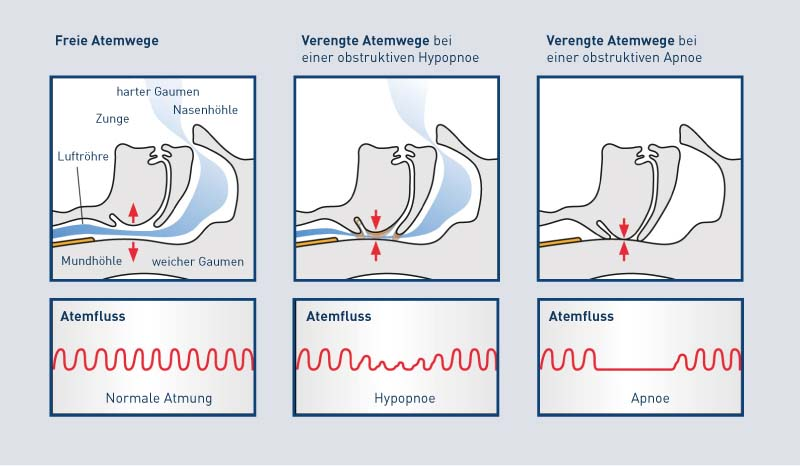
\includegraphics[width=0.55\textwidth]{introduction/was-passiert-bei-schlafapnoe}  
  \caption{Die Darstellung zeigt die Querschnittsansicht einer Person und derer Atemwege. Darunter ist der Atemfluss als Signal, welches Veränderungen während einer Atmungsstörung zeigt \cite{DeutscheFamilienversicherungSchlafapnoesyndrom}.}
  \label{introduction:problem_description}
\end{figure}

\newpage

\section{Idee}
Die Idee ist nun solche Signaleinbrüche mit maschinellem Lernen zu erkennen (siehe Abbildung \ref{introduction:problem_description}). 
Das Signal wird durch eine IMU (\textit{inertial measurement unit}) der eSense-Earpods geliefert.
Dieses Signal besteht aus 6-Achsen, den \textit{x-}, \textit{y-} und \textit{z}-Achsen des Gyroskop- und Beschleunigungssensors.
Durch eine Klassifikation, also ob in einem Zeitintervall ein Apnoeereignis vorgekommen ist, oder nicht, kann eine erste Diagnose eines respiratorischen Ereignisses bereits bequem von Zuhause aus erfolgen.
Da der Proband eine Messung mit den eSense-Earpods über viele Nächte durchführen kann, sind die Signale über einen deutlich längeren Zeitabschnitt verfügbar, als sie in einem Schlaflabor aufgezeichnet werden.

\section{Struktur}
Zu Beginn wird eine App konstruiert, welche sich mit den eSense-Earpods über BLE (\textit{Bluetooth Low Energy}) verbindet (siehe Abbildung \ref{introduction:ba_record}).
Anschließend wird eine Nutzerstudie mit 7 Personen durchgeführt, um einen Datensatz zu generieren.
Den Probanden wird über die Lautsprecher der eSense-Earpods mitgeteilt, wenn sie die Luft anhalten sollen, um eine zentrale Apnoe zu simulieren.
Anhand dieses Datensatzes kann schlussendlich ein Klassifikator trainiert werden, womit eine zukünftige Voraussage einer Messung getroffen werden kann.
Im dritten Bild der Abbildung \ref{introduction:ba_record} sind das Signal des PSG-Geräts und die Rohdaten der eSense-Earpods dargestellt. 
Zusammen bilden diese Signale neben den Kameraaufnahmen, dem Mikrofonsignal und den Nutzerinformationen einen Datensatz.
Das vierte Bild zeigt, dass nach der Klassifikation der Rohdaten, also der Gyroskop- und Beschleunigungsdaten der eSense-Earpods, eine Entscheidung darüber getroffen wird, ob in der Messung ein Apnoeereignis stattfand, oder nicht.
Die Messung wurde hierbei in viele Intervalle aufgeteilt, worauf jeweils eine individuelle Entscheidung getroffen wurde.

\begin{figure}[h]
  \centering
  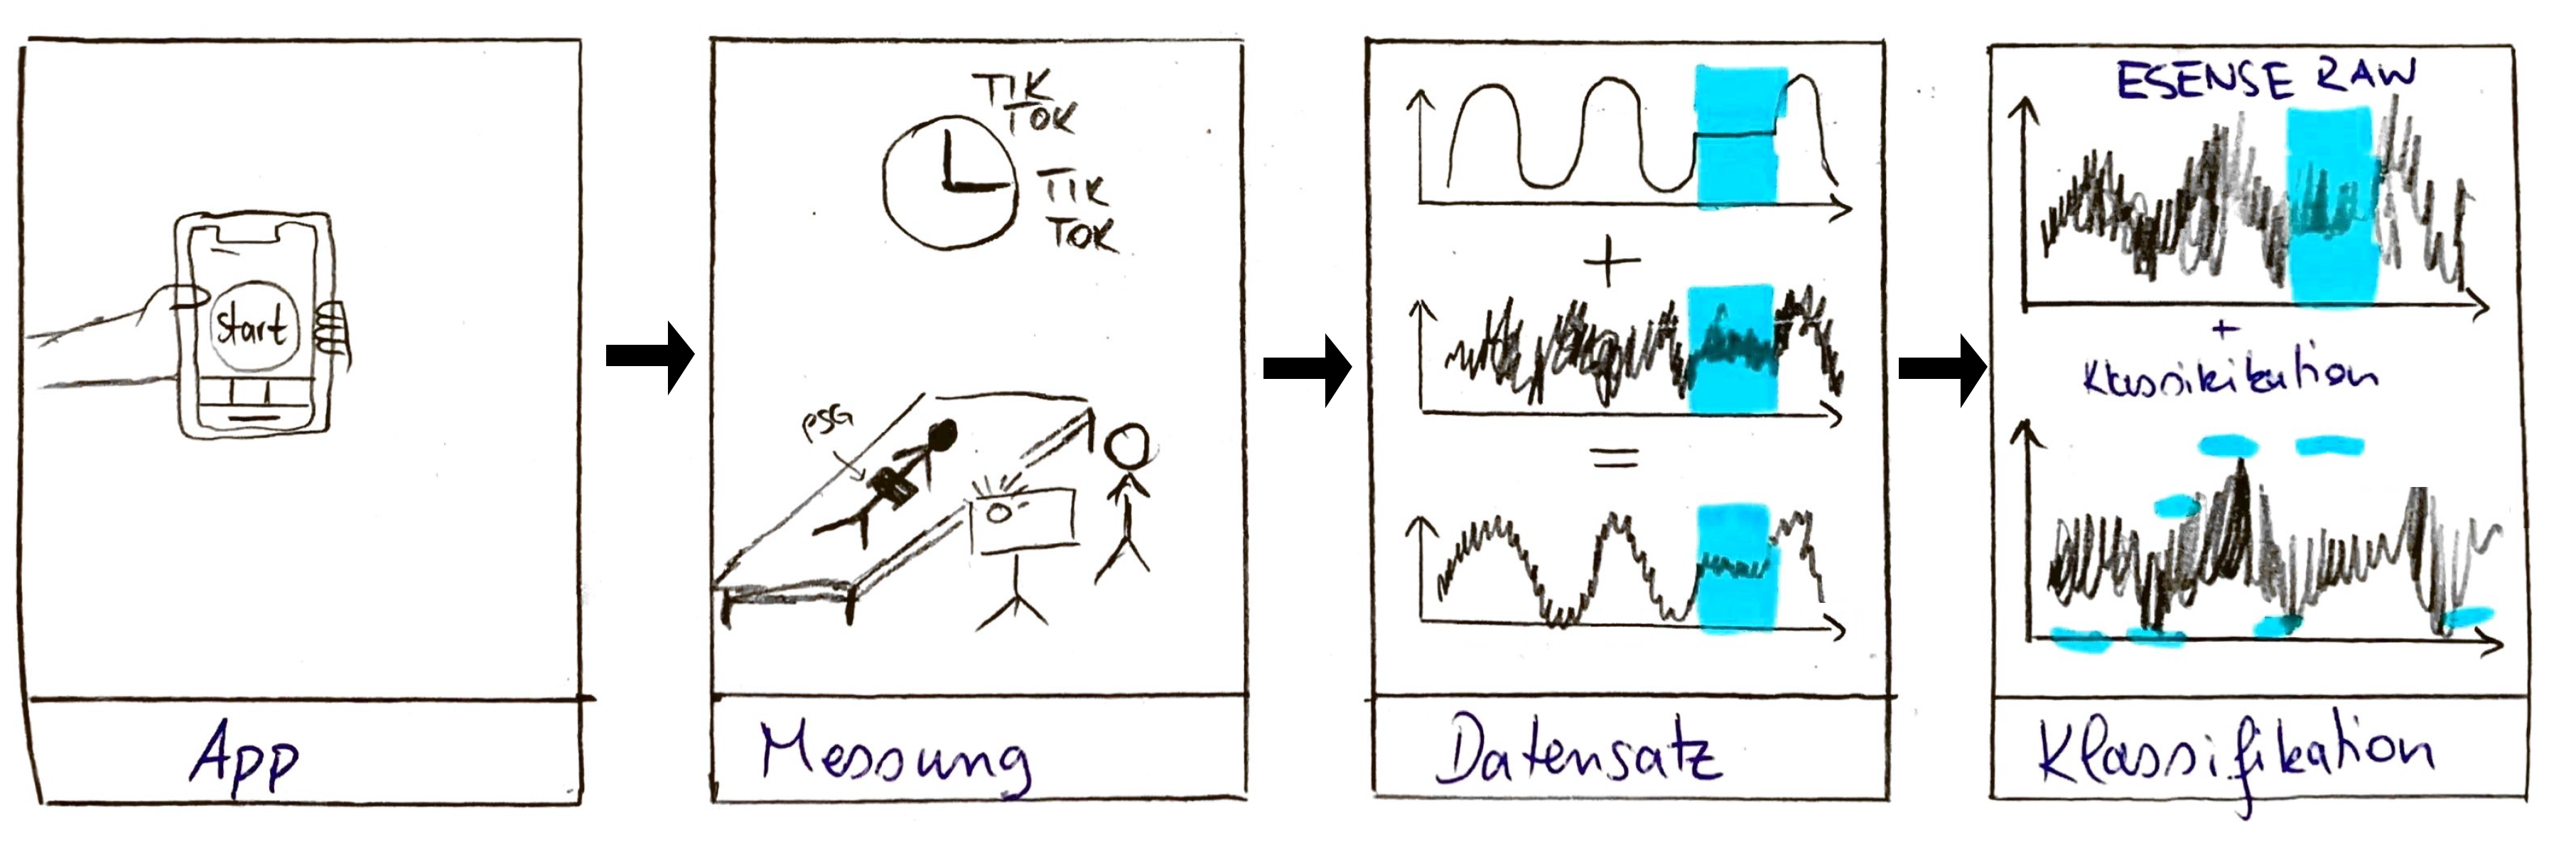
\includegraphics[width=1\textwidth]{ba_record_2}
  \caption{Darstellung des Ablaufs der Bachelorarbeit: Zu Beginn soll eine App erstellt werden, welche anschließend zur Datensammlung einer Nutzerstudie dient. Daraufhin wird ein Datensatz erstellt, welcher neben den Daten der eSense-Earpods auch den Ground-Truth beinhaltet. Anschließend wird eine Klassifikation anhand der Rohdaten der eSense-Earpods getroffen, ob ein Apnoeereignis in einem Intervall vorkommt, oder nicht.}
  \label{introduction:ba_record}
\end{figure}  % Einleitung
%% grundlagen.tex
%% $Id: grundlagen.tex 28 2007-01-18 16:31:32Z bless $
%%

\chapter{Grundlagen \& aktuelle Forschung}
\label{ch:Basics}

\section{Schlafmedizin}
\label{ch:Basics:se:schlafmedizin}
% start seite 3-5 im buch schlafmedizin_1x1 
Unter dem Begriff \textit{Schlafmedizin} versteht man die Lehre von Diagnostik, Klassifikation und Behandlung von Störungen während des Schlafs \cite{croenleinSchlafmedizin1x1Praxisorientiertes2017}. 
Trotz Er"-wäh"-nung"-en in der Antike gewinnt Schlafmedizin erst seit dem letzten Jahrhundert an Bedeutung.
Mithilfe der Polysomnographie konnten unterschiedliche Schlafphasen zyklischen Ablaufs erkannt werden.
Zudem konnten den Schlafphasen physiologische Eigenschaften nachgewiesen werden.
Heutzutage sind ca. 80 Schlafstörungen in dieversen Bereichen bekannt, welche neben psychologischen Testverfahren überwiegend elektrophysiologisch untersucht und behandelt werden.
Patienten werden mit ambulanten Hilfsmitteln oder stationär in einem Schlaflabor untersucht und diese dabei ermittelten Daten werden anschließend von technisch ausgebildetem Personal analysiert.

In einem Schlaflabor wird eine Polysomnographie durchgeführt, womit genauere Messergebnisse im Vergleich zu ambulanten Hilfsmitteln (z.B einer Langzeitbewegungsmessung) erreicht werden können.
Während einer Polysomnographie werden Gehirnströme, Augenbewegungen und Muskelspannungen erkannt, wodurch die einzelnen Schlafphasen unterschieden werden können.
Die verschiedenen Sensorwerte werden dann in Form eines Hypnogramms mittels der Kriterien des AASM (engl. \textit{American Association for Sleep Medicine}) ausgewertet (siehe Abbildung \ref{hypnogram_example}). 
Hierbei werden die Schlafstadien in \textit{Wachphase (w)}, \textit{Einschlafen (N1)}, \textit{leichten Schlaf (N2)}, \textit{Tiefschlaf (N3)} und \textit{Rapid-Eye-Movement-Schlaf (REM)} unterteilt.

\begin{figure}[ht]
    \centering
    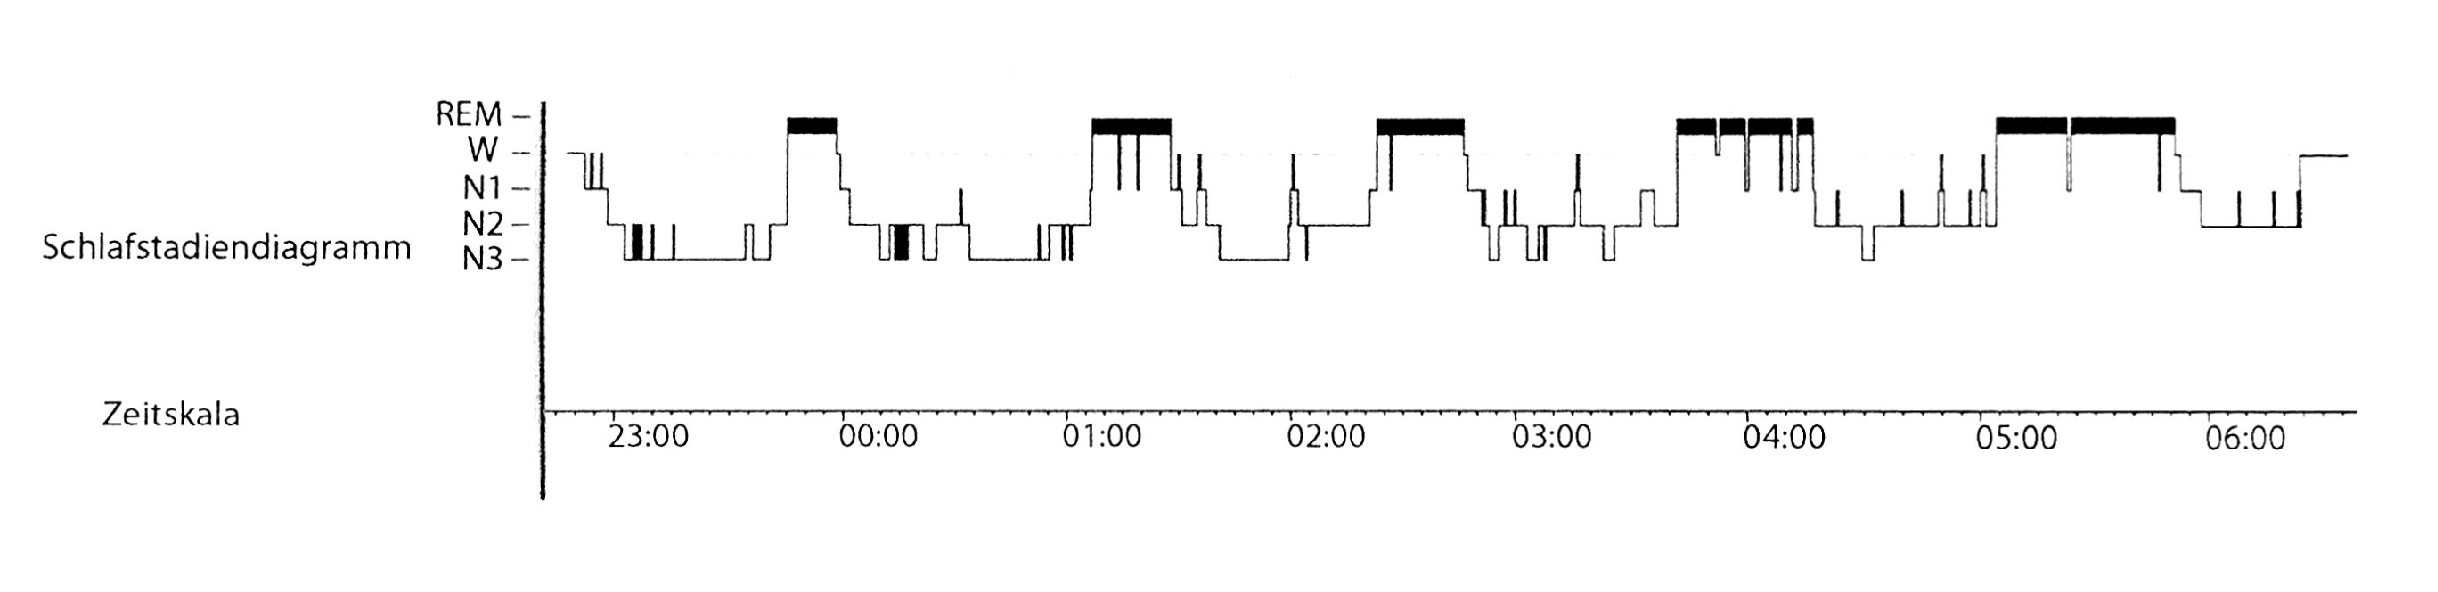
\includegraphics[scale=0.33]{respiration/hypnogram_example}
    \caption{Beispielaufzeichnung, dargestellt in einem Hypnogramm \cite{stuckPraxisSchlafmedizinDiagnostik2018}}
    \label{hypnogram_example}
\end{figure}

% ende cite
% start seite 9- im buch schlafmedizin_1x1 
Im Schlaflabor werden zudem auch Untersuchungen der Müdigkeit, der Tagesschläfrigkeit und der Aufmerksamkeit vorgenommen \cite{croenleinSchlafmedizin1x1Praxisorientiertes2017}.

Atmungsstörungen können oft die Ursache von Schlaganfällen, Herzinfarkten oder den eben genannten Symptomen sein, welche zu erheblichen psychischen Störungen führen können.
% ende cite
Aus diesem Grund ist es wichtig, so genau wie möglich Schlafstörungen bestimmen zu können, um Folgeerkrankungen zu verhindern. 

\section{Klassifizierung von Schlafstörungen}
\label{ch:Basics:se:classification}
Zur Charakterisierung von Schlafstörungen werden viele Biosignale während des Schlafs registriert, die entscheidene Merkmale liefern \cite{stuckPraxisSchlafmedizinDiagnostik2018}.
Aufgrund dieser Annahme wurde eine Einteilung in 7 Klassifikatoren für Schlafstörungen entwickelt:
\begin{itemize}
    \item Ein- und Durchschlafstörungen (Insomnien)
    \item schlafbezogene Atmungsstörungen
    \item Hypersomnien zentralnervösen Ursprungs
    \item zirkadiane Rhythmusschlafwachstörungen
    \item Störungen in Verbindung mit Schlaf, Schlafstadien oder partiellem Erwachen (Parasomnien)
    \item schlafbezogene Bewegungsstörungen
    \item andere Schlafstörungen
\end{itemize}

Diese Gliederung orientiert sich an der \textit{ICSD-3} \cite{stuckPraxisSchlafmedizinDiagnostik2018}.


Diese Bachelorarbeit ist darauf fokussiert, eine zentrale Schlafapnoe zu klassifizieren, die Bestandteil der {\glqq schlafbezogenen Atmungsstörungen\grqq} ist.
Neben der zentralen Apnoe gibt es die obstruktive Apnoe. 
Hierbei sind die Atemwege geschlossen und eine Atmung ist für mehrere Sekunden unmöglich.
Circa 20\% aller Erwachsenen haben fünf oder mehr obstruktive Ereignisse pro Schlafstunde \cite{croenleinSchlafmedizin1x1Praxisorientiertes2017}.
Zentrale Apnoe hingegen tritt seltener auf als obstruktive Apnoe, jedoch auffällig oft bei besonderen Patientengruppen. 
Ein Beispiel liefern Patienten mit Herzinsuffizienzen und einer eingeschränkten kardialen Pumpfunktion.
Unter einer zentralen Schlafapnoe leiden 72\% dieser Patientengruppe. 
Dies macht die Bedeutung der Klassifikation deutlich, da eine genaue Erkennung einer zentralen Apnoe hier sehr wichtig ist.

\subsection{Zentrale Schlafapnoe}
\label{ch:Basics:se:apnoe}
Bei der zentralen Apnoe steht der Luftfluss trotz offener Atemwege für mindestens $10\si{\s}$ still. 
Dies kann vollständig (zentrale Apnoe) oder partiell (zentrale Hypopnoe) erfolgen. 
Ab einer Anzahl von fünf Apnoeereignissen wird zentrale Apnoe diagnostiziert.
Die Ursachen gelten hierbei als internistische oder neurologische Grundlage.
Typische an- und abschwellige Muster sind auf eine chronische Herzinsuffizienz, auf eine verlängerte Kreislaufzeit oder durch eine zentralnervöse Verstellung der sogenannten Apnoeschwelle zurückzuführen.
Der $CO_2$-Gehalt im Blut wird als Apnoeschwelle bezeichnet.
Am Tag sind die Symptome der zentralen Apnoe eher an deren Ursache, den internistischen und neurologischen Grunderkrankungen, zu erkennen, da diese häufig nicht von den Symptomen der Schlafapnoe zu unterscheiden sind. 
In der Nacht wird zentrale Apnoe ebenso wie obstruktive Apnoe in Form von Atem"-aus"-set"-zern häufig vom Partner des Patienten beobachtet.
Zudem kann lautes und unregelmäßiges Schnarchen ein Indiz für eine Apnoe sein, ebenso wie ein Aufwachen in Atemnot.

Eine Schlafapnoe kann jedoch in unterschiedlichen Schweregraden auftreten. 
Es gibt Patienten, welche kaum bis keine Probleme haben und nur aufgrund von nächtlichen Erkenntnissen ihrer Partner zum Arzt geschickt werden. 
Es gibt jedoch auch Patienten, die am Tag Probleme haben, bei monotonen Situationen wach zu bleiben.

Eine Diagnose würde mögliche Folgeerkrankungen schneller erkennbar machen und die Ursache dieser erklären.

\section{Maschinelle Lernverfahren}
\label{ch:Basics:se:ml}
Zur Klassifikation einer zentralen Apnoe werden im Rahmen dieser Bachelorarbeit verschiedene Klassifikationsverfahren verwendet, welche dann zentrale Apnoeereignisse anhand der gesammelten Trainingsdaten klassifizieren sollen.

Maschinelle Lernverfahren sind Algorithmen, welche ihre Performance mittels Trainingsdaten verbessern \cite{neumannMaschineLearningKIT2020}. 
Es wird zwischen folgenden Lernverfahren unterschieden:
\begin{itemize}
    \item Supervised Learning
    \item Unsupervised Learning
    \item Reinforcement Learning
\end{itemize}
Beim \textit{Supervised Learning} sind die Trainingsdaten im Vergleich zum \textit{Unsupervised Learning} markiert.
Das heißt, dass zu jedem Eintrag ein Bit gespeichert wird, welches angibt, ob eine Apnoe zu dem Zeitpunkt stattfand, oder nicht. 
Falls ein Apnoeereignis simuliert wurde, wird eine $1$ ({\glqq positiv markiert\grqq}) eingetragen, andernfalls eine $0$ ({\glqq negativ markiert\grqq}).
Die folgenden Tabelle zeigt die verschiedenen Modelle bei \textit{Supervised} und \textit{Unsupervised Learning}:
\begin{center}
    \begin{tabular}{ | l | l | }
      \hline
      \textbf{Supervised Learning} & \textbf{Unsupervised Learning} \\ \hline
      \hline
      Regression & Clustering \\ \hline
      Klassifikation & Dimensionsreduktion \\
      \hline
    \end{tabular}
\end{center}

Jeder Algorithmus, welcher in einem dieser Modelle des maschinellen Lernverfahrens eingesetzt wird, besteht aus 3 Teilen: Zum einen der \textit{Representation}, der \textit{Evaluation} und der \textit{Optimization}. 
In der \textit{Representation} unterscheidet man nach dem zugrunde liegenden Modell, welches beispielsweise ein Entscheidungsbaum, ein neuronales Netz oder eine Support-Vektor-Maschine sein kann.
Die \textit{Evaluation} behandelt die Frage, in welche Richtung die Entscheidung getroffen werden soll. 
Beispiele hierfür wären die Genauigkeit, der Precision \& Recall, die Entropie oder der Likelihood-Schätzer.
Beim dritten Teil, der \textit{Optimization}, wird eine Optimierung des Algorithmus angestrebt. 
Dies kann unter anderem mit Methoden zweiter Ordnung, zufälliger Suche, einem absteigenden Gradienten oder der Methode der kleinsten Quadrate versucht werden.

Das in dieser Bachelorarbeit verwendete Lernverfahren ist \textit{Supervised Learning} mit dem zugehörigen Modell \textit{Klassifikation}.
Aus dem Datensatz werden Features berechnet, welche dann ein wichtiger Teil der Klassifikation sind.
Ein Feature ist ein Merkmal eines Datensatzes, welches ein individuelles, messbares Attribut der Rohdaten ist.
Pro Klassifikation werden üblicherweise eine Vielzahl an Features gesammelt, anhand derer der Klassifikator seine Entscheidungen trifft.

Zur Evaluation wurden verschiedene Klassifkationsverfahren verwendet, welche im Folgenden genauer erläutert werden.

\subsection{Random Forest}
\label{ch:Basics:se:ml:ss:randomForest}

Random Forest ist ein Klassifikationsverfahren des \textit{Supervised Learning} \cite{WaybackMachine2016}. 
Zur Klassifikation werden markierte Daten vorausgesetzt, woraus eine gelernt mathematische Repräsentation erstellt wird (\textit{model}). 
Dieses Modell wird anschließend genutzt, um auf unmarkierten Daten eine Vorhersage zu treffen.
Random Forest basiert auf Entscheidungsbäumen. 
Das sind Bäume, bei welchen pro Ast eine Entscheidung getroffen wird.
Sie lernen binäre Entscheidungsregeln, die einer logischen Abfolge entsprechen.
Jedoch sind einzelne Entscheidungsbäume nicht robust genug und neigen zu Overfitting.
Random Forest nutzt deshalb viele Entscheidungsbäume und trainiert diese auf dem selben Trainingsdatensatz. 
Der Zusammenschluss der Entscheidungen jedes Entscheidungsbaums repräsentiert die endgültige Entscheidung.
Bei Random Forest werden bei jeder Verästelung eine zufällige Teilmenge der Features in Betracht gezogen, was den Einfluss von stark korrellierenden Features verringern soll.

Entscheidungsbäume können allgemein durch verschiedene Arten zusammengetragen werden. 
Zum einen ist dies mit \textit{Bagging}, zum anderen mit \textit{Boosting} möglich.
Bei \textit{Bagging} werden zufällige Stichproben aus der Datenmenge für jeden Entscheidungsbaum genommen \cite{jamesIntroductionStatisticalLearning2013}.
Je nach Wahl geschieht dies mit oder ohne Zurücklegen dieser zufälligen Teilmenge für den nächsten Entscheidungsbaum.
Bei Bagging werden die Entscheidungsbäume parallel trainiert, was sich positiv auf die Performance auswirkt.
Bei \textit{Boosting} werden ebenfalls Teilmengen pro Entscheidungsbaum aus der Datenmenge gepickt, jedoch nicht gleichverteilt. 
Es werden schwierige Fälle höher gewichtet, wodurch diese häufiger in einen Entscheidungsbaum mit aufgenommen werden. 
Somit werden die darauffolgenden Entscheidungsbäume mit Zurücklegen der Teilmenge ausgewählt.
Falls eine falsche Vorhersage auf einen Datenbestand getroffen wurde, erhöht sich die Gewichtung.
Die Wahrscheinlichkeit ist nun höher, dass dieser Datenbestand im nächsten Entscheidungsbaum enthalten ist.
Die Entscheidungsbäume werden bei \textit{Boosting} sequenziell trainiert.

Random Forest verwendet \textit{Bagging}. 
Die endgültige Entscheidung ist entweder ein Mehrheitsvotum oder der Durchschnitt der Vorhersagen aller Trainingsläufe.
Bei Random Forest können zusätzlich einige Hyperparameter modifiziert werden, wie unter anderem die Anzahl der zu kombinierenden Entscheidungsbäume, die maximale Baumtiefe oder die maximalen Features pro Verästelung. 
Die Vorteile von Random Forest sind die Schnelligkeit, die Flexibilität und die Parallelisierbarkeit.
Zudem gibt das Resultat nicht nur die entgültige Entscheidung, sondern auch die Wahrscheinlichkeit der Entscheidung an.
Zu den Nachteilen zählt die schlechte Performance bei seltenen Klassen und die Anfälligkeit für Overfitting.
Des Weiteren ist Random Forest ein Blackbox Modell, wodurch es kaum möglich ist, zu ermitteln, wie die Entscheidung getroffen wurde.

\subsection{XGBoost}
\label{ch:Basics:se:ml:ss:xgboost}
Vor der Erklärung von XGboost muss zuvor \textit{Gradient Boosting} eingeführt werden.
Gradient Boosting ist wie Random Forest ein Teil des überwachten Lernens (\textit{Supervised Learning}) und kann für die Klassifikation oder Regression verwendet werden \cite{friedmannStochasticGradientBoosting1999}. 
Zudem ist Gradient Boosting wie Random Forest ein Ensemble-Learner, d.h. sie setzen sich aus vielen einzelnen Modellen (den Entscheidungsbäumen) zusammen.
Im Gegensatz zu Random Forest verwendet Gradient Boosting nicht \textit{Bagging}, sondern \textit{Boosting}.
Wie schon im Abschnitt \ref{ch:Basics:se:ml:ss:randomForest} eingeführt, trainiert \textit{Boosting} zufällig gewichtete Stichproben aus einer Datenmenge mit Zurücklegen. 
Falsche Entscheidungen erhöhen die Gewichtung, richtige Entscheidungen verringern die Gewichtung jeder Vorhersage. 
Somit werden schwierige Fälle besonders beachtet, da die Anpassung der Gewichtungen nach jeder Vorhersage stattfindet, insbesondere bevor die neue Teilmenge anhand der Gewichtung bestimmt wird.
Das Trainieren auf Teilmengen wird auch als stochastisches Gradient Boosting bezeichnet und verringert die Wahrscheinlichkeit für Overfitting.
Zudem wird eine bessere Generalisierbarkeit erreicht.

Zu Beginn wird ein Basismodell bestehend aus den Entscheidungsbäumen gewählt, worauf anschließend Vorhersagen anhand der Trainingsdaten getroffen werden.
Daraufhin werden die Gewichte je nach der getroffenen Vorhersage angepasst.
Aus dem Basismodell mit den nun angepassten Gewichten wird eine Teilmenge gewählt, womit erneut Entscheidungsbäume entstehen und Vorhersagen getroffen werden können.
Bei Gradient Boosting wird nun mittels Gradienten der Fehler der verschiedenen Ensembles minimiert.
Auch hier gibt es Hyperparameter, welche angepasst werden können. 
Diese sind sehr ähnlich zu Random Forest, werden jedoch um weitere Parameter ergänzt, wie zum Beispiel einer Funktion, welche den Fehler berechnet, die Anzahl der Iterationen pro Baum oder auch die Anzahl der Instanzen pro Blatt.

XGBoost ist nun eine spezielle Version des Gradient Boosting, und zwar das \textit{Extreme Gradient Boosting} \cite{chenXGBoostScalableTree2016}.
Der Unterschied zu Gradient Boosting ist hierbei, dass bei der Fehlerfunktion (Loss-Funktion) die Gradienten 2. Ordnung gewählt werden, wodurch mehr Informationen für die Verringerung des Fehlers bereit stehen.
Zudem können dadurch die besten Entscheidungsbäume approximiert werden. 
XGBoost verwendet außerdem L1 \& L2 Regularisierung, dadurch kann besser generalisiert werden und Overfitting vermieden werden.
XGBoost ist parallelisierbar, schnell und kann zudem für verteiltes Trainieren auf Clustern betrieben werden.

\subsection{Support Vektor Maschine (SVM)}
\label{ch:Basics:se:ml:ss:svm}
Eine Support Vektor Maschine ist ein Klassifikationsverfahren für Probleme, welche in zwei Klassen gruppiert werden \cite{cortesSupportvectorNetworks1995}.
Bei der linearen Support Vektor Maschine wird nun eine lineare {\glqq Trennlinie\grqq} gesucht, welche die Menge der Daten in zwei Klassen gruppiert. 
Diese Trennlinie wird optimiert.
Es gibt auch eine nichtlineare SVM, die eine nichtlineare Trennlinie sucht.
Hierbei kann es jedoch zu Overfitting kommen, da eine nichtlineare Trennlinie durch potenzielle Outlier sehr komplex werden kann und zu {\glqq gut\grqq} optimiert wird.
Jeder Wert im Datensatz ist ein Support Vektor und somit ein repräsentativer Punkt, welcher bei der Klassifikation gruppiert werden soll.
Die Trennlinie muss also zwischen allen markierten Daten unterscheiden können.
Jedoch ist die Komplexität hierbei sehr hoch, da eine Trennlinie beziehungsweise eine Trennebene im hochdimensionalen Raum, nur mit sehr hohem Aufwand gefunden werden kann.
Die Suche nach der Trennline kann mit unterschiedlichen Kernel bestimmt werden.
Die beliebtesten Kerneltypen sind:

\begin{center}
    \begin{tabular}{ | l | l | }
        \hline
        Kernel Name & Kernel Funktion \\ \hline
        Linear Kernel & $K(x)=x \cdot y$ \\ 
        Polynomial Kernel & $K(x)=(x\cdot y+1)^d$ \\
        Radial Basis Function (RBF) Kernel & $K(x)=e^{-\gamma(\Vert x-y \Vert)^2}$ \\
        \hline
    \end{tabular}
\end{center}

Die korrekte Wahl des richtigen Kernels ist entscheidend für deren Performance und Genauigkeit, jedoch nicht sehr einfach.
Ein Vorteil von SVM ist die Effektivität im hochdimensionalen Raum.
Des Weiteren ist SVM speichereffizient und zudem können durch die verschiedenen Kerneltypen mehrere Datensätze variabler verarbeitet werden.
Zu den Nachteilen zählt, dass die Performance schlecht ist, wenn die Anzahl der Features größer als die Anzahl der Samples ist. 
Zudem neigt SVM gerade im nichtlinearen Bereich schnell zu Overfitting.

\section{Forschung von Klassifikation anhand von IMU-Daten}
Es gibt bereits Ansätze, welche sich damit befassen, Alternativen zur Ermittlung von Schlafstörungen zu finden. 
Somit könnte ein Besuch im Schlaflabor durch einen bequemen Test ersetzt werden. 
Ein vielversprechender Ansatz ist es, mittels IMU-Daten die Bewegung des Körpers zu messen und anhand dieser Informationen unter anderem die Atmung herauszufiltern, um dann Rückschlüsse auf Schlafstörungen ziehen zu können.

\subsection{Beschleunigungssensor am Brustkorb}
Bereits 2018 gab es Forschung in diesem Bereich. \textit{Phan Duy Hung} hat sich damit befasst, einen Beschleunigungssensor (\textit{Accelerometer}) an den Brustkorb zu fixieren \cite{hungCentralSleepApnea2018}.
Durch die Platzierung an genau dieser Stelle wurde der Herzschlag genauer erkannt. 
Die Rohdaten zeigen hierbei bereits die Herzfrequenz und die Atmung des Probanden (siehe Abb. \ref{imu_research_hung_rawData}). 

\begin{figure}[ht]
    \centering
    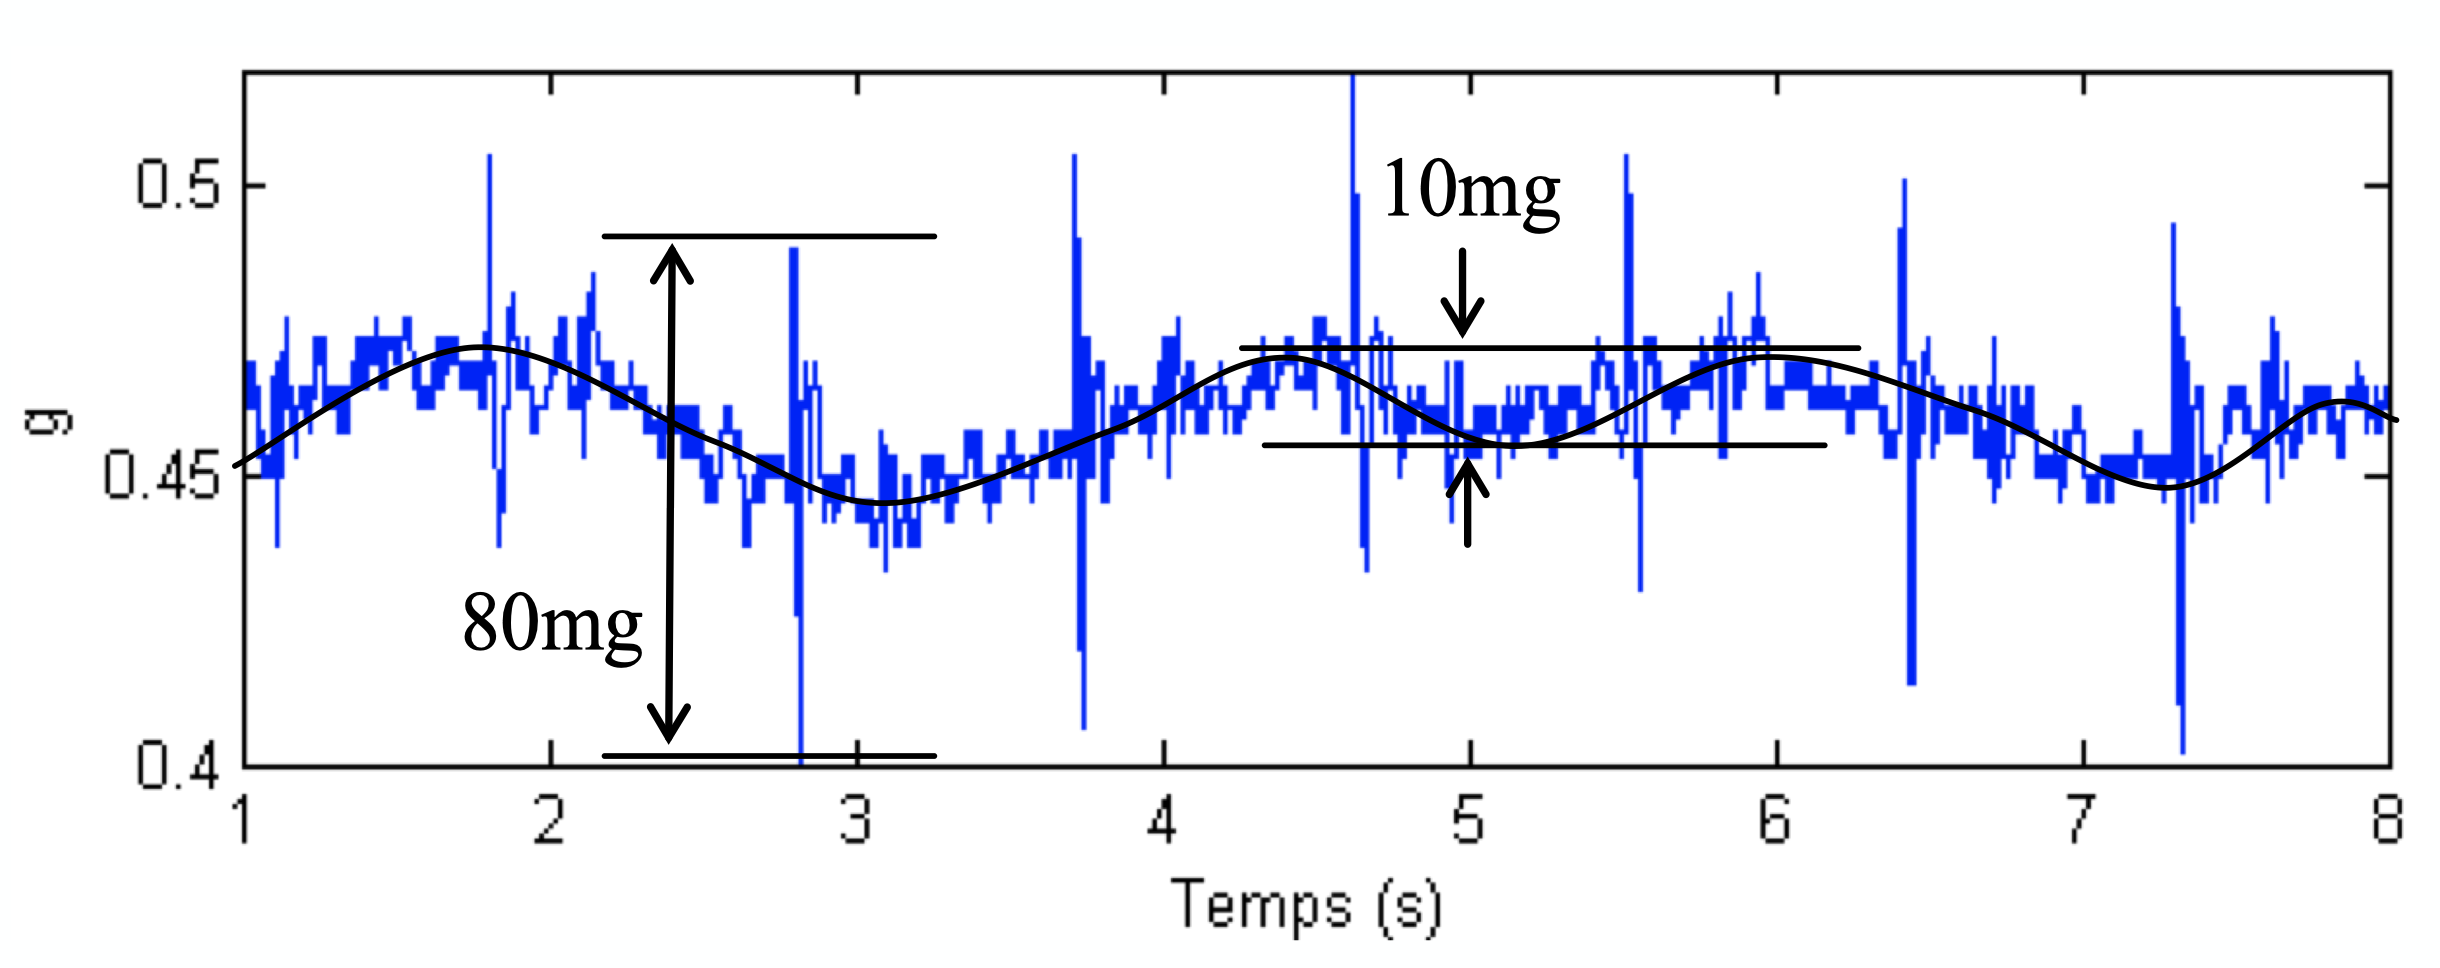
\includegraphics[width=1\textwidth]{imu_research/Paper_Hung_rawData}
    \caption{Rohdaten des Accelerometers in \cite{hungCentralSleepApnea2018}}
    \label{imu_research_hung_rawData}
\end{figure}

Die Daten wurden nach der Aufzeichnung durch einen Bandpassfilter mit adaptiver Apassung optimiert, um die SNR (\textit{signal-noise-ratio}) zu verringern.
Der Puls wurde ermittelt, indem Peaks (Max: \textit{V}-Peak, Min: \textit{R}-Peak) gefunden und als Herzschlag interpretiert wurden.
Des Weiteren musste Signalrauschen, beispielsweise von der Reibung des T-Shirts und der Haut, aus dem Signal herausgefiltert werden. 
Zudem wurden 3 Features anhand der Amplitude über die Zeit berechnet. 
Das erste Feature ist das \textit{Spektralverhältnis (spectral ratio)}. 
Hier wird ein Leistungsspektrum eines einminütigen Segments vom HR-Signal geschätzt. 
Der Frequenzbereich zwischen $[0,1]\si{\hertz}$ wurde untersucht. 
Dieser Bereich spiegelt die Frequenzvariation zwischen zentraler Schlafapnoe und normaler Aktivität wieder.

Im Bereich von $[0.3,0.6]\si{\hertz}$ zeigt sich das Maximum der spektralen Leistung.
Dieser Wert wird normiert, indem er durch den Mittelwert der spektralen Leistung im Bereich $[0.1,0.3]\si{\hertz}$ geteilt wird. 
Das Verhältnis von $\max(P)$ im Bereich von $[0.3,0.6]\si{\hertz}$ zum Mittelwert($P$) in $[0.1,0.3]\si{\hertz}$ ist unabhängig von der Person $P$.

Das zweite Feature sind die \textit{Wavelet- Koeffizienten (wavelet coefficients)}, bei welchen für die Analyse mit mehreren Auflösungen und guter Lokalisierungsfähigkeit im Zeit-Frequenz-Bereich häufig eine Wavelet-Transformation verwendet wird. 
Hierbei wird das Atemsignal in 5 Ebenen mit der db2-Wavelet zerlegt. Danach werden die Standardabweichungen der Detailkoeffizienten in den Ebenen 4 und 5 verwendet. 

Das dritte Feature sind die \textit{linear prediction coefficients}. 
Die lineare Vorhersage zweiter Ordnung
\begin{center}
    $x(n) = a_1 x(n-1) + a_2 x(n-2) + e(n)$
\end{center} 
wird verwendet, wobei $x$ eine Zeitreihe (\textit{Timeseries}) ist, $e(n)$ der Vorhersagefehler und {a1, a2} die Vorhersagekoeffizienten, die durch die Kleinste-Quadrate-Methode zu bestimmen sind.

Nach einer Varianzanalyse (\textit{ANOVA}) werden die folgenden Werte ausgewählt: \\
ANOVA: $a_1$, $a_2$ und $\sqrt{a_1^{2} + a_2^{2}}$.


Zudem wurden nichtlineare Features in Betracht gezogen, da bereits vorher festgestellt wurde, dass in komplexen Atemuntersuchungen lineare Funktionen nicht ausreichen. Die Herzfrequenz wurde hierbei als Zeitreihe (\textit{Timeseries}) betrachtet.
Es wurden diesbezüglich die nichtfunktionalen Features der \textit{Poincaré-Plots (Poincare plot geometry)}, \textit{trendbereinigende Fluktuationsanalyse (Detrended Fluctuation Analysis)}, \textit{ungefähre Entropie (Approximate Entropy)} sowie der \textit{Ljapunow-Exponent (Largest Lyapunov exponent)} verarbeitet. 

Die Features wurden anschließend mit der \textit{ANOVA-Toolbox} ausgewertet.
Somit konnte ermittelt werden, ob in dem zeitlichen Intervall eine Apnoe stattgefunden hat, oder nicht.

Durch dieses Paper wurde eine Genauigkeit von 84.2\% erreicht, eine zentrale Apnoe als solche zu erkennen.
Zudem wurde zu 84.1\% erkannt, dass in diesem Zeitrahmen keine zentrale Apnoe vorkam.


\subsection{Detektion direkt am Kopf mittels der Google-Glass Brille}
Bereits 2015 wurde versucht, durch Informationen des Google-Glass den Puls und das Atemsignal zu ermitteln \cite{hernandezCardiacRespiratoryParameter}. 
Der Vorteil hierbei ist die Position der Brille. 
Da sie am Kopf platziert ist, liefert die Brille andere Werte im Vergleich zu IMU-Daten, die am Brustkorb aufgezeichnet werden.
In Abbildung \ref{imu_research_google_glass} ist die Google-Glass Brille zu sehen.
Der Gyroskop- und Beschleunigungssensor ist an der rechten Seite angebracht, ebenso wie eine Kamera, ein Magnetometer, ein Lightsensor und ein Mikrofon. 
Obwohl die Google-Glass Brille nicht entwickelt wurde, um physiologische Daten zu sammeln, kann sie dafür verwendet werden, da alle nötigen Sensoren darin verbaut sind.
Die Resultate liefern einen mittleren absoluten Fehler (\textit{MAE}) von 0.82 Schlägen pro Minute (STD: 1.98) der Herzrate und 0.6 Atmungen pro Minute (STD: 1.19) bei der Atmung unter Betrachtung verschiedener Beobachtungsfenster und Kombinationen der Sensoren. 

\begin{figure}[ht]
    \centering
    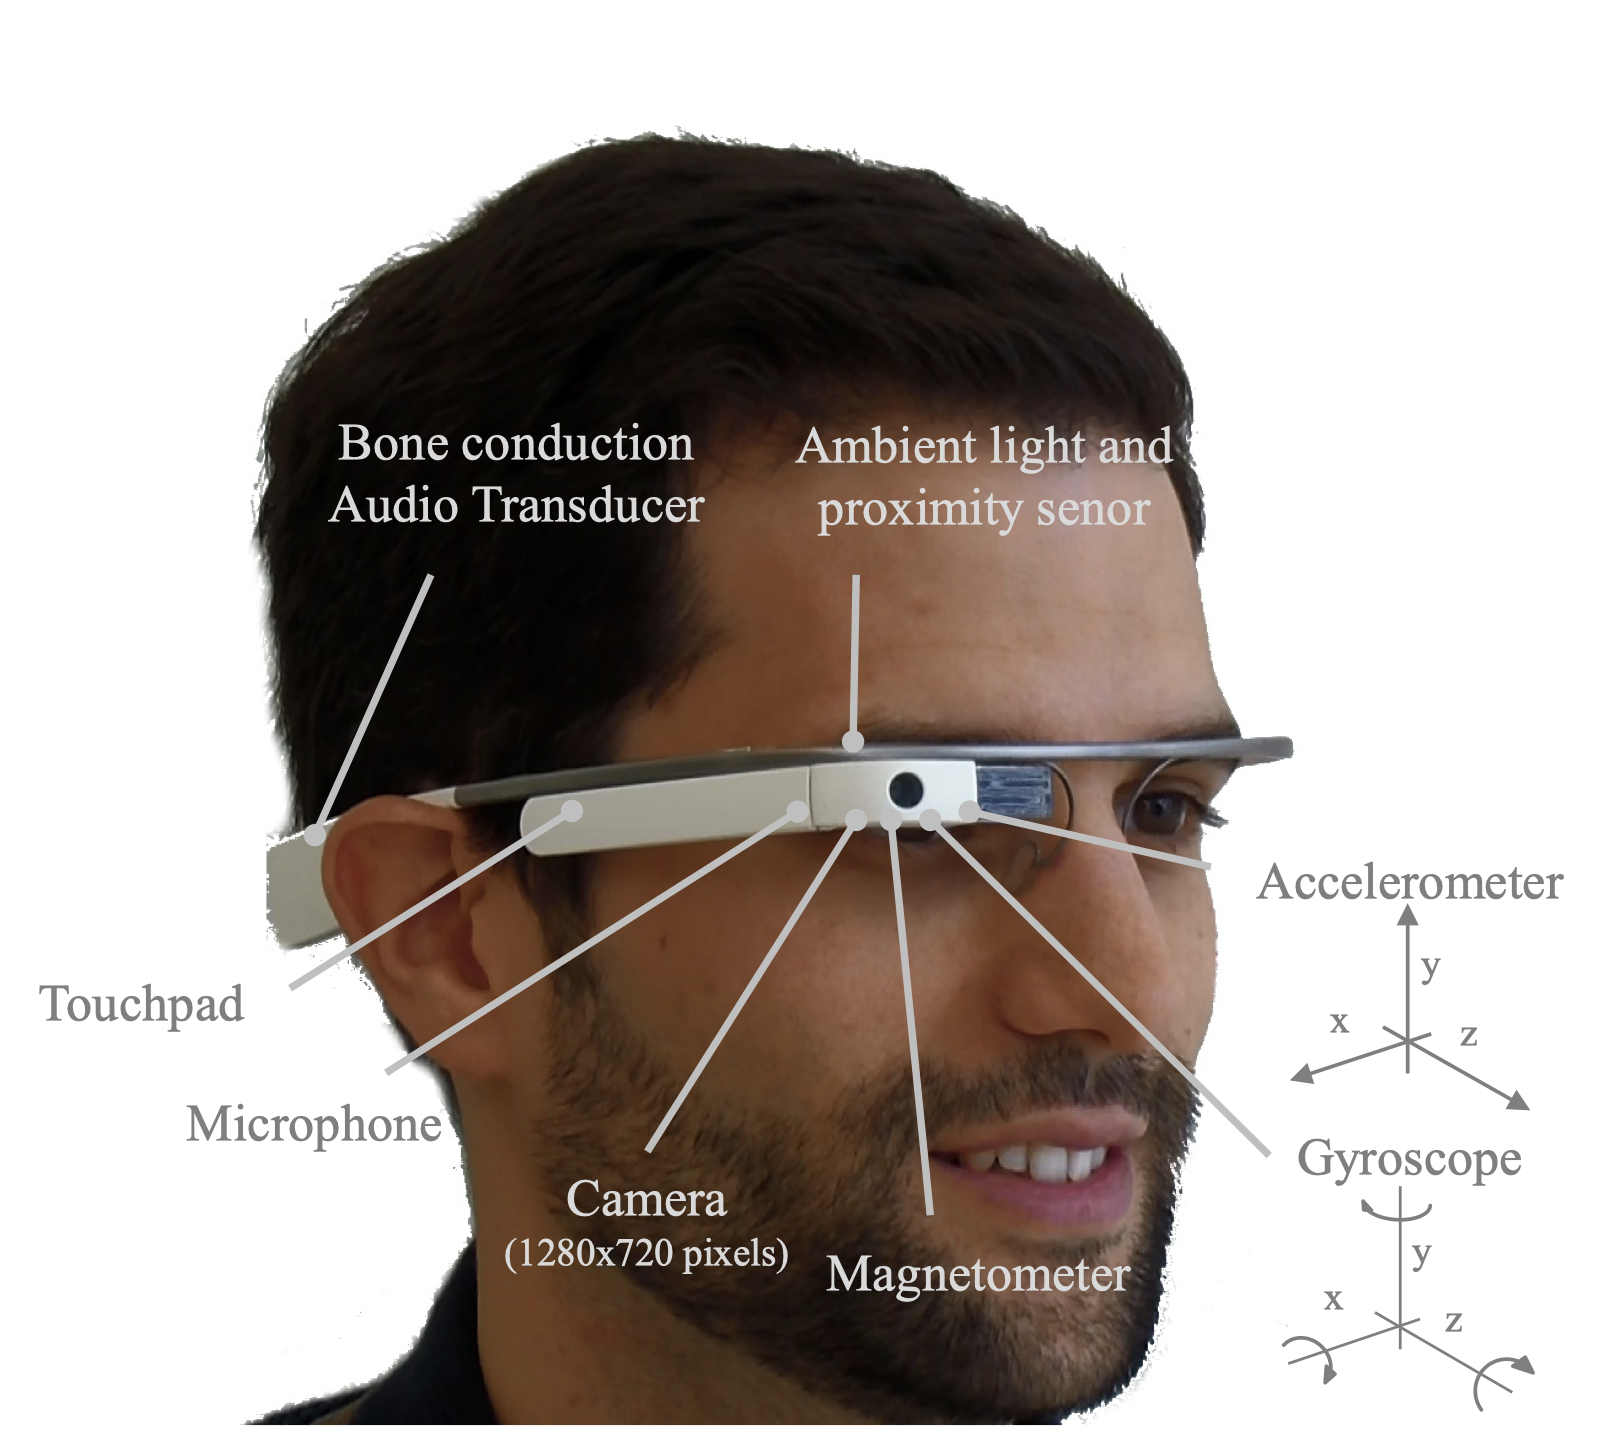
\includegraphics[width=\textwidth / 2]{imu_research/googleGlass}
    \caption{Darstellung der Google-Glass Brille: Die Brille hat einen Magnetometer, einen Gyroskop- und Beschleunigungssensor, eine Kamera, ein Mikofon und einen Lichtsensor verbaut. Diese Sensoren werden genutzt, um die Atmung und den Puls zu ermitteln. \cite{hernandezCardiacRespiratoryParameter}}
    \label{imu_research_google_glass}
\end{figure}
Die Herausforderung bestand zudem darin, stromsparende Echtzeitberechnungen mit Algorithmen zu entwickeln, womit physiologische Parameter extrahiert wurden. Der Nutzer soll das Gerät im Alltag normal weiternutzen können. 

Es wurden 2 Techniken entwickelt, eine zur Ermittlung des Pulssignals, die andere für das Atemsignal.
\subsubsection{Pulssignal}
Die Schätzung des Pulssignals wurde anhand einer Zeitreihe (\textit{Timeseries}) von Vektoren in mehrere Schritte aufgeteilt:
\begin{itemize}
    \item Von jeder Dimension des Vektors wurde ein gleitendes Durchschnittsfenster von 3 Abtastwerten subtrahiert, wodurch Signalverschiebungen und Trends entfernt werden konnten.
    \item Ein Bandpass Butterworthfilter der 4. Ordnung mit den Cut-Off Frequenzen von $10 \si{\hertz}$ und $13 \si{\hertz}$ wurde auf jede Dimension angewandt, um Veränderungen des BCG (\textit{Ballistokardiogramm}) zu isolieren.
    \item Zudem wurde ein Bandpass Butterworthfilter der 2. Ordnung mit den Cut-Off Frequenzen von $0.75 \si{\hertz}$ und $2.5 \si{\hertz}$ (entspricht 45 and 150 Schlägen pro Minute) angewandt, was schließlich das resultierende Pulssignal liefert.
\end{itemize}

\begin{figure}[ht]
    \centering
    \begin{subfigure}{.49\textwidth}
        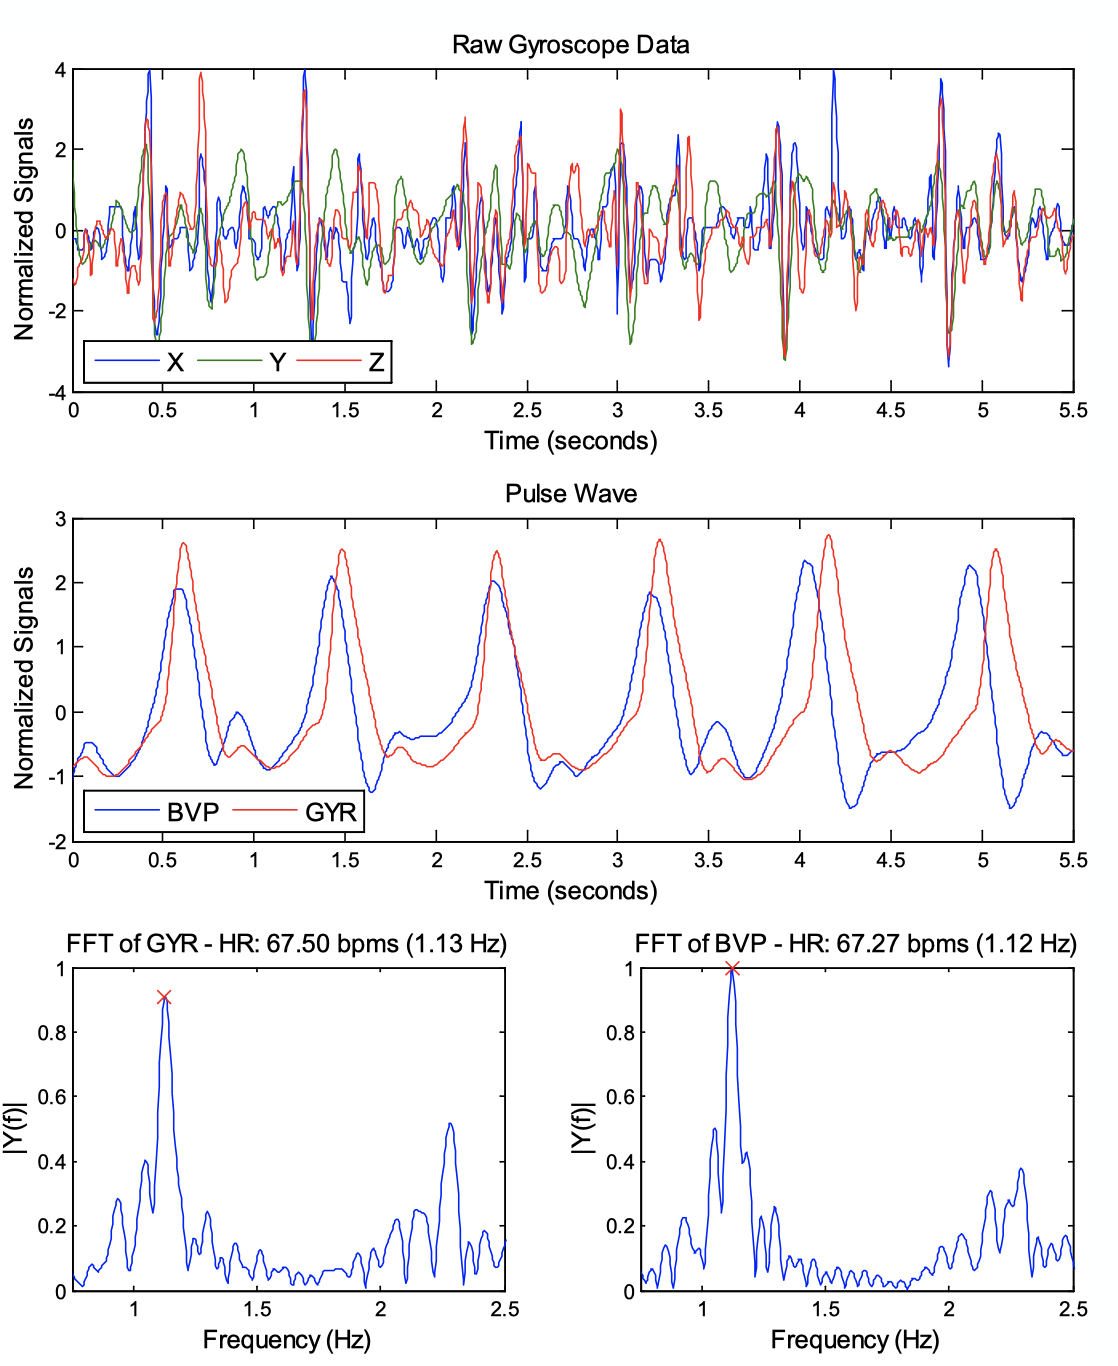
\includegraphics[width=\textwidth]{imu_research/googleGlass_pulse_fig2}
      \caption{Beispiel eines Pulssignals mittels der Gyroskopdaten (rot) und des Ground-Truth Sig"-nals (blau). Die beiden unteren Graphen zeigen das Fouriespektrum von jedem Signal (\textit{FFT: Fourier Spectrum, GYR: Gyroscope, BVP: Blood Volume Pulse, HR: Heart Rate, bpms: beats per minute})}
      \label{background:googleGlass:pulse_wave}
    \end{subfigure}
    \begin{subfigure}{.49\textwidth}
        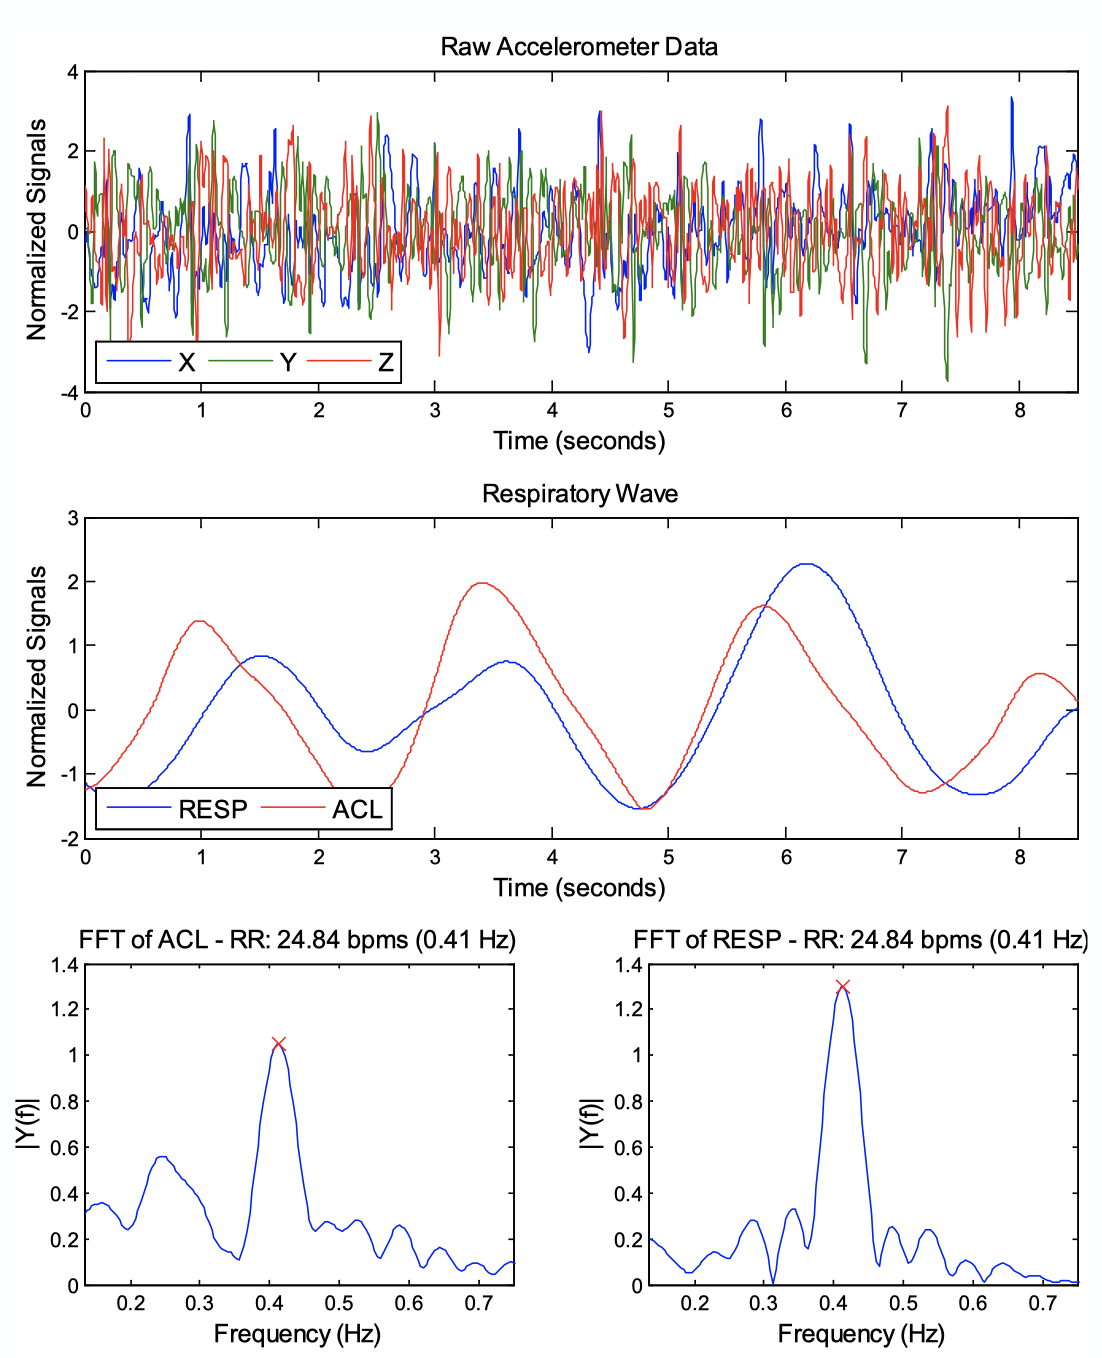
\includegraphics[width=\textwidth]{imu_research/googleGlass_respiratory_fig3}
      \caption{Beispiel einer Schätzung des Atemsignals anhand der Beschleunigungsdaten (blau) und des Ground-Truth-Signals (rot). Die beiden unteren Graphen zeigen das Fourierspektrum jedes Signals. (\textit{FFT: Fourier Spectrum, ACL: accelerometer, RESP: Respiration from chest band, RR: respiration rate, bpms: breaths per minute})}
      \label{background:googleGlass:respiratory_wave}
    \end{subfigure}
    \caption{Herzrate- und Atemfrequenzanalyse}
    \label{background:googleGlass}
  \end{figure}

Die Abbildung \ref{background:googleGlass:pulse_wave} zeigt ein Signal des Herzschlags, gesammelt von den Informationen der Gyroskopdaten. Diese Daten wurden mit der Google-Glass Brille aufgezeichnet, während die Person auf dem Rücken lag. Der obige Graph zeigt ein 3-Achsen Gyroskopsignal über eine Dauer von 5.5 Sekunden. Der mittlere Graph zeigt die Schätzung des Herzschlags, nachdem die vorgestellten Methoden angewandt wurden in rot, die des Referenzsignals in blau. Es ist sehr gut zu erkennen, dass die Schätzung sehr nahe an den Referenzsignalen ist.

\subsubsection{Atemsignal}
Das Atemsignal wurde in mehreren Schritten berechnet:
\begin{itemize}
    \item Ein gleitender Mittelwertfilter wurde auf jede Komponente angewandt. Die Fensterlänge wurde auf die Dauer eines Atemzyklus gesetzt, in diesem Fall 45 Atmungen pro Minute. 
    \item Ein Bandpass Butterworthfilter der 4. Ordnung mit den Cut-Off Frequenzen von $0.13 \si{\hertz}$ und $0.75 \si{\hertz}$ (entspricht 8-45 Atmungen pro Minute) wurde auf jede Dimension angewandt.
    \item Da die verschiedenen Dimensionen der Sensoren nicht in Relation zu den Körperpositionen stehen, wurde eine Principal Component Analyse angewandt, um einen derartigen Einfluss zu reduzieren. Nach einer Fast Fouriertransformation (FFT) auf jede Komponente wurde das Signal mit der Periode mit der maximalen Größe ausgewählt, welche innerhalb des zu betrachtenden Frequenzbereichs liegt.
\end{itemize}

Die Abbildung \ref{background:googleGlass:respiratory_wave} zeigt ein Beispiel einer Atemfrequenzschätzung der Beschleunigungsdaten eines Patienten. Wie zu sehen ist, sind die Daten sehr nahe an dem Referenzwert, welcher als Ground-Truth mit dem Brustgurt mit aufgezeichnet wurde.


\subsection{Überwachung von Puls und Atmung mittels eSense-Earpods}
Im Jahr 2019 wurde von \textit{Tobias Röddiger}, \textit{Daniel Wolffram} und \textit{David Laubenstein} nachgewiesen, dass es möglich ist, mittels den eSense-Earpods die Atmung und den Puls annähernd zu ermitteln \cite{roddigerRespirationRateMonitoring2019}. 
Dies gelang etwas genauer als das Monitoring von \textit{J. Hernandez} mit dem Google Glass \cite{hernandezCardiacRespiratoryParameter}.
Es wurde hierbei eine Studie mit 12 Personen aufgezeichnet, welche in 3 Positionen (liegend, stehend, sitzend) jeweils vor beziehungsweise nach einer sportlichen Bewegungsphase einen einminütigen Atemablauf durchgeführt haben. 
Die Analyse der Daten erfolgte im Anschluss der Studie.
Dabei wurden die Daten in einer Pipeline verarbeitet, welche zuerst das Rauschen reduzierte, anschließend einen Triangle-Filter der Breite $2\si{\s}$ anwendete und danach eine PCA (engl. \textit{principal component analysis}) ausführte, um die Daten unabhängig von deren Achse zu bewerten.
Nun wurden Fenster mit der Größe von $20\si{\s}$ extrahiert, anhand welchen Atmung und Puls berechnet wurde.
Die Resultate ergaben einen mittleren absoluten Fehler (engl. \textit{mean absolute error}) von 2.62 CPM (acc) und 2.55 CPM (gyro), jedoch variierten diese von Proband zu Proband.

Der Ablauf der Analyse begann damit, dass ein gleitendes Durchschnittsfenster (\textit{sliding average window}) von 3 Samples von jeder Dimension abgezogen wurde. 
Zudem wurde auf jeder der Komponenten ein Mittelwertfilter angewandt. 
Diese haben eine Fenstergröße von 2 Sekunden. 
Das soll Signalverschiebungen und Signaltrends entfernen.
Anschließend wurde eine kubische Splineinterpolation auf den Datensatz angewandt, um die Daten aufzublasen.
Falls zuviel Bewegung in einem Fenster zu erkennen ist, wurde das Fenster verworfen \cite{sunSleepMonitorMonitoringRespiratory2017}.
Daraufhin wurde ein Bandpass-Butterworth-Filter der 4. Ordnung auf den Datensatz angewandt, um das Rauschen zu entfernen.
Zum weiteren Glätten der Signale wurde ein Dreiecksfilter angewandt \cite{haotianMindfulWatch2017}, worauf schließlich eine Hauptkomponentenanalyse (PCA) durchgeführt wurde.
Auf jede Hauptkomponente wurde nun eine Spektralanalyse mithilfe einer Fourier-Transformation (FFT) angewandt. 
Die Frequenz, welche dem Peak mit der höchsten Magnitude entspricht, resultiert schlussendlich als Atemfrequenz.

\begin{figure}[ht]
    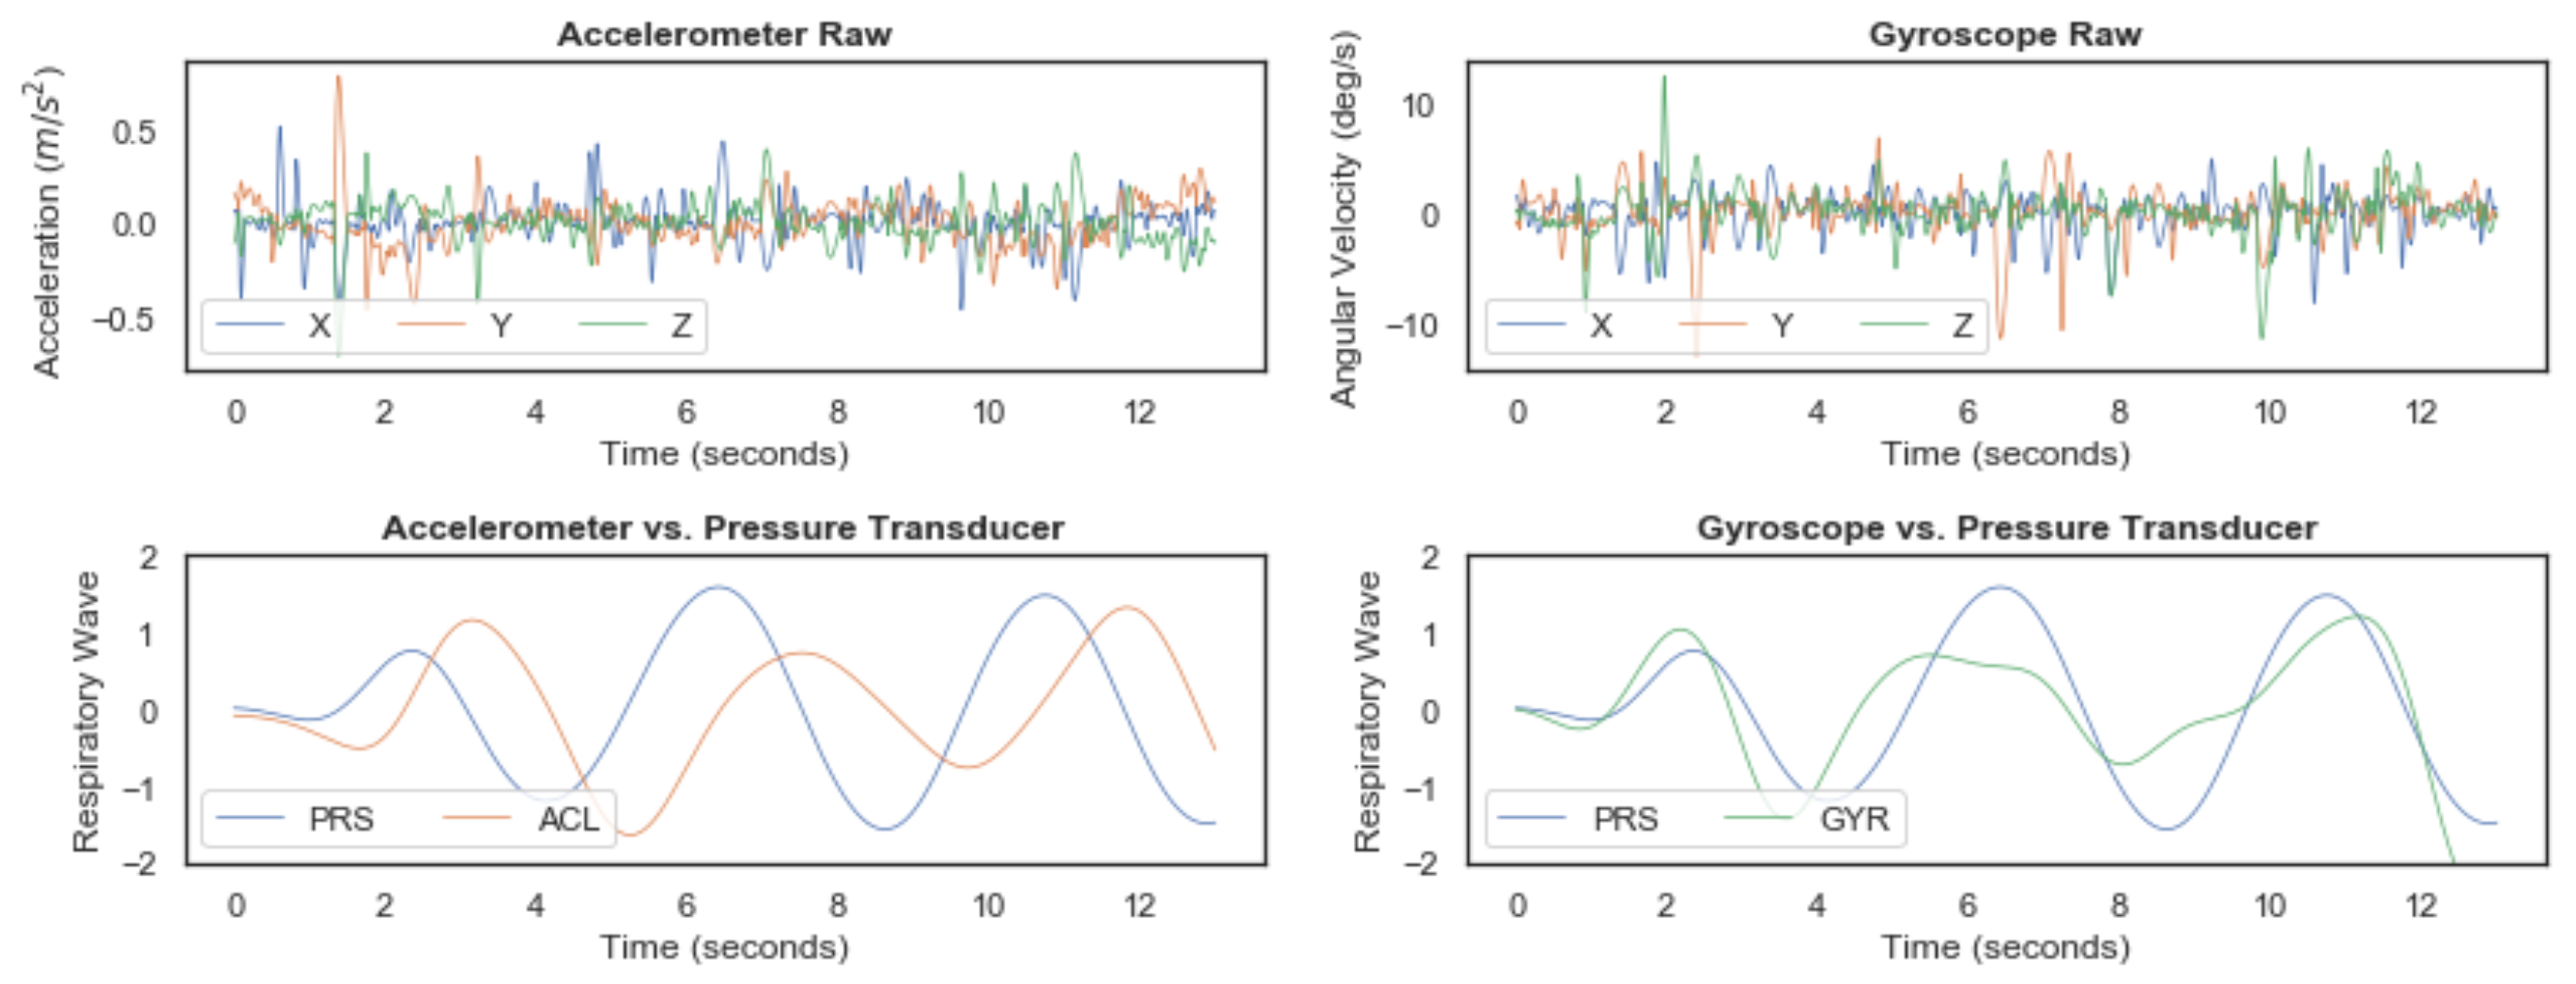
\includegraphics[width=1\textwidth]{imu_research/towards_resp_rates_waves}
    \caption{Rohdaten der Beschleunigungs- und Gyroskopdaten innerhalb von $12 \si{\s}$, sowie die Atem- und Pulsschätzung, verglichen mit dem Ground-Truth (blau).}
    \label{background:towards_resp_esense:results}
\end{figure}  % Grundlagen
%% analyse.tex
%% $Id: analyse.tex 28 2007-01-18 16:31:32Z bless $

\chapter{Schlafanalyse}
\label{ch:sa}

\section{Earable Plattform}
\label{ch:sa:ep}
Zur Erfassung der Daten werden eSense-Earpods der Firma ``Nokia Bell Labs Cambridge'' verwendet.	
Es ist ein Mikrofon und Lautsprecher verbaut, welche beide über Bluetooth angebunden werden können. 
Des weiteren ist das für diese Bachelorarbeit interessanteste Element, eine 6-Achsen IMU (Inertial Motion Unit) enthalten.
Eine IMU ist eine inertiale Messeinheit, womit Gyroskop- und Beschleunigungsdaten aufgezeichnet und mittels BLE (Bluetooth Low Energy) auf das Smartphone übertragen werden können. 
Es handelt sich um einen 3-Achsen Beschleunigungssensor, sowie einen 3-Achsen Gyroskop.
Die Messrate dieser Sensoren ist variabel einstellbar, wurde im folgenden auf $50 \si{\hertz}$ festgelegt.

\todo{Beschreibe noch die Filter, die auf die Daten angewandt werden per Default... steht in der Doku des eSense Kopfhörers}

\todo{import picture of esense earpods}

\todo{soll ich hier schreiben, dass die Kopfhörer noch nicht im Handel sind?}

\todo{Welche Vor-/Nachteile gibt es diese zu nutzen? Was soll auf genommen werden?}

\subsection{Was wird aufgezeichnet?}
\label{ch:sa:ep:what_to_record}
Zu vollständigen Aufzeichnung eines Datensatzes werden die IMU-Daten, welche via BLE auf das Smartphone übertragen werden, in einer Datenbank abgespeichert.
Insgesamt werden hierbei pro empfangene Dateneinheit 6 Werte persistiert, die \textit{x, y} und \textit{z} Richtung vom Beschleunigungssensor, bzw vom Gyroskop. 
Des weiteren wird die aktuelle Zeit, die aktuell auszuführende Aktion des Studienablaufs und die Information, ob die LED des Smartphones an oder aus ist, zu jeder empfangenen Dateneinheit hinzugefügt.
Das Mikrofon wird ebenfalls aufgezeichnet und nach der Messsung abgespeichert.
Vor dem Beginn einer Messung wird der Studienteilnehmer gebeten, ein paar Zusatzinformationen (siehe \ref{ch:sa:additionalUserStudiesInformation}) anzugeben.
Diese werden vor dem Start der Messung am Smartphone ausgefüllt und ebenfalls in der Datenbank gespeichert.

\subsection{Datenexport}
\label{ch:sa:ep:export}
Zur weiteren Verarbeitung werden die Daten, nachdem sie von der App lokal in einer Datenbank gespeichert werden, exportiert. 
Zuerst werden die Datenbankeinträge der aktuellen Messung als \textit{csv}-Datei exportiert und in einem temporären Ordner abgespeichert.
Hierbei werden die Gyroskop einträge separat von den Beschleunigungsdaten exportiert, es entstehen folglich 2 \textit{csv}-Dateien (\glqq \textit{GyroData\_\$ID\$.csv}\grqq, \glqq \textit{ACCData\_\$ID\$.csv}\grqq).
Das Mikrofon-Signal wird nach der Messung als \textit{m4a}-Datei ebenfalls im temporären Ordner abgelegt.
Die Zusatzinformationen, welche über den Studienteilnehmer hinterlegt wurden, werden als \textit{csv}-Datei (\glqq \textit{UserStudyPersonDetails\_\$ID\$.csv}\grqq) ebenfalls in den temporären Ordner persistiert.
Alle Dateien des temporären Ordners werden in einer zip-Datei verpackt und können über den Share-Screen von Apple über verschiedene Wege geteilt werden.

\section{Polysomnographie-Systeme}
\label{ch:sa:psg}
Als Referenz zu den eSense-Earpods wird ein Polysomnographie-System (PSG-System) verwendet. 
Ein solches System zeichnet Messungen für physiologische Funktionen des Körpers währrend des Schlafs auf und kann somit mögliche Schlafstörungen diagnostizieren.
Es werden kontinuierlich verschiedene Körperfunktionen überwacht, wodurch nach einer Messung ein umfangreiches und individuelles Schlafprofil erstellt werden kann.

Das Polysomnographie-System zeichnet währrend der Studie ebenfalls Daten auf und soll die Resultate, welche durch die eSense-Earpods gesammelt und analysiert werden, verifizieren. Somit dienen die Daten, welche durch das PSG-System gesammelt werden, als \glqq Ground-Truth\grqq.

\todo{erkläre, wie man das PSG-System konfigurieren kann, dass es ein programm gibt, wo man eine Montage definieren kann, was ich gewählt habe, warum}

Im folgenden werden alle Sensoren aufgelistet, welche für die Studie aufgezeichnet wurden. Die nicht persistierten Daten werden im folgenden ignoriert.

\todo{übersetze tabelle und erkläre, was die sachen sind, wo sie genau gemessen werden, Licht dient als referenz}

\begin{itemize}
    \item Abdomen
    \item \textbf{Lichtsignal ($128 \si{\hertz}$)}: Am PSG-System befindet sich ein Lichtsensor. Wird verwendet um die Signale von PSG-System und den eSense-Earpods zu synchronisieren
    \item Flow
    \item Movement
    \item Pleth
    \item Pulse
    \item Schnarch
    \item Spo2
    \item Thorax
    \item ThoraxAbdomen
    \item edfAnnotations
\end{itemize}

\subsection{Datenexport}
\label{ch:sa:psg:export}

Im PSG-System befindet sich eine CF-Karte (\textit{Compact-Flash}). Diese kann mihilfe der vom PSG-System bereitgestellten Software \glqq \todo{inser Name of software}\grqq ausgelesen werden.
Die Software stellt eine Ansicht dar, womit man die Signale untereinander in einer Timeline betrachten kann. Die aufgezeichneten Signale können als \textit{edf}-Datei exportiert werden.
Mittels Python kann man \textit{edf}-Dateien auslesen und weiterverarbeiten.
Pro Studie wurden alle 3 Positionsabläufe in einem einzigen Messvorgang aufgezeichnet. Somit müssen die 3 Einzelmessugen aus der \textit{edf}-Datei herausgezogen werden.
Für weitere Details siehe Kapitel \ref{ch:impl} \todo{change ref to ref, where edf-analyzation is explained}

\section{Kamera}
\label{ch:sa:camera}
\todo{describe the camera usage}

\section{Datensynchronisation}
\label{ch:sa:data_synchronisation}
\todo{Beschreibe, wie die Daten synchron abgestimmt wurden}
Um sicherzugehen, dass das PSG-System, sowie die Daten der eSense-Earpods zeitlich exakt übereinstimmt, wurden mit der App kurze Lichtblitze gesendet ($20 \si{\ms}$).
Durch einen 3D-Drucker wurde eine Vorrichtung angefertigt, welche das Smartphone auf das PSG-System platziert, sodass die Lichtblitze direkt auf den Lichtsensor zeigen.
\todo{insert pic from 3D-Printing}
Die Lichtblitze lösen nach jeder Aktionsänderung aus, die der Studienteilnehmer erhält. 
Den genauen Ablauf der Lichtblitze kann man dem Kapitel \ref{testref} entnehmen.
Die Lichtblitze der Messung können nun mit den Lichtblitzen der eSense-Daten synchronisiert werden (siehe \ref{testref} \todo{insert ref}).

\section{Zusatzinformationen der Nutzer}
\label{ch:sa:additionalUserStudiesInformation}
Vor dem Start der Datenaufzeichnung wurden Informationen über die Aufzeichnung und über den Teilnehmer gesammelt. 
Dies soll lediglich dazu dienen, spätere Unklarheiten im Datensatz erklären zu können.
Es werden Informationen zum Körper der Person abgefragt (Alter, Größe, Gewicht, Geschlecht, Schlafrhythmus), den Earpodaufsatz, die Matratzenart, sowie Maße des Ohrs.

\todo{Beschreibe, welche Daten aufgezeichnet wurden, jedoch mit beschreiben, dass sie nur da sind, falls was erkannt und bestätigt wernden sollte, wie z.B dass jmd krasser geatmet hat weil er dick ist, oder so...}

\section{Maschinelle Lernverfahren}
\label{ch:sa:machine_learning}
\begin{itemize}
    \item Welche maschinellen Lernverfahren kommen in Frage?
    \item WelcheVor-undNachteilekönnendieseVerfahrenbieten? 
    \item WiemüssenDatenaufbereitetwerden?
\end{itemize}

Klassifikation der Daten
\begin{itemize}
    \item Random Forest
    \item SVM
\end{itemize}

Was bieten die beiden verfahren, wie macht das sinn, dass sinnvolle ergebnisse herauskommen...

\subsection{Datenaufbreitung für Klassifikation}
\label{ch:sa:machine_learning:data_handling}

5 sec zeitschlitze, welche immer um 1 sec verschoben sind

feature extractor tsfresh auf 5 sec zeitintervall angewandt...
     % Analyse
\chapter{Systementwurf}
\label{ch:Design}

Ein wichtiger Teil dieser Arbeit ist die Erstellung eines Datensatzes, welcher zur Klassifikation dienen soll.
Mithilfe einer Smartphone-App soll ein Datensatz eines Studienteilnehmers erstellt und exportiert werden. 
Daraufhin liegen die Daten vor und können in einer Verarbeitungspipeline analysiert, beziehungsweise klassifiziert werden.

Die Studie wurde so konzipiert, Atemaussetzer während des Schlafens zu klassifizieren. 
Während der Studie wurde jeder Datensatz im Bett des Teilnehmers aufgezeichnet, was das Wohlbefinden verstärken und somit auch die Qualität der Daten erhöhen soll.

%Dadurch, dass bei der Studie neben den eSense Earpods auch ein PSG-System zum Sammeln der Daten benutzt wird, gestaltet sich die Suche nach Probanden als sehr schwer. 
%Das PSG-System sammelt medizinische Daten, welche nicht ohne Antrag bei der Ethikkommission (REC, \textit{resarch ethics committee}) erhoben werden dürfen. 
Im Rahmen dieser Bachelorarbeit wurde ein Datensatz  nach dem \textit{Sample of Convenience} erstellt.

\section{Studienplanung}
\label{ch:Design:sec:studienplanung}
Für die Studie wurde pro Teilnehmer ein Datensatz an 3 verschiedenen Positionen aufgezeichnet, auf dem Bauch, dem Rücken, sowie auf der Seite liegend.

Eine Fragestellung der Studie war, wie ein Atemaussetzer {\glqq simuliert\grqq} werden soll. 
Es wurde entschieden, dass die Studie eine zentrale Schlafapnoe erkennen soll. 
Demzufolge soll der Studienteilnehmer in einer vordefinierten Reihenfolge einen Atemaussetzer {\glqq simulieren\grqq}, indem er die Luft für eine gewisse Zeit anhält.
Um unterschiedliche Längen von Atemaussetzern aufzuzeichnen, wurde eine Länge von $10\si{\s}$, $20\si{\s}$ und $30\si{\s}$ gewählt, in welchen der Teilnehmer die Luft anhalten soll. 
Nun muss ein geeigneter Ablauf gewählt werden, wodurch sich die Ereignisse nicht überschneiden.
Auf der Suche, wie lange die Regeneration dauere, nachdem eine Person die Luft angehalten hat, ergab sich durch das Schaubild \ref{fig_respiration_regeneration}, dass die Person circa die gleiche Zeit zur Regeneration benötigt, wie sie die Luft zuvor angehalten hat.
Diese Zeit wurde mit etwas Puffer nun zusätlich in der Studie mit eingebracht und daraus ergibt sich der Ablauf, welcher in Abbildung \ref{fig_study_flow} zu sehen ist.

\begin{figure}[ht]
    \centering
    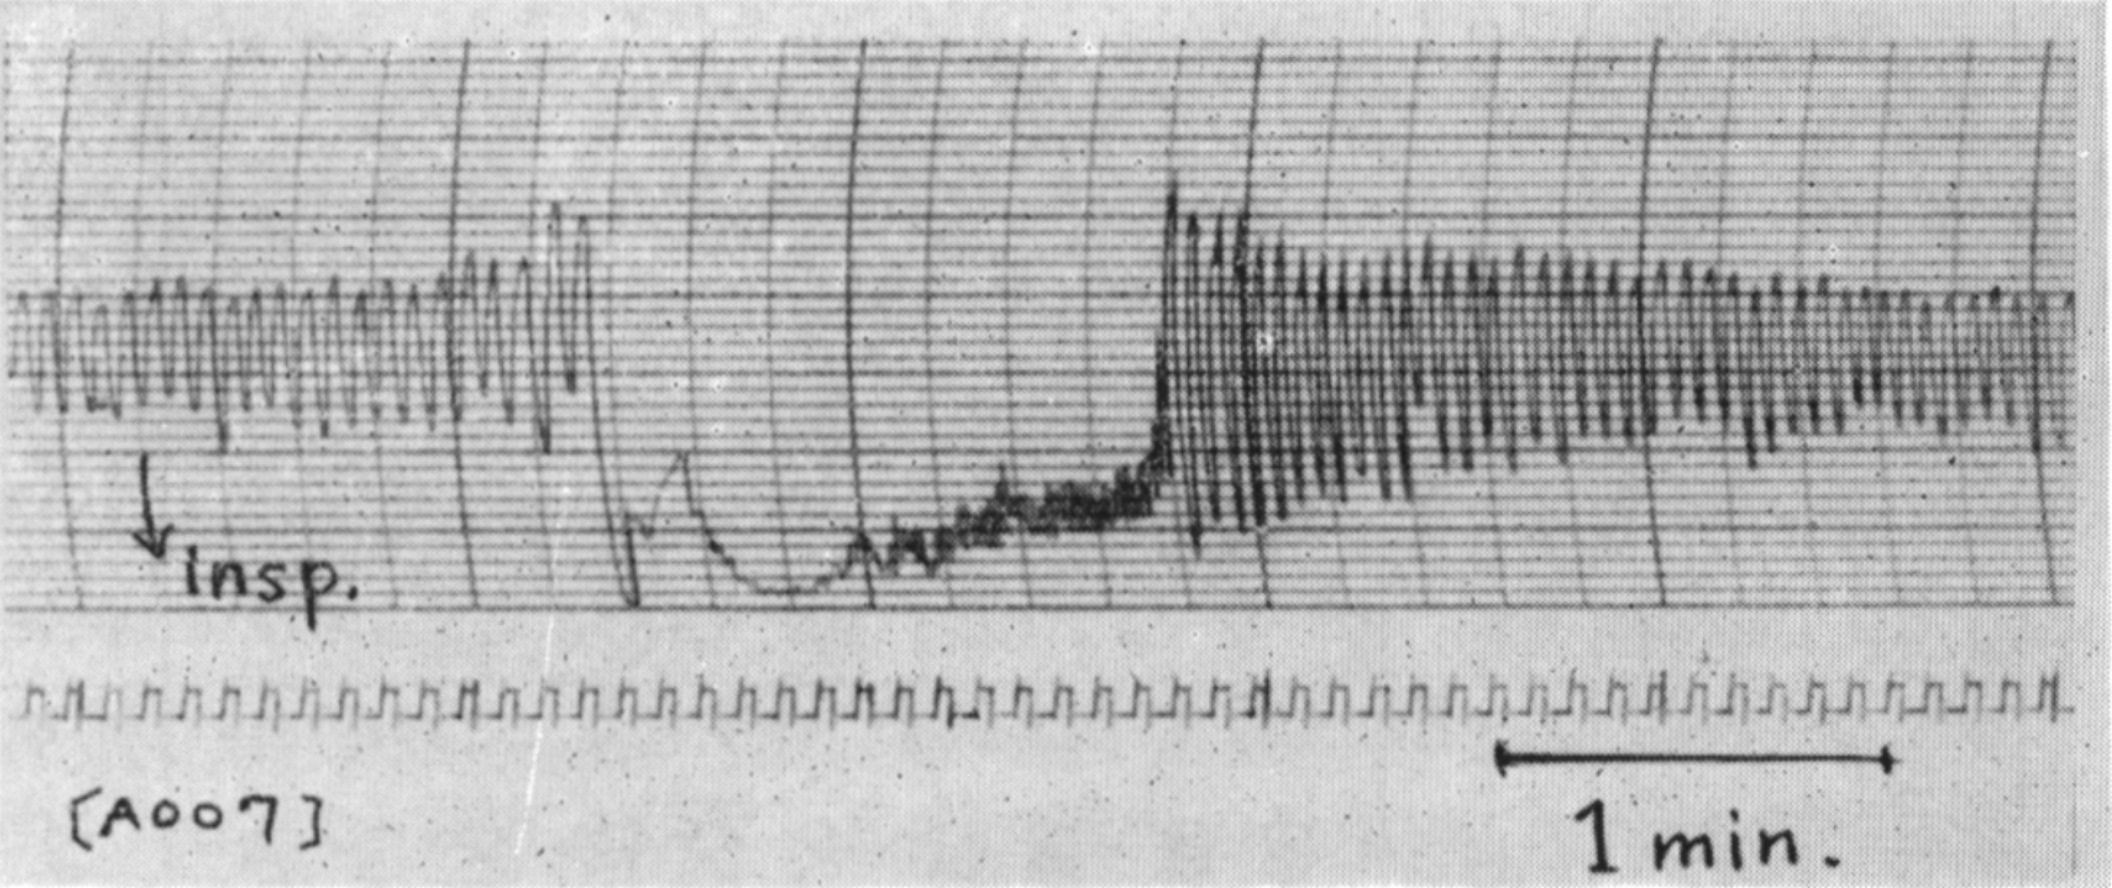
\includegraphics[width=0.66\textwidth]{images/respiration/respiration_regeneration}
    \caption{Regenerationsphase nach dem Luftanhalten \cite{beath_rebreathing}.}
    \label{fig_respiration_regeneration}
\end{figure}

\begin{figure}[ht]
    \centering
    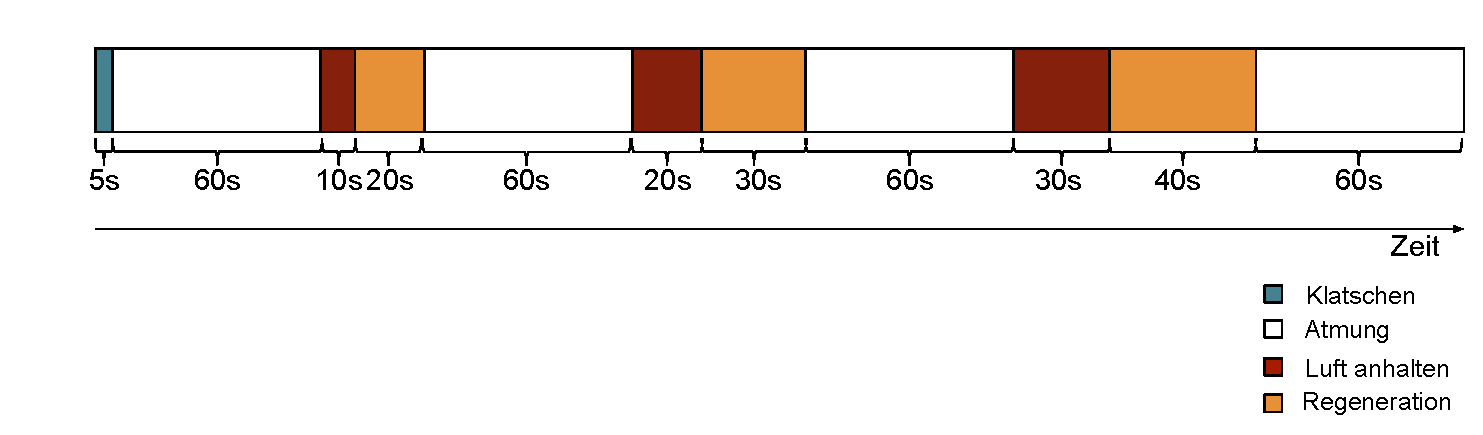
\includegraphics[width=1\textwidth]{images/study/study_flow2}
    \caption{Ablauf der Studie mit einer Position}
    \label{fig_study_flow}
\end{figure}


\section{Systemmodelle}
Zur Datenaufzeichnung während der Studie wurde eine Smartphone-App für Apple-Geräte konzipiert und mit der Sprache Swift entwickelt. 
Mit der Software XCode lässt sich eine mit Swift geschriebene App kompilieren und auf dem Smartphone installieren.

Zur Einbindung externer Frameworks werden die Dependency-Manager \textit{Accio} und \textit{Carthage} verwendet.
Im Folgenden sind die relevanten Frameworks aufgelistet, welche in der App eingebunden worden sind:

\begin{center}
  \begin{tabular}{ | l | l | }
    \hline
    Imperio & Strukturierung der App \\ \hline
    Realm-Cocoa & Datenbank-Framework \\ \hline
    Zip & Bietet die Möglichkeit, einen Ordner \\ 
    & als {\glqq zip\grqq}-Datei zu komprimieren\\ \hline
    Mungohealer & Fügt Logging zu der App hinzu \\
    \hline
  \end{tabular}
\end{center}

Durch das Framework \textit{Imperio} ist es möglich, die View-Komponenten von der Logik zu trennen. 
Somit ändert sich die Struktur der App, indem jeder Ablauf in der App als \textit{Flow} interpretiert wird. 
Pro Flow wird ein \textit{FlowController} angelegt, welcher die Logik des Ablaufs kontrolliert. 
Ein Flow kann nun beliebig viele \textit{ViewController} starten.
Jede \textit{View}, welche von einem Flow aufgerufen wird, hält ein \textit{Delegate} Objekt.
Ein \textit{Delegate} ist ein Protokoll, womit dem \textit{Flow} eine Aktion auf der \textit{View} mitgeteilt werden kann.
Somit wird bei jeder Aktion auf der View eine Funktion des FlowControllers aufgerufen, welcher die View gestartet hat.

\todo{grafik hinzufügen (einfache Grafik anscheinend)}

Das Framework \textit{Realm} ist eine Datenbank für mobile Systeme, die vollständig auf dem mobilen Endgerät läuft.
Die Daten können direkt als \textit{Objekt} ausgelesen und verarbeitet werden.
In der App wird die Datenbank verwendet, um eine Messung abzuspeichern (siehe Abbildung \ref{implementation:app:erModel}))

Das Framework \textit{Mungohealer} stellt eine Möglichkeit dar, bessere Fehlerbenachrichtigungen erstellen zu können. 
Der Standard, welcher von Apple bereitgestellt wird (\textit{NSERROR}), wird durch dieses Framework erweitert.
Somit können Fehler in der Konsole genauer beschrieben werden. 
In dieser App wird dies unter anderem verwendet, um Benachrichtigungen der Bluetoothverbindung zu den eSense-Earpods zu erhalten.     % Entwurf
\chapter{Implementierung}
\label{ch:Implementierung}

In diesem Kapitel wird erläutert, wie die Daten des Datensatzes gesammelt, zur weiteren Verarbeitung vorbereitet und schließlich analysiert werden.
Zur vollständigen Erarbeitung eines Datensatzes muss zuvor eine App erstellt werden, welche die zu sammelnden Daten der eSense-Earpods empfängt und persistiert. 
Zudem soll die App den Ablauf einer Messung automatisch verwalten und danach einen einfachen Export der gespeicherten Daten ermöglichen.
Anschließend müssen die persistierten Daten aufbereitet werden, sodass sie klassifiziert werden können.

\section{App}
\label{ch:Implementierung:app}
Zur Erstellung des Datensatzes wurde eine App entwickelt.
Diese startet eine Messung, nachdem eine Verbindung zu den eSense-Earpods hergestellt wurde.
Jeder Messwert wird in der Datenbank abgespeichert.
In Abbildung \ref{implementation:app:erModel} ist das ER"=Diagramm der Datenbank beschrieben.
Das Gerät wird bei der ersten Kopplung mit dem Namen und dessen Identifikator in der Tabelle {\glqq Device\grqq} abgespeichert.
Der Identifikator ist hierbei eine Repräsentation der MAC-Adresse, welche unter Swift nicht erreichbar ist.
Für jeden Messwert wird ein Eintrag in der Tabelle {\glqq EsenseData\grqq} abgelegt sowie eine Referenz zu den \textit{x-}, \textit{y-} und \textit{z}-Achsenwerten der Gyroskop- und Beschleunigungsdaten, welche in der entsprechenden Tabelle abgelegt werden.
Zudem wird für jede Messung ein Zeitstempel (\texttt{timestamp}), eine Messungs"=ID (\texttt{measurementID}), die aktuell auszuführende Aufgabe (\texttt{task}) und die Information, ob die LED des Smartphones an ist, oder nicht (\texttt{lightOn}), abgespeichert.

Die App ist in 3 Sektionen aufgeteilt, einer \textit{Chartansicht}, einer \textit{Messungsansicht} sowie einer \textit{Einstellungsansicht} (Abb. \ref{implementation:app:screenshots} Tabbar).
Im Weiteren wird nur die \textit{Messungsansicht} genauer erläutert, da die anderen Ansichten im Rahmen der Bachelorarbeit nicht relevant sind.

\begin{figure}[ht]
  \centering
  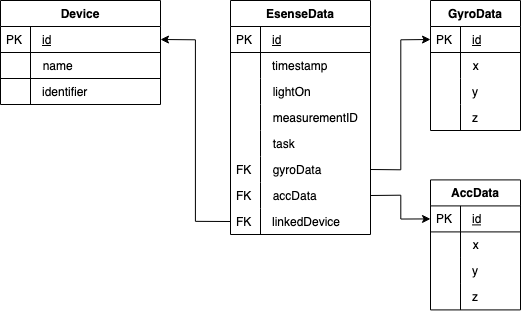
\includegraphics[width=0.7\textwidth]{implementation/app/Database_SleepEar}
  \caption{ER-Diagramm der App-Datenbank}
  \label{implementation:app:erModel}
\end{figure}

\newpage
\subsection{Messungsablauf}
\label{ch:Implementierung:app:measurement_procedure}
Mit der Messungsansicht soll eine komplette Messung durchgeführt werden.
Der \textit{MeasurementFlow} wird gestartet und die erste \textit{View} (Abb. \ref{implementation:app:screenshots:connect_bluetooth}) wird geöffnet.
Nach der erfolgreichen Verbindung mit den eSense-Earpods erfolgt eine Weiterleitung zur nächsten \textit{View} (Abb. \ref{implementation:app:screenshots:user_studies_information}) zum Ausfüllen der Nutzerinformationen. 
Mit dem Betätigen des Buttons {\glqq Start Measurement\grqq} bestätigt man die Eingabe der Daten und die Messung beginnt.
Automatisch startet der erste Timer (Abb. \ref{implementation:app:screenshots:measurement_started}).
Der Timer zeigt den aktuellen, den nächsten \textit{Task} und die Restzeit des aktuellen Tasks an.
Der genaue Ablauf der einzelnen Timer ist in Abbildung \ref{fig_study_flow} detailliert beschrieben.
Nach dem Ablauf des letzten Timers wird eine View geöffnet, welche die Möglichkeit zum Teilen der aktuellen Messung bietet (Abb. \ref{implementation:app:screenshots:sampling_stopped}, \ref{implementation:app:screenshots:share}).
Zudem kann die Datenbank vollständig geleert werden.
Während dieses Ablaufs wird ein Objekt erstellt, welches die Messung verwaltet.

\subsection{Messung}
\label{ch:Implementierung:app:measurement}
Eine Messung wird im Code in einem \textit{Measurement} Objekt persistiert.
Durch ein Observer-Pattern wird der \textit{MeasurementFlow} über jegliche Änderung informiert und kann entsprechende Handlungen durchführen.
Durch die Funktionen \texttt{startMeasurement} und \texttt{stopMeasurement} kann eine Messung gestartet beziehungsweise gestoppt werden.
Mit der Funktion \texttt{startMeasurement} wird das IMU-Sampling per BLE sowie die Audioaufnahme gestartet. 
Ebenso wird der erste Timer gestartet und ein doppeltes Lichtsignal wird gesendet. 
Durch die Funktion \texttt{stopMeasurement} werden die Datenströme gestoppt, ebenfalls ein doppeltes Lichtsignal gesendet und der Timer wird beendet.
Der nächste Task wird gestartet, wenn der Timer abgelaufen ist. Der Timer startet mit der Länge des nächsten Tasks.
Sofern der nächste Task {\glqq \textit{Hold\_breath}\grqq} ist, also die Person im folgenden Task die Luft anhält, wird dem Teilnehmer kurz vor Ablauf mitgeteilt, wann der nächste Task startet.
Mit der Instruktion \glqq Bitte die Luft anhalten in 3, 2, 1\grqq \ weiß der Teilnehmer, wann er die Luft anhalten soll.
Durch die Anweisung \glqq Stopp\grqq \ wird dem Nutzer das Ende des Tasks mitgeteilt. 
Die Instruktionen liegen als Audiodatei vor und werden jeweils vor dem jeweiligen Task abgespielt und mittels Bluetooth über die Lautsprecher der eSense-Earpods ausgegeben.

\newpage
\section{Anbindung an die Auswertungspipeline}
\label{ch:Implementierung:way_to_pipeline}
\begin{wrapfigure}{r}{0.3\textwidth}
  \centering
  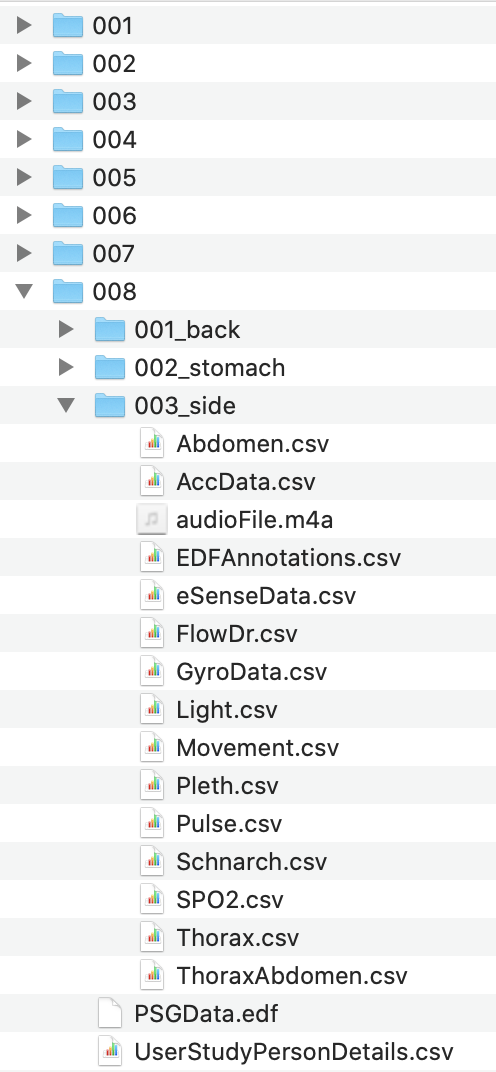
\includegraphics[width=0.25\textwidth]{data_analyzation/folder_structure}
  \caption{Ordnerstruktur des Datensatzes}
  \label{implementation:folder_structure}
\end{wrapfigure}
Die App liefert beim Export die Daten der eSense-Earpods.
Diese beinhalten die IMU-Daten, die Nutzer"-informationen und die Mikrofonaufnahme.
Zum aktuellen Stand liegen somit die Daten der eSense-Earpods und die des PSG-Systems vor. 
Zu Beginn müssen die PSG-Daten, welche als eine Messung für alle 3 Positionen pro Studienteilnehmer persistiert wurde, in 3 einzelne Mes"-sungen aufgeteilt werden.
Die Daten des PSG-Systems liegen als \textit{edf}-Datei vor. 
Diese können mittels Python und der Library \texttt{edfrd} ausgelesen werden.
Jedoch sind die Einträge des jeweiligen Signals ohne einen Zeitwert abgespeichert. 
Es muss nun aufgrund der Abtastrate in $\si{\hertz}$ die Zeit manuell berechnet werden. 
Mittels der Funktion \texttt{find\_peaks} aus \texttt{scipy.peak}\ können die Peaks des Lichtsensors am PSG-System ermittelt werden (siehe Abb. \ref{implementation:synchronisation:peaks_psg}).
Da eine Messung mit 2 Lichtblitzen beginnt und endet, kann nun der Start- und Endzeitpunkt einer Position ermittelt werden. 
Die einzelnen Positionen können dadurch voneinander unterschieden werden. 
Daraufhin können die 11 verfügbaren Signale einzeln ausgelesen werden.
Pro Position wird nun jedes der Signale als \textit{csv}-Datei im jeweiligen Ordner abgelegt.
Die Daten der eSense-Earpods liegen getrennt in \newline \textit{AccData\_\$ID\$.csv} und \textit{GyroData\_\$ID\$.csv} vor. 
Diese werden ausgelesen und zu der Datei \textit{eSenseData.csv} zusammengeführt.
Die Ordnerstruktur kann der Abbildung \ref{implementation:folder_structure} entnommen werden und ist nun vollständig.

\begin{figure}[ht]
  \centering
  \begin{subfigure}{.25\textwidth}
    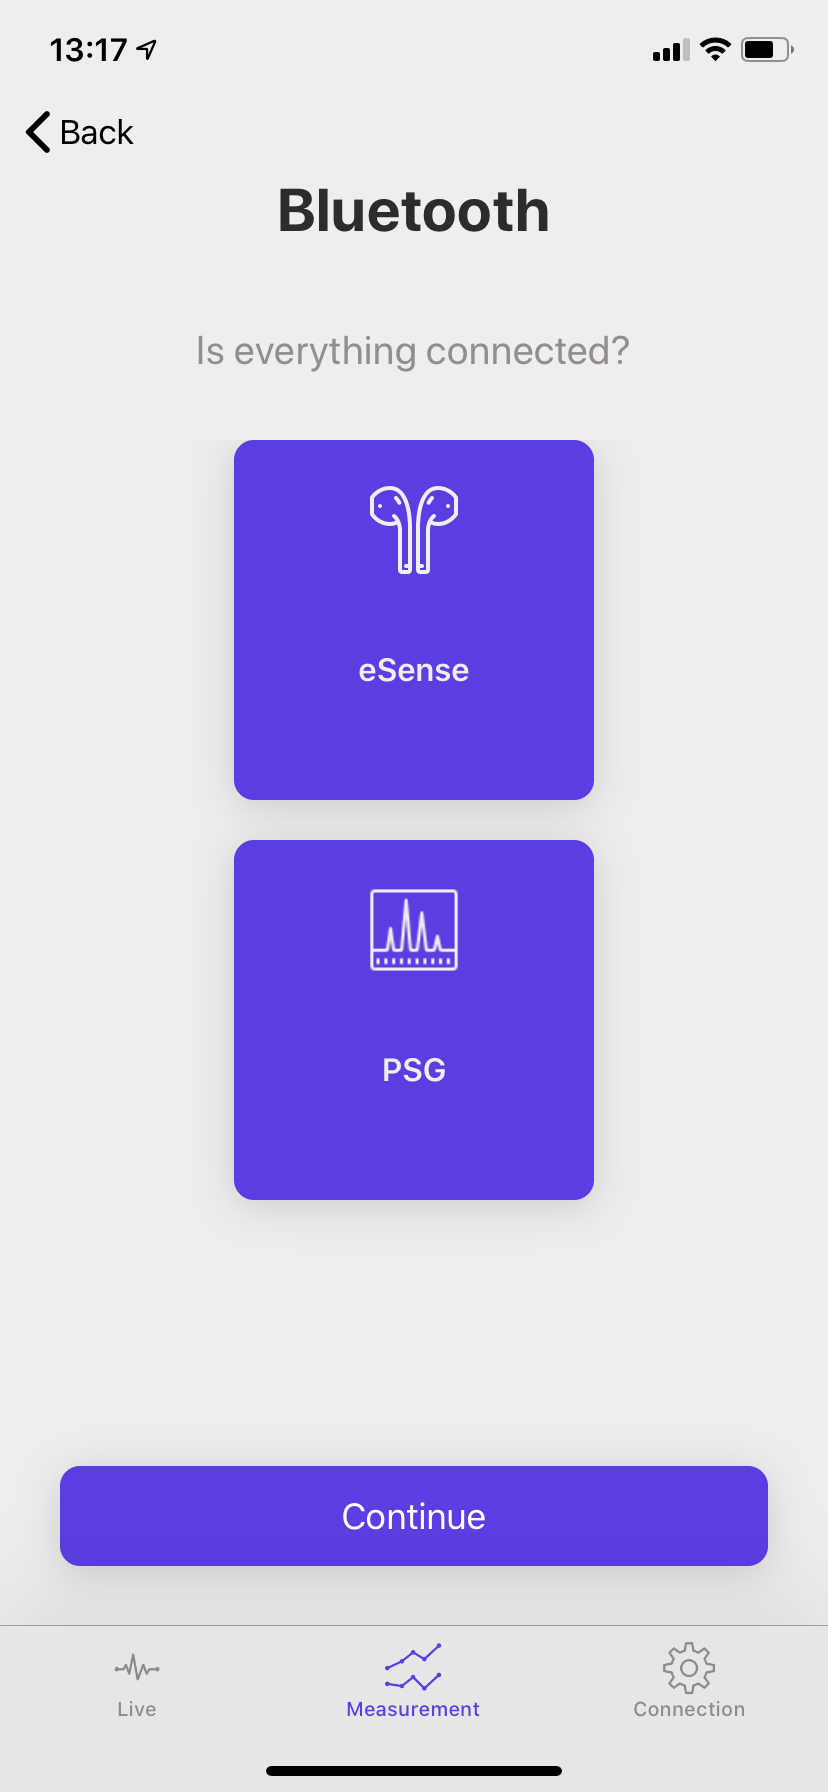
\includegraphics[width=1\textwidth]{app/connect}
    \caption{Verbinden der eSense-Earpods}
    \label{implementation:app:screenshots:connect_bluetooth}
  \end{subfigure}
  \begin{subfigure}{.25\textwidth}
    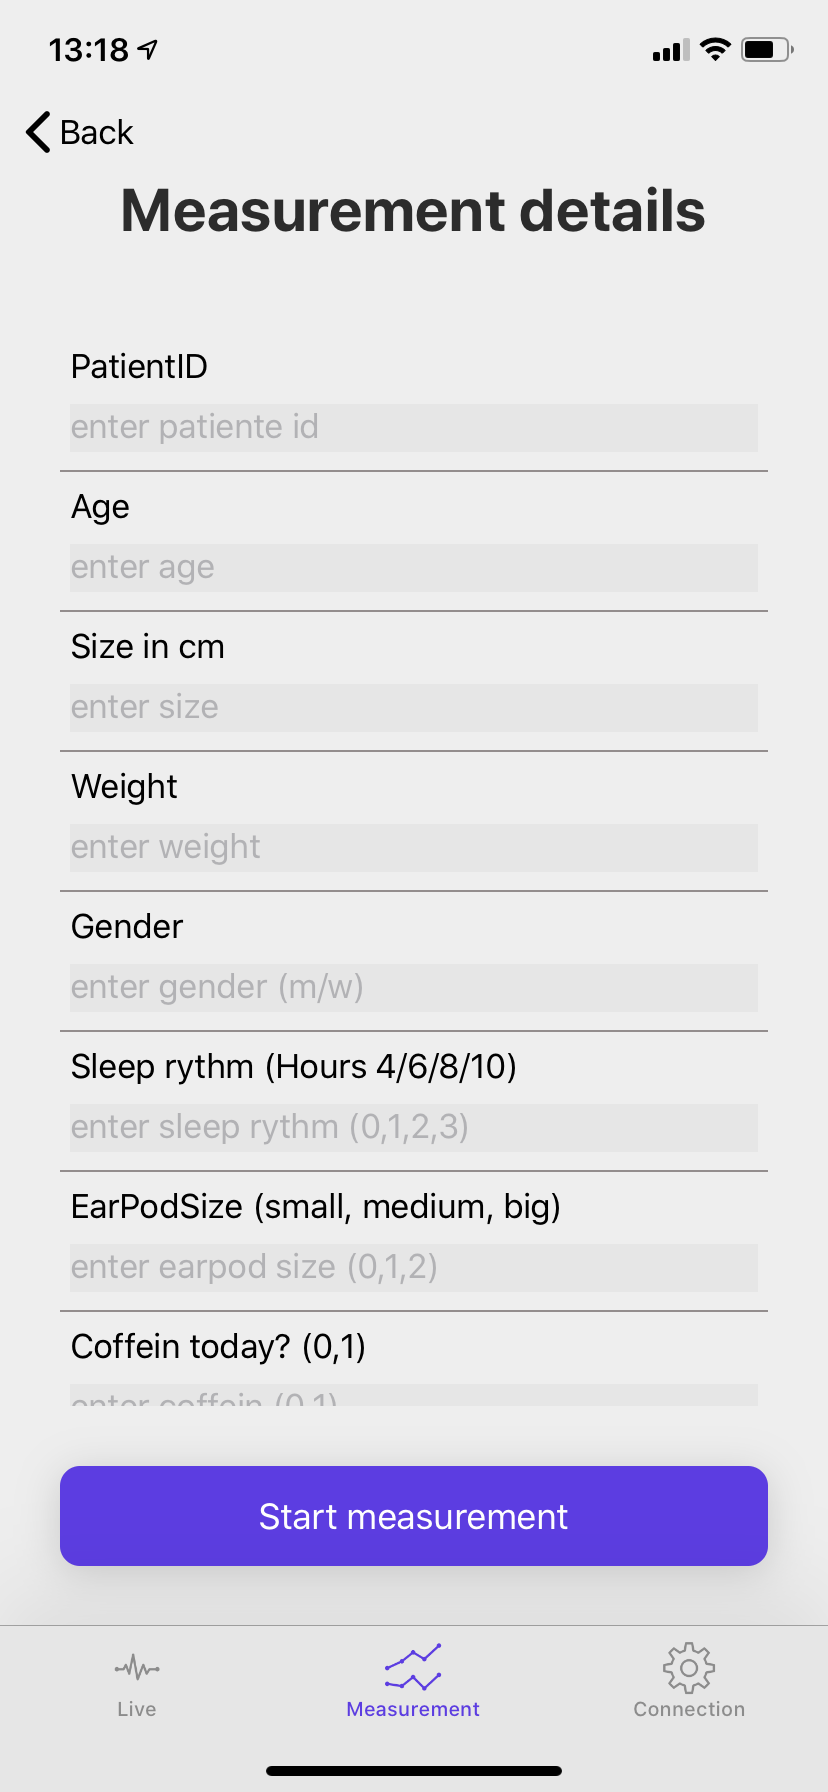
\includegraphics[width=1\textwidth]{app/measurement_details}
    \caption{Eingabe der Nutzerinformationen}
    \label{implementation:app:screenshots:user_studies_information}
  \end{subfigure}
  \begin{subfigure}{.25\textwidth}
    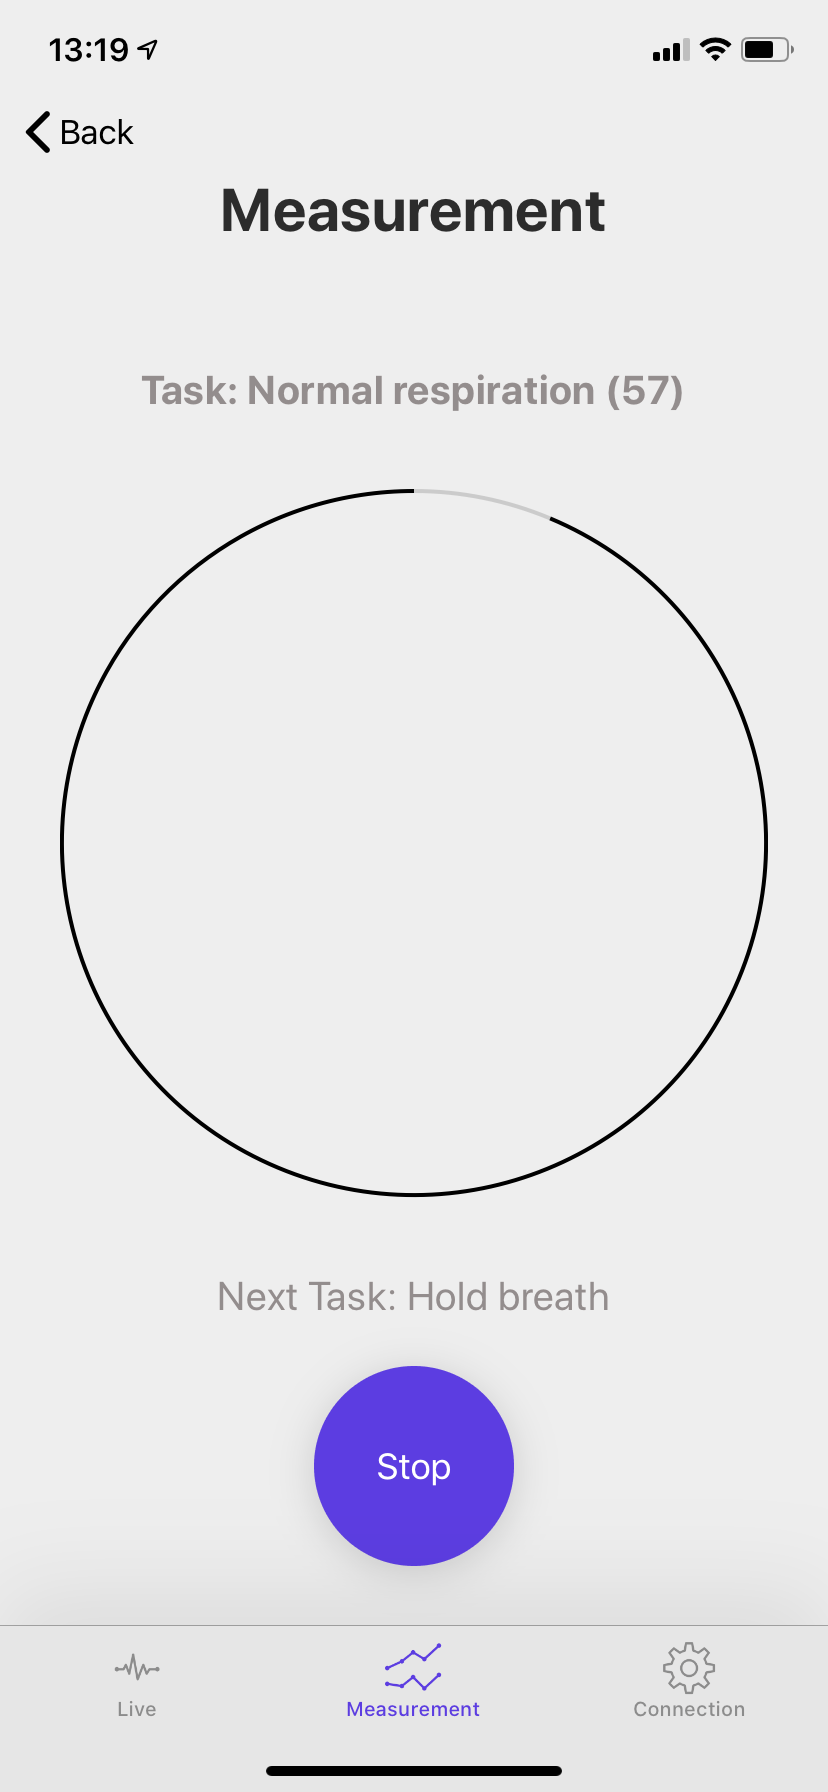
\includegraphics[width=1\textwidth]{app/measurement_timer_02}
    \caption{Messung, aktueller und nächster Task}
    \label{implementation:app:screenshots:measurement_started}
  \end{subfigure}
  \begin{subfigure}{.25\textwidth}
    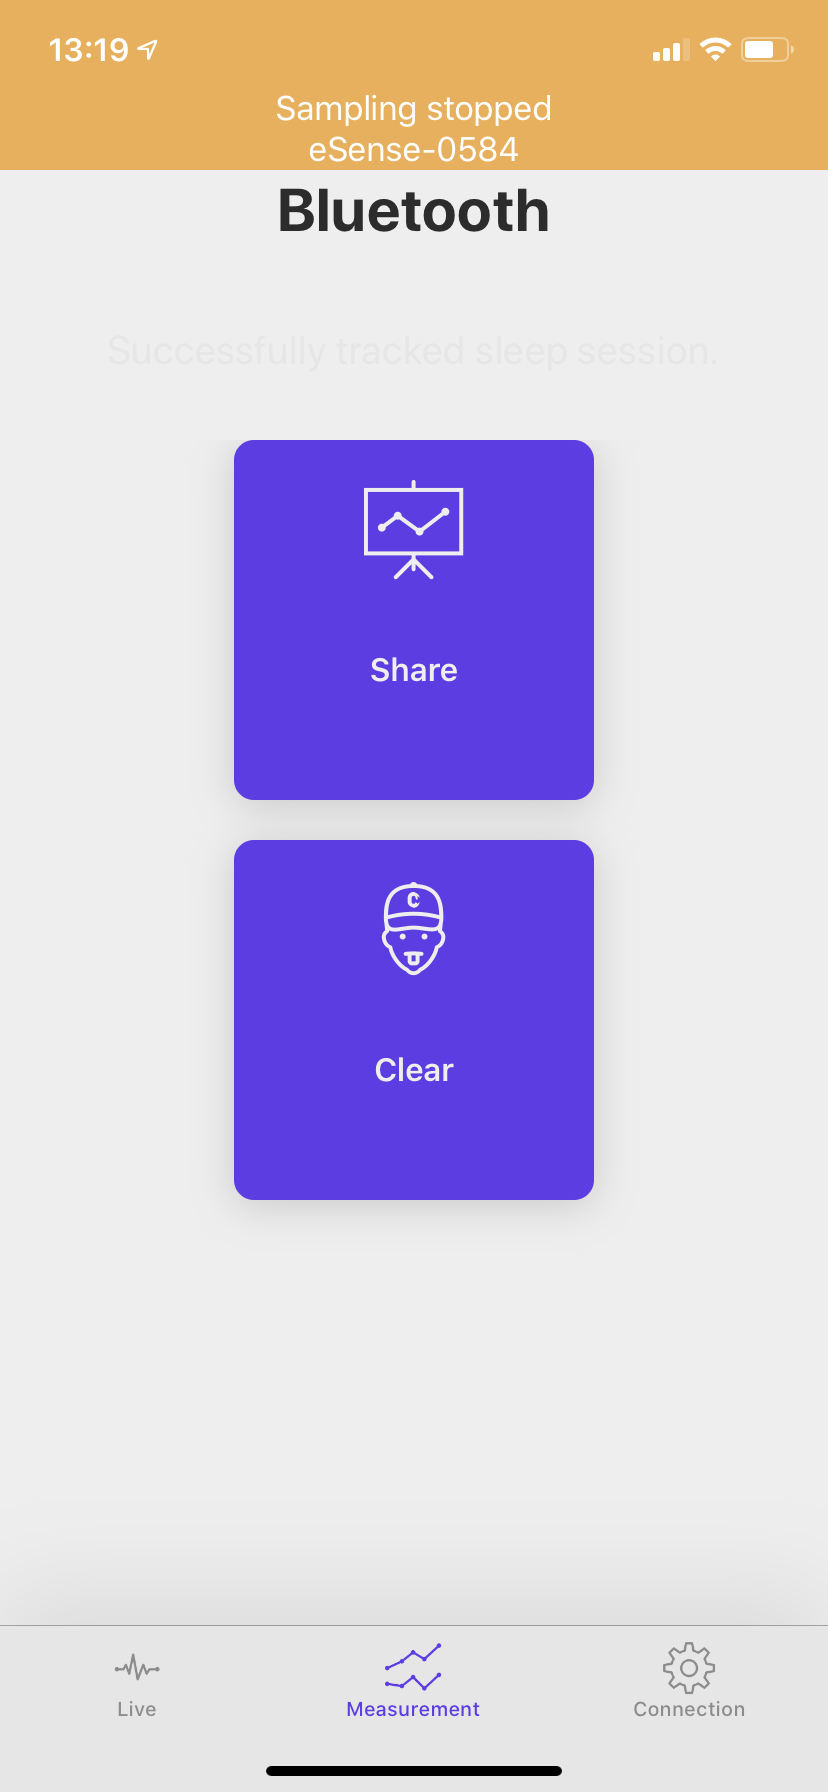
\includegraphics[width=1\textwidth]{app/measurement_finished}
    \caption{Messung beendet}
    \label{implementation:app:screenshots:sampling_stopped}
  \end{subfigure}
  \begin{subfigure}{.25\textwidth}
    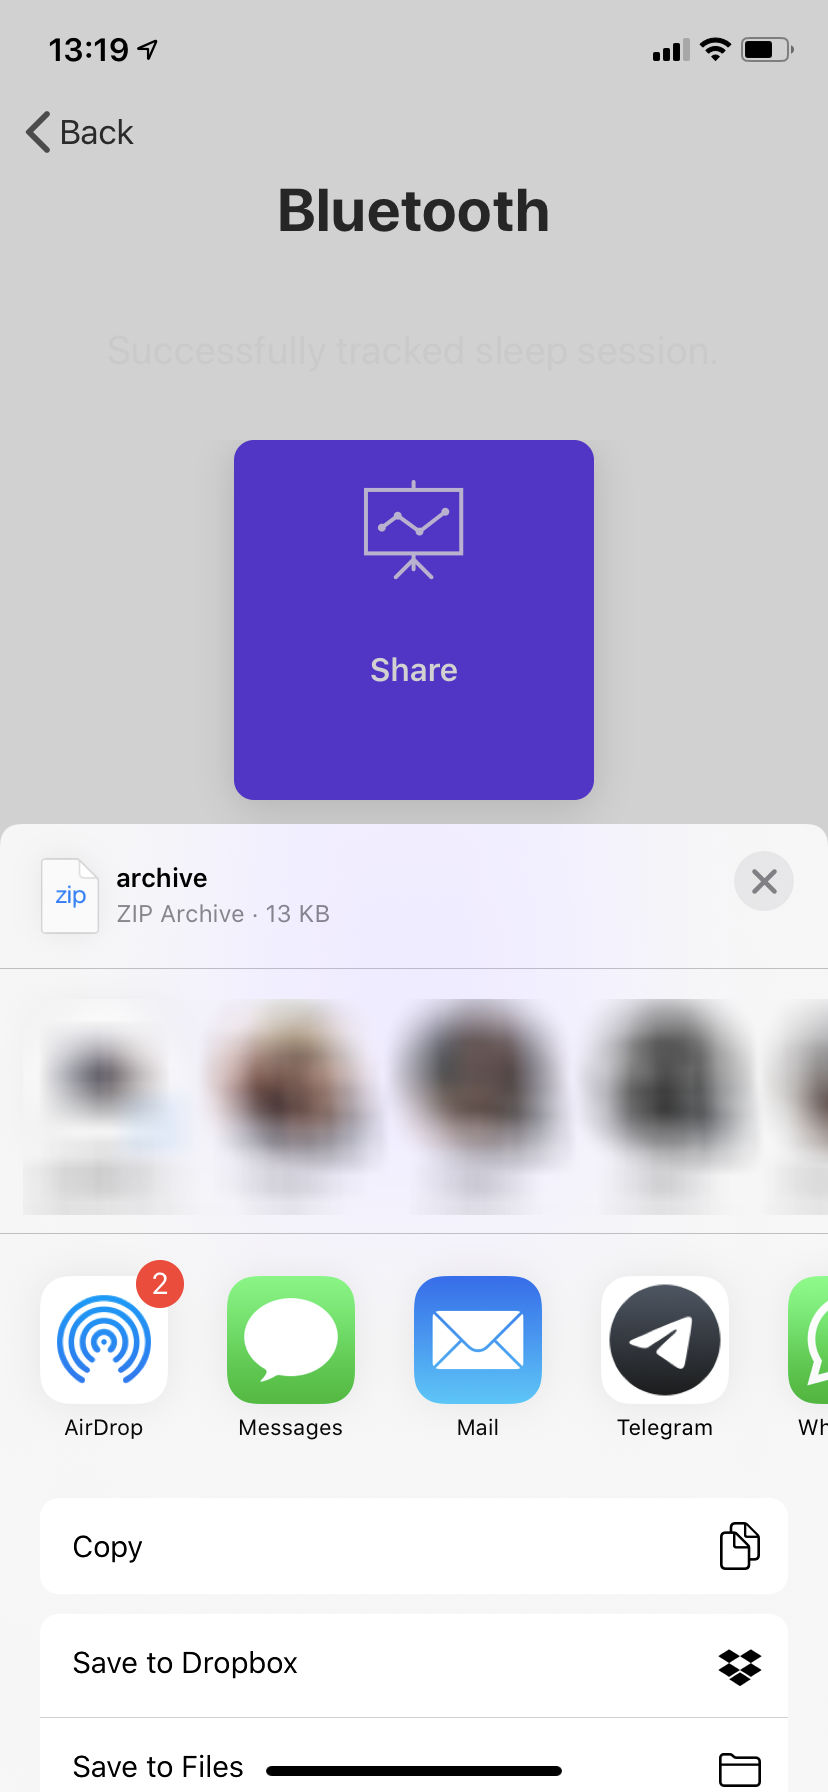
\includegraphics[width=1\textwidth]{app/measurement_share}
    \caption{Messung teilen}
    \label{implementation:app:screenshots:share}
  \end{subfigure}
  \caption{Verlauf einer Messung mit der App: Zu Beginn wird eine Verbindung mit den eSense-Earpods hergestellt. Anschließend werden die Nutzerinformationen des Probanden abgefragt. Mit dem Klick auf \textit{Start Measurement} wird eine Messung gestartet. Der erste Timer läuft ab und über die Lautsprecher werden alle Informationen an den Probanden weitergegeben. Nach Ablauf des Timers beginnt der nächste Timer. Sobald der letzte Timer abgelaufen ist, kann die Messung geteilt werden. Zudem kann die Datenbank gelöscht werden und die nächste Messung kann beginnen. Der Ablauf einer Messung ist in Abbildung \ref{fig_study_flow} zu sehen.}
  \label{implementation:app:screenshots}
\end{figure}

\subsection{Synchronisation der Daten}
\label{ch:Implementierung:data_sync}
Da es nicht garantiert ist, dass der Timer des PSG-Systems zuverlässig arbeitet, wird jeder Peak des Lichtsensors mit dem Lichtsignal der Smartphone-Daten verglichen.
Der Abstand jedes einzelnen Peaks wird nun ermittelt, ebenso wie die durchschnittliche Distanz der Peaks.
In der Abbildung \ref{implementation:synchronisation:before_light_peak} ist der Vergleich eines Lichtblitzes vom Smartphone (blau) und dem PSG-System (orange) im zeitlichen Verlauf dargestellt (\texttt{time}).
Da die Verschiebung des Timers des PSG-Systems während einer 7-minütigen Messung im Mittel bei $0.3\si{\s}$ lag, wurde der Timer des PSG-Systems um die durchschnittliche Distanz der Peaks verschoben.
Dies ist ausreichend, da die PSG-Daten in der Bachelorarbeit lediglich dem visuellen Vergleich dienen und in der Klassifikation nicht mitbetrachtet werden. 
Die zeitliche Verschiebung wird nun in jede \textit{csv}-Datei mit der Spalte \texttt{new\_time} eingearbeitet.
In Abbildung \ref{implementation:synchronisation:after_light_peak} ist klar zu erkennen, dass mit dem neuen Zeitwert (\texttt{new\_time}) der Lichtwert des PSG-Signals (orange) direkt über dem Lichtwert des Smartphonesignals (blau) liegt.
Nun ist garantiert, dass die Zeitwerte des PSG-Systems und des Smartphones synchron sind. Die Daten sind nun bereit zur Analyse.

\begin{figure}[ht]
  \centering
  \begin{subfigure}{0.66\textwidth}
    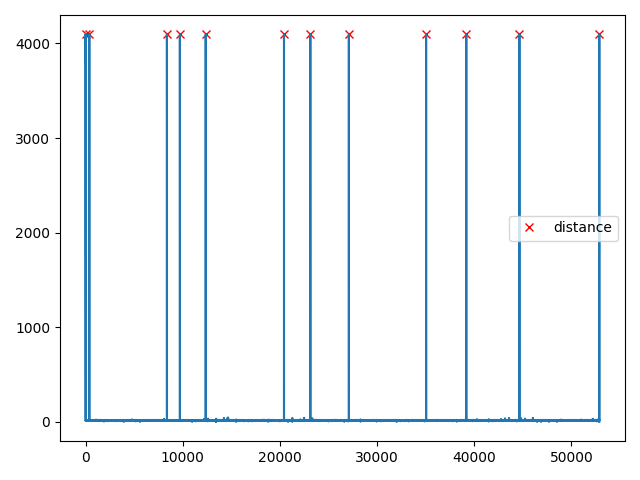
\includegraphics[width=1\textwidth]{data_analyzation/light_peak_detection_psg_data}
    \caption{Peaks des Lichtsignals vom PSG-Gerät. Somit können die PSG-Daten und die von den eSense-Earpods gesammelten Daten zeitlich synchronisiert werden. Das Vorkommen der Lichtpeaks ist identisch zum Ablauf der Nutzerstudie (siehe Abb. \ref{fig_study_flow}). Die y-Achse zeigt den Lichtausschlag des Sensors, die x-Achse den Zeitwert.}
    \label{implementation:synchronisation:peaks_psg}
  \end{subfigure}
  \begin{subfigure}{.49\textwidth}
    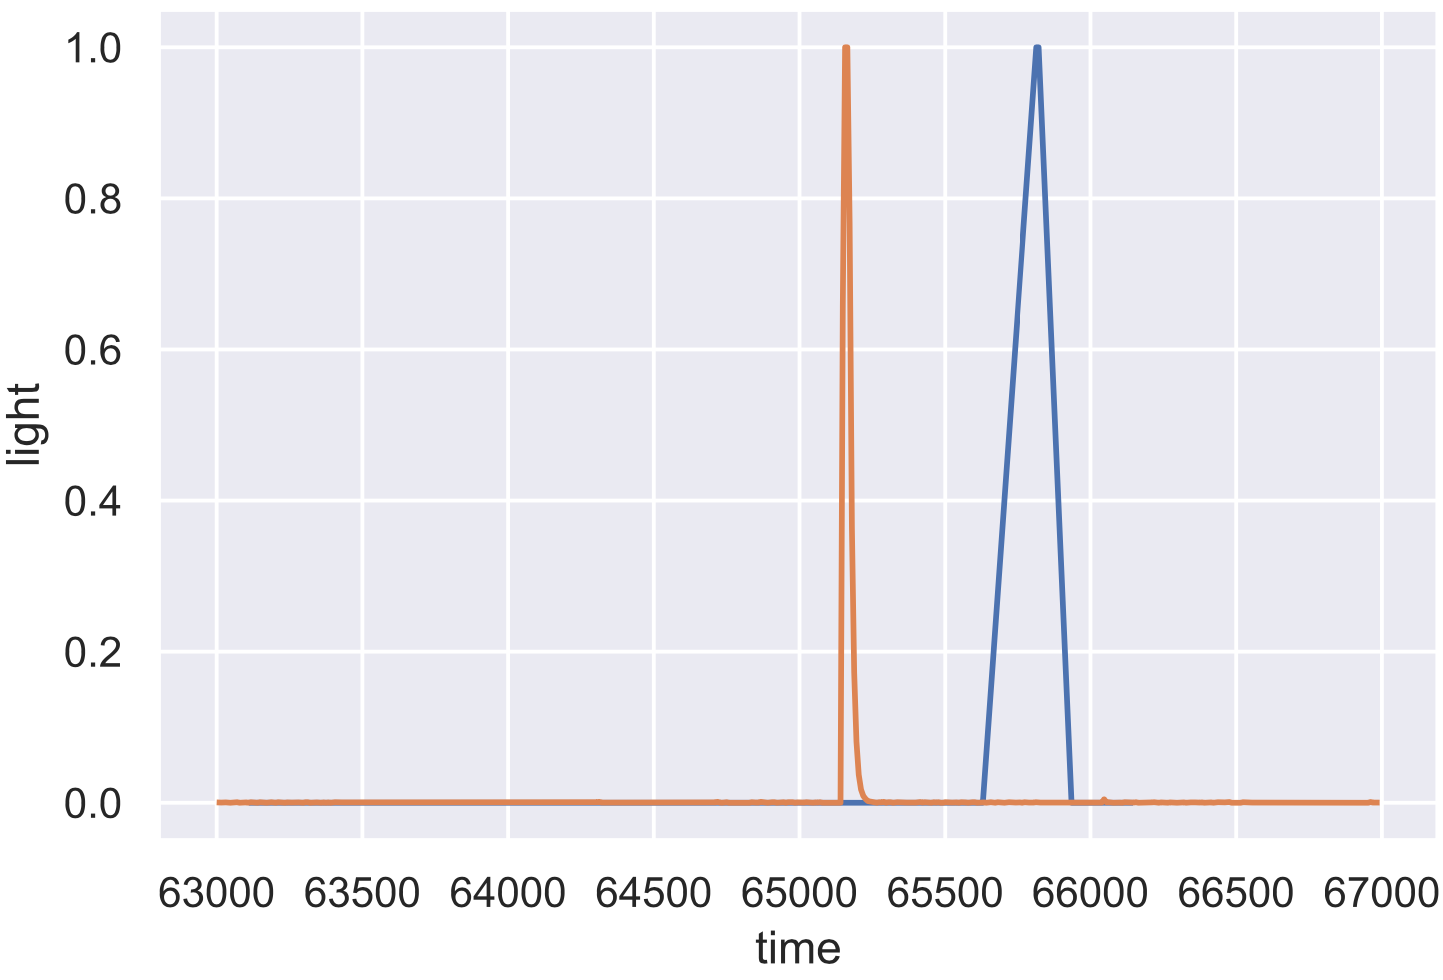
\includegraphics[width=1\textwidth]{data_analyzation/light_peak_detail_before.png}
    \caption{Zeitlicher Lichtpeakvergleich vor der Synchronisation. Der Lichtpeak des PSG-Geräts (orange) ist weniger als 1s vom Signal der eSense-Earpods (blau) entfernt. Der Zeitwert ist in $\si{\ms}$ angegeben. Die Lichtsignale wurden skaliert, um diese vergleichen zu können. }
    \label{implementation:synchronisation:before_light_peak}
  \end{subfigure}
  \begin{subfigure}{.49\textwidth}
    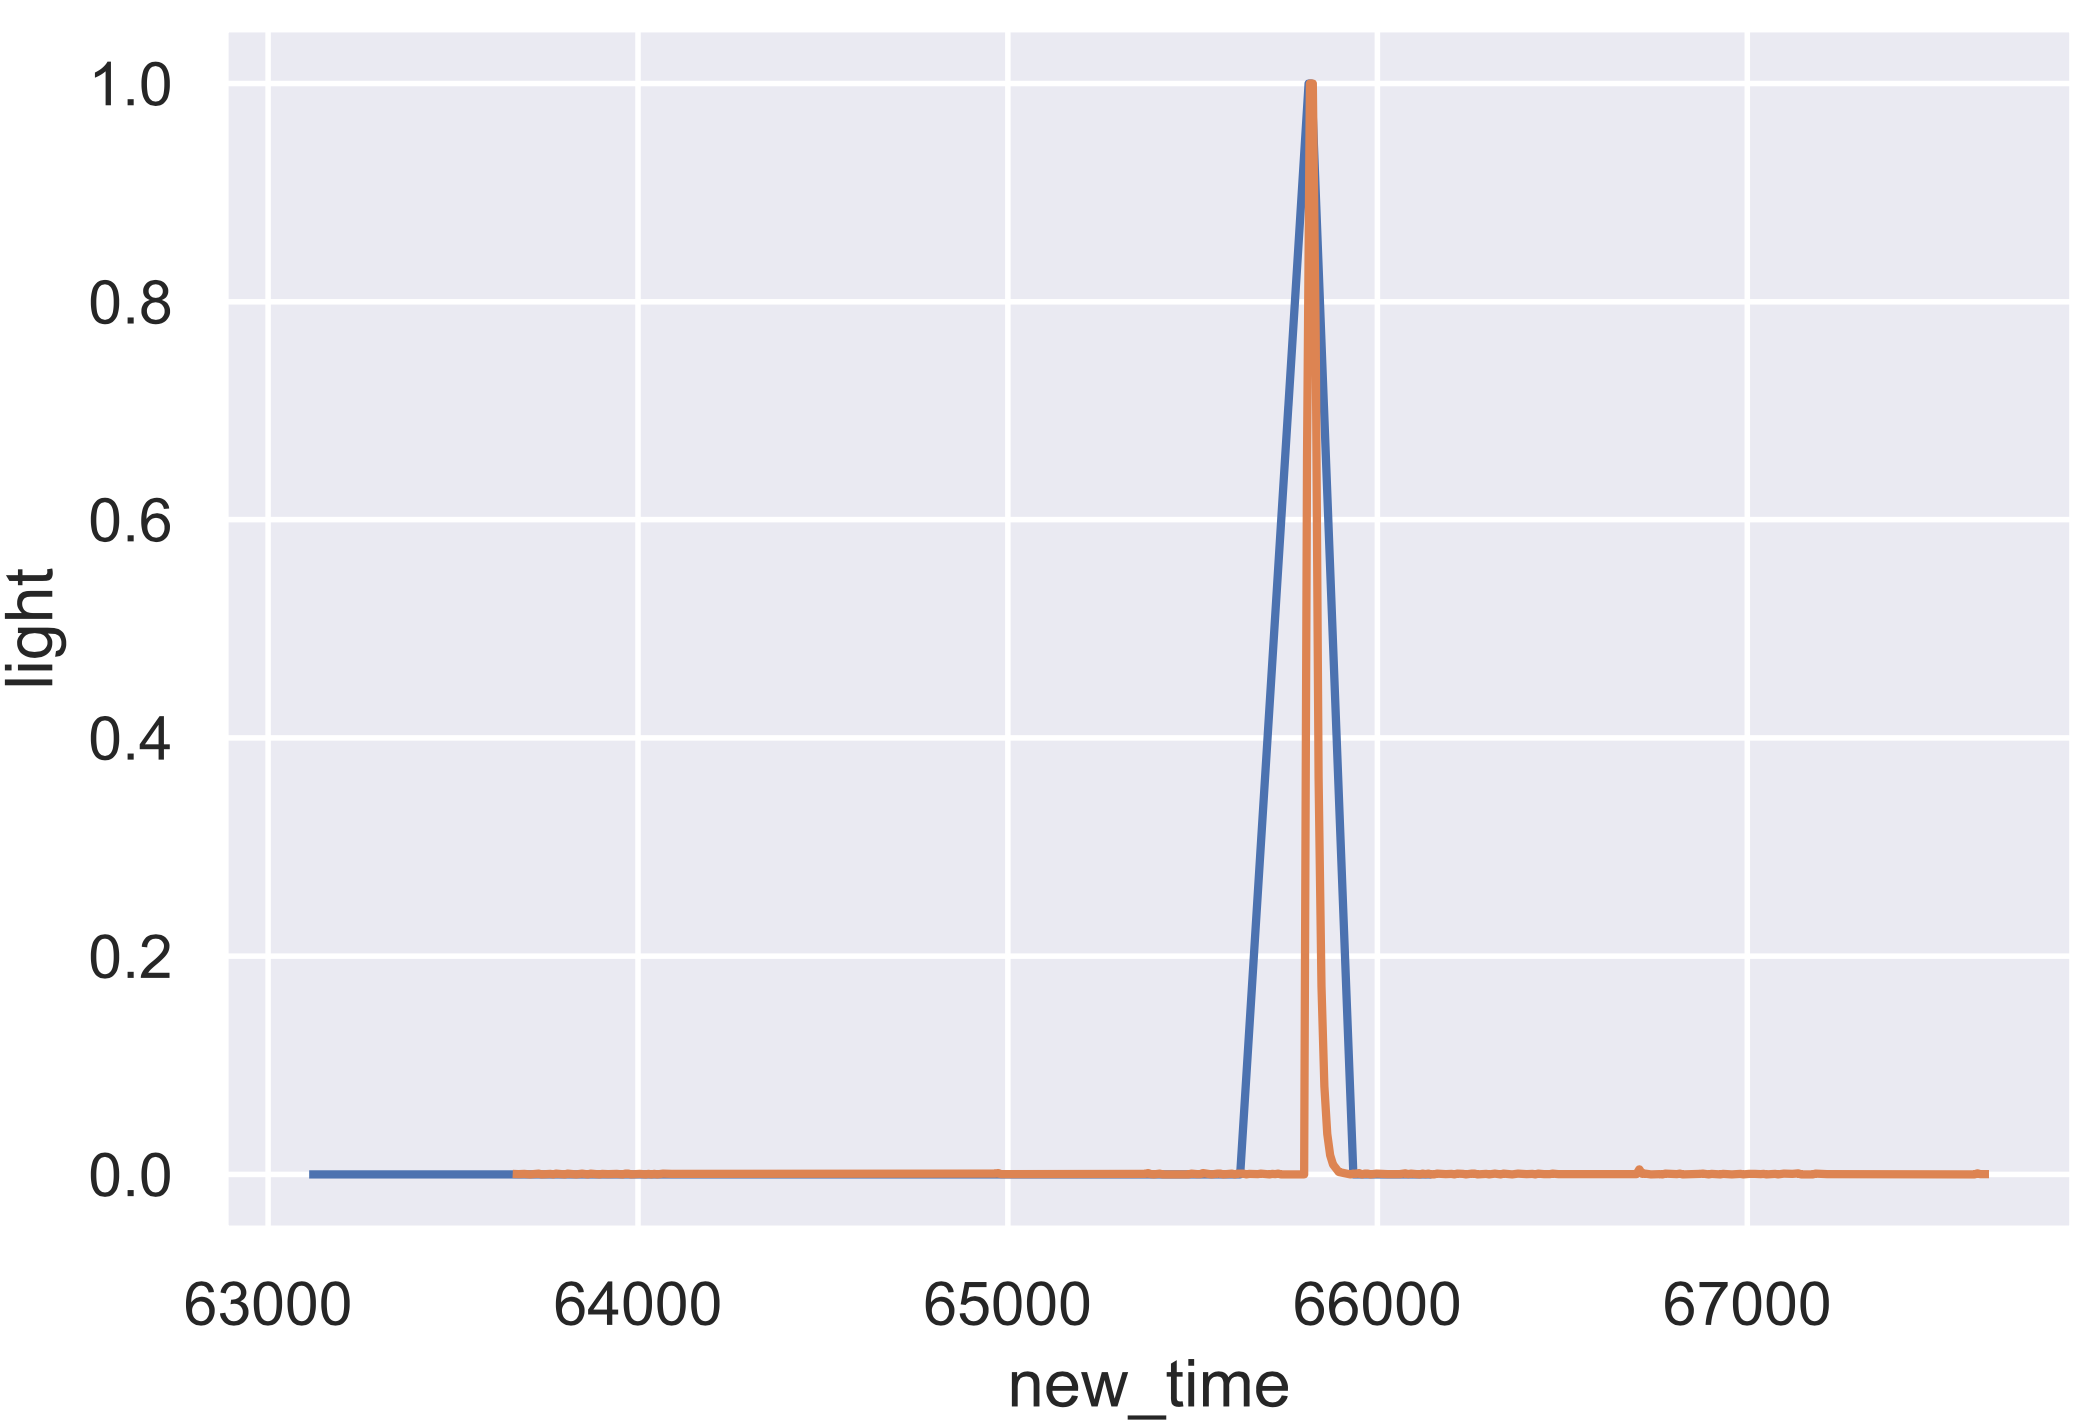
\includegraphics[width=1\textwidth]{data_analyzation/light_peak_detail_after.png}
    \caption{Zeitlicher Lichtpeakvergleich nach der Synchronisation. Der Lichtpeak des PSG-Systems (orange) ist nun zeitlich sehr nahe über den Lichtpeaks der eSense-Earpods (blau). Der neue Zeitwert ist in der Spalte \texttt{new\_time} jeder Datei zu entnehmen. Der Zeitwert ist in $\si{\ms}$ angegeben.}
    \label{implementation:synchronisation:after_light_peak}
  \end{subfigure}
  \caption{Synchronisation der Lichtpeaks: Die Signale des PSG-Geräts müssen mit denen der eSense-Earpods zeitlich synchronisiert werden, damit diese zeitlich vergleichbar sind.}
  \label{implementation:synchronisation:peaks}
\end{figure}

\newpage
\section{Verarbeitungspipeline zur Klassifikation}
\label{ch:Implementierung:classification_pipeline}
Zur Klassifizierung der Daten müssen nun Features berechnet werden. 
Diese werden jedoch nicht auf das ganze Zeitintervall einer Messung berechnet, sondern aufgeteilt.
Eine Messung wird nun in Fenster der Größe von 5 bzw. 10 Sekunden aufgeteilt, wobei jedes Fenster um eine Sekunde verschoben wird. 
Somit überlappen sich zwei aneinander grenzende Fenster immer um 4 bzw. 9 Sekunden. 
Die Trennung der Fenster wurde anhand des Zeitwertes jedes Messergebnisses entschieden, da die Messergebnisse der eSense-Earpods beim Senden per BLE an das Smartphone keine Uhrzeit beinhalten.
Dadurch liegt kein genauer Abstand der einzelnen Messdaten von $50\si{\hertz}$ vor. 
Anschließend wurden mittels des Moduls \texttt{tsfresh} Features für jedes Fenster einzeln berechnet und es entstand eine Datei \textit{df\$patient\_id\$\_\$position\_id\$\_feature.csv}, welche alle Features der einzelnen Fenster beinhaltet.

Da nun die Features für eine Fenstergröße von $5\si{\s}$ und $10\si{\s}$ mit der Verschiebung von $1\si{\s}$ pro Fenster vorliegen, kann mit der Klassifikation begonnen werden.    % Implementierung
%% eval.tex
%% $Id: eval.tex 5 2005-10-10 20:55:48Z bless $

\chapter{Evaluation}
\label{ch:Evaluation}

Zu Beginn der Evaluation wurde eine Nutzerstudie durchgeführt, womit ein Datensatz generiert wurde. 
Anhand dieses Datensatzes wird anschließend ein Klassifikationsmodell erstellt, womit eine Vorhersage darüber getroffen wird, an welcher Stelle ein Apnoeereignis stattgefunden hat.

\section{Studienablauf}
In Kapitel \ref{ch:Design:sec:studienplanung} wurde eine einzelne Messung einer Studie detailliert beschrieben.
Es wurden nun 7 Probanden nach dem Prinzip des \textit{Sample of Convenience} ausgewählt.

Dieser Ablauf (siehe Abb. \ref{fig_study_flow}) wurde nun pro Studienteilnehmer jeweils in den 3 Positionen durchgeführt, womit fast alle Schlaflagen abgedeckt sind.
Zu Beginn der Studie fand eine kurze Einweisung statt, bei der der Proband erfuhr, was er zu tragen hat und wie er Anweisungen erhält, um dem Ablauf folgen zu können. 
Die Kamera wurde auf dem Stativ platziert und so ausgelegt, dass sie das Ohr des Probanden filmt. 
Das PSG-System wurde am Studienteilnehmer angebracht sowie alle nötigen Sensoren, die im Kapitel \ref{ch:sa:psg} beschrieben wurden.
Nachdem die passenden eSense-Earpodaufsätze gefunden wurden, war der Aufbau der Studie beendet.

Nun wurde die Messung des PSG-Systems gestartet, sowie die Smartphone-App geöffnet. 
Nach Eingabe der Nutzerinformationen kann der erste Durchgang, welcher abhängig vom Ablauf der 3 Positionen war, begonnen werden.
Durch den Start der Messung am Smartphone beginnt die Messung. 
Da zusätzlich der Ton durch das Mikrofon am eSense-Earpod mit aufgezeichnet wird, wird nach dem Start der Messung ein $4\si{\s}$ Zeitfenster gewählt, in dem der Teilnehmer in die Hände klatschen muss, um das Mikrofonsignal später synchronisieren zu können.
Nun beginnt die Aufzeichnung. Der Leiter der Studie hat bereits den Raum verlassen und alle Anweisungen werden durch die Earpods per Audiosignal ausgesprochen. 
Sofern die Messung beendet ist, tritt der Leiter der Studie wieder in den Raum und die Messung kann exportiert werden. 
Der Export beinhaltet jegliche Smartphone-Daten. Die PSG-Daten werden als eine komplette Messung am Ende der Studie exportiert.
Zudem wird die Kamera angehalten und eine neue Aufnahme kann gestartet werden.
Anschließend beginnt die nächste Position. Der Proband kann nun die neue Position einnehmen, anschließend wird per App die neue Messung gestartet.
Zum Abschluss aller 3 Positionen wird die Messung am PSG-System gestoppt und mittels eines vom PSG-System bereitgestellten Programms lässt sich die Messung als {\glqq \textit{edf}-Datei\grqq} exportieren.
Weitere Informationen zum Export der Daten und zur Synchronisation sind in Kapitel \ref{ch:Implementierung:way_to_pipeline} zu finden.
Pro Position dauert eine Messung ca. 7 Minuten, was bei 3 Personen eine Gesamtdauer von 21 Minuten bedeutet.
Einschließlich der Instruktionszeit, dem Export nach der Messung und den Positionswechseln der Probanden beträgt die durchschnittliche Gesamtdauer einer Aufzeichnung circa 45-60 Minuten. 

\begin{figure}[ht]
    \centering
    \begin{subfigure}{0.53\textwidth}
        \includegraphics[width=1\textwidth]{study/study_proband_2_clean.png}
    \end{subfigure}
    \begin{subfigure}{0.3\textwidth}
        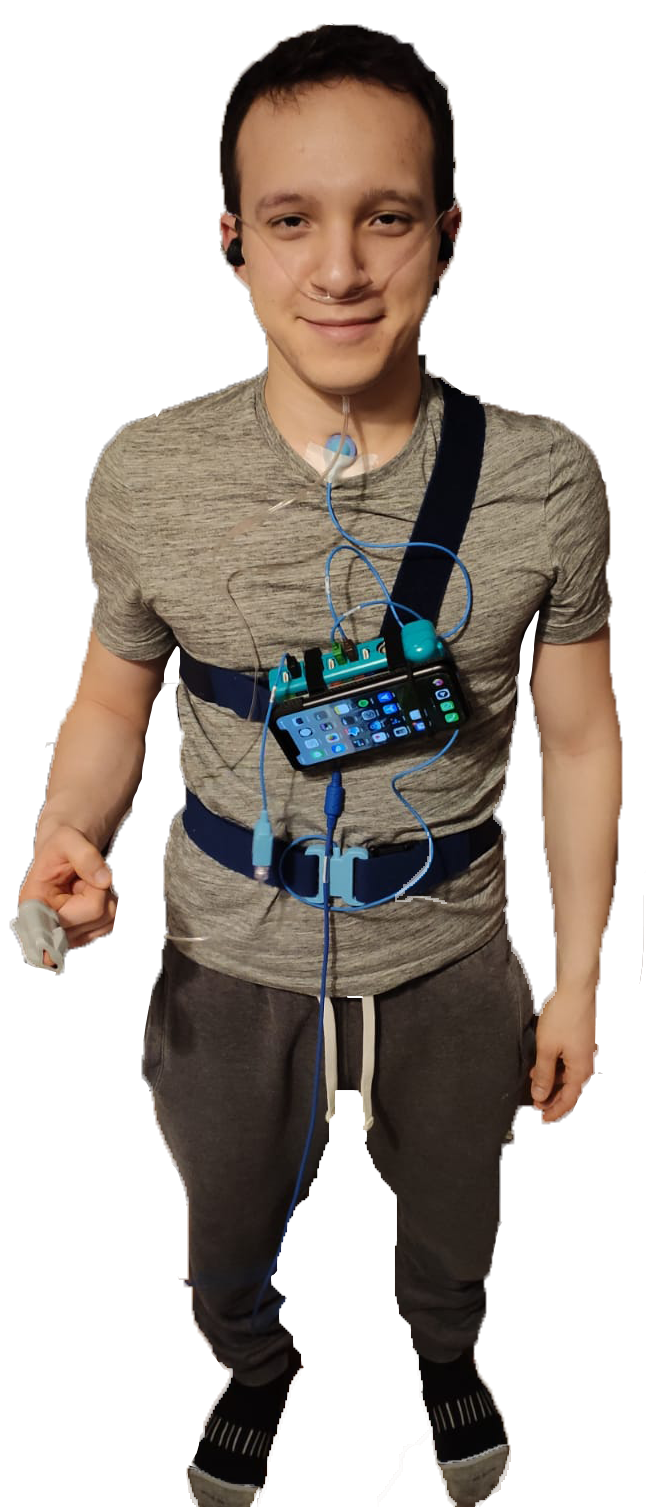
\includegraphics[width=1\textwidth]{study/study_proband_clean2.png}
    \end{subfigure}
    \caption{Darstellung von Beispielprobanden der Nutzerstudie. Das PSG-System wurde mitsamt den Sensoren am Körper angebracht. Zudem wurde das Handy am PSG-System befestigt. Die Person ist nun bereit für die erste Messung.}
    \label{implementation:study:measurement_example}
\end{figure}

Die Evaluation der Ergebnisse beginnt damit, die Daten der eSense Earpods in Fenster (\textit{windows}) einzuteilen.
Auf diese Fenster werden anschließend \textit{Features} berechnet, welche die Grundlage für die Klassifizierung sind.

\newpage 

\section{Gibt es passende Features?}
Die Suche nach passenden Features wird mit dem Python Package \texttt{tsfresh} angegangen.
\texttt{tsfresh} berechnet automatisch Charakteristiken, sowie deren Relevanz anhand eines Zeitintervalls \cite{TsfreshTsfresh12}.
Diese Charakteristiken werden fortan als \textit{Feature} bezeichnet.

Wie in Kapitel \ref{ch:Implementierung:classification_pipeline} bereits erklärt, wird eine Messung in viele sich überlappende Fenster aufgeteilt. 
Eine Messung wird in Fenster der Größe von $5\si{\s}$, bzw. $10\si{\s}$ eingeteilt.
Diese Fenster sind jeweils um $1\si{\s}$ verschoben, d.h. die aneinander grenzenden Fenster überlappen sich um $4\si{\s}$, bzw. $9\si{\s}$.
Nun wird für jedes Fenster eine Featureberechnung ausgeführt, womit durch \texttt{tsfresh} ($\sim$ 6000) Features für jedes Fenster entstehen.
Als Eingabe bekommt \texttt{tsfresh} die Daten der eSense Earpods, also die \textit{x-, y-} und \textit{z}-Achse der Gyroskop und Beschleunigungsdaten, die mit einem Zeitstempel versehen sind. 
Die Abbildung \ref{evaluation:rawPlot} zeigt einen Ausschnitt einer Messung. 
Die in Blau eingefärbte Linie stellt den absoluten Wert aus den Gyroskopdaten der $x$, $y$ und $z$-Achse dar.
In Grün ist das Signal des Drucksensors, direkt unter der Nase befestigt, zu sehen, welches die Atmung repräsentiert.
Der orange markierte Bereich ist jener Bereich, in dem der Proband die Luft angehalten hat. 
Man erkennt bereits, dass die Signale während der Phase des Luftanhaltens wenig Ausschlag in einem Bereich haben.
Wenn der Proband nicht die Luft anhält, erkennt man deutliche Bewegungen der Gyroskopdaten. 

\begin{figure}[ht]
  \centering
  \begin{subfigure}{0.7\textwidth}
      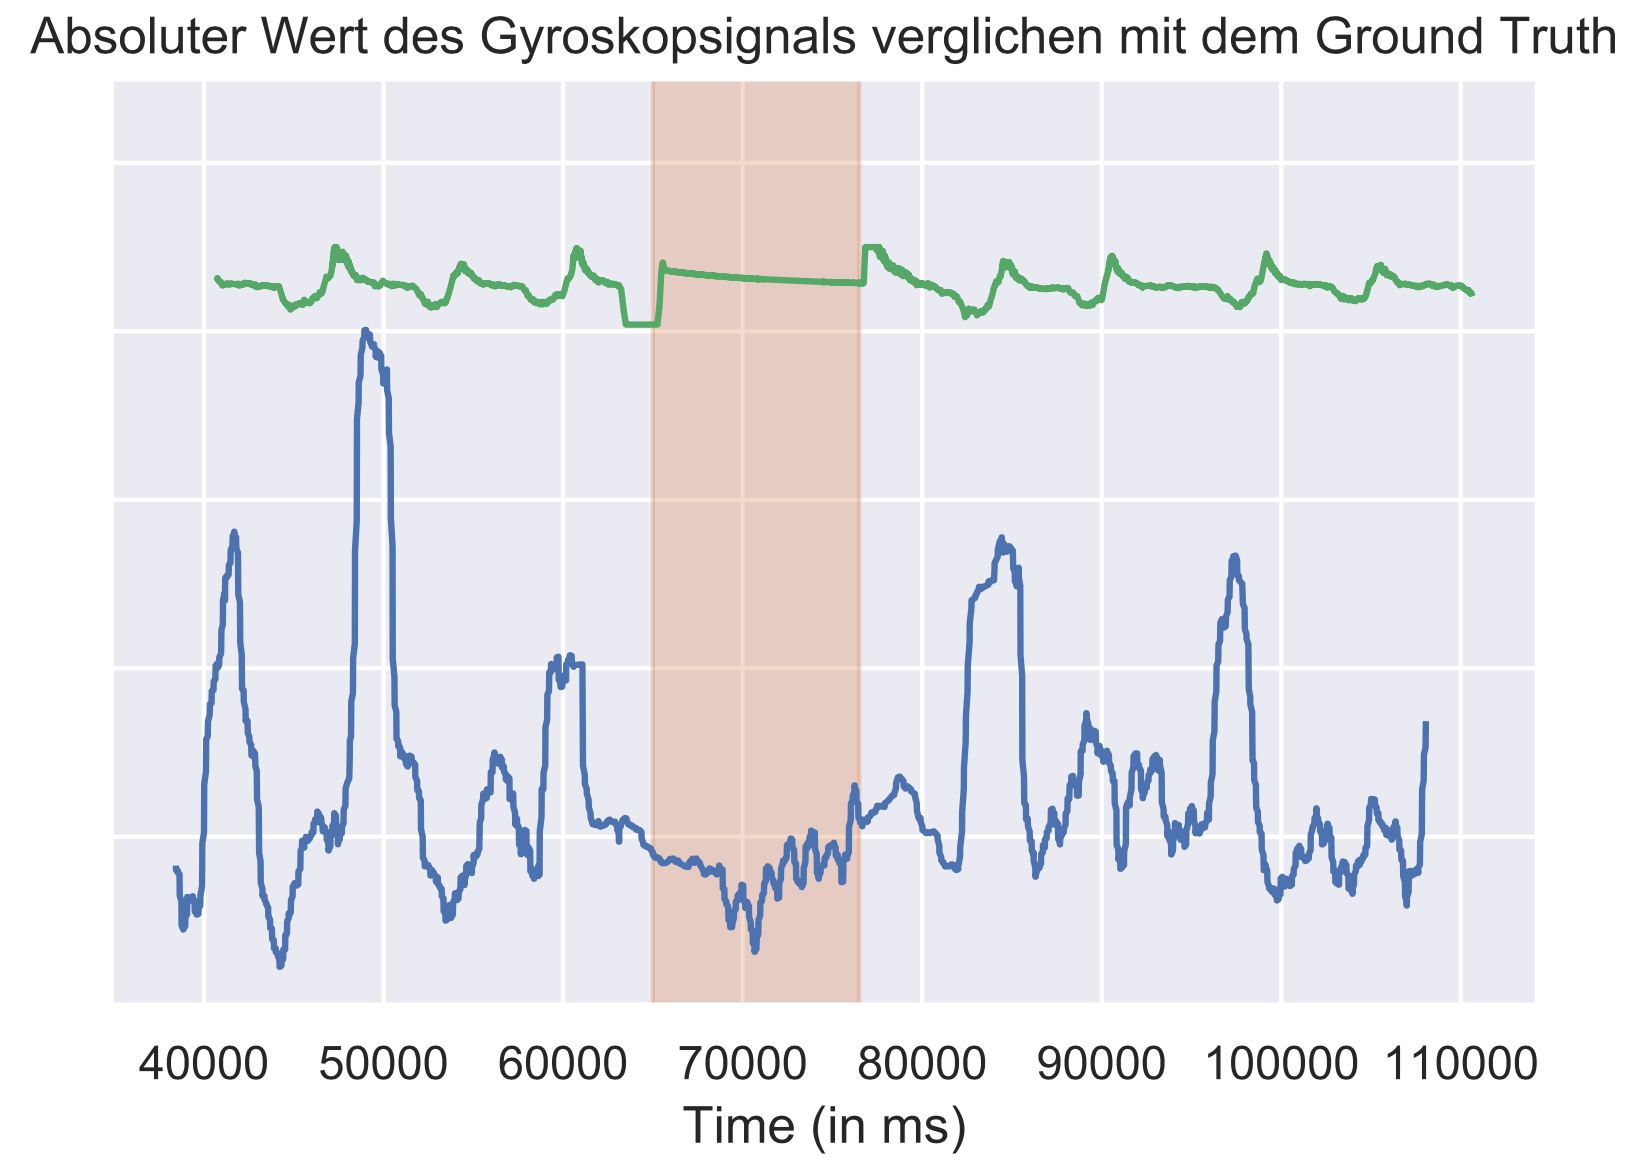
\includegraphics[width=1\textwidth]{data_analyzation/compare_raw_signal_with_flowDr_2.png}
    \end{subfigure}
  \caption{Darstellung des Signals eines Probanden während einer Messung. In Grün ist das Signal des Drucksensors vom PSG-Gerät zu sehen, welcher an der Nase befestigt ist. Zudem ist der absolute Wert, welcher sich aus allen 3 Achsen des Gyroskopsignals berechnen lässt, in blau und das Apnoeereignis in orange zu sehen. Circa zwischen Sekunde 65 und 75 wurde ein Apnoeereignis simuliert. Es ist deutlich zu sehen, dass ein Apnoeereignis auch anhand der IMU-Werte zu erkennen ist. Die Berechnung des absoluten Werts ist $\sqrt{x^2+y^2+z^2}$. Beide Signale wurden normalisiert und so in der y-Achse verschoben, sodass sie vergleichbar sind.}
  \label{evaluation:rawPlot}
\end{figure}

\section{Ablauf der Evaluierung}
Im Kapitel \ref{ch:Implementierung:classification_pipeline} wurde beschrieben, wie die Features berechnet und persistiert wurden. 
Nun sind pro Studienteilnehmer für alle 3 Positionen Features berechnet worden. 
Es sind jeweils die Features für ein Fenster von 5 Sekunden und 10 Sekunden berechnet worden.
Zur Erinnerung: Jede Messung wurde in Fenster der Länge von 5, bzw. 10 Sekunden aufgeteilt, wobei jedes Fenster um eine Sekunde, bzw. 5 und 10 Sekunden verschoben ist.

\subsection{Data Labeling}
Bei Supervised Learning mit Klassifikation müssen die Daten bereits markiert sein, um eine Entscheidung treffen zu können. 
Beim Abspeichern der eSense Daten ist dies bereits geschehen.
Da die Messung genau vorgibt, wann eine Person die Luft anhalten soll und wann nicht, wird diese Information mit einem \textit{Boolean} als zusätzliches Attribut vermerkt.
Da bei der Klassifikation Features anhand der eSense Daten berechnet werden, darf dieses Attribut nicht Teil der Featureberechnung sein.
Bei einem 5 Sekunden Intervall werden circa 250 Einträge, bei einem 10 Sekunden Intervall circa 500 Einträge in eine Featureberechnung zusammenfließen, weshalb eine Markierung dieses Fensters gewählt werden muss.
Ist mehr als die Hälfte der Einträge positiv markiert, gilt das ganze Intervall als positiv markiert.
Dies ist eine essenzielle Entscheidung, da beim Training des Modells nun anhand dieser Markierung entschieden wird, ob ein Intervall einen Atemaussetzer repräsentiert, oder nicht.
Mit einer Grenze von 50\% wurde eine gleichwertige Aufteilung gewählt.
Nun können die Resultate mit den Klassifikatoren verglichen werden.

\subsection{Kreuzvalidierungsverfahren}
\subsubsection{Within Subject (\textit{k-fold cross validation})}
Das erste Kreuzvalidierungsverfahren ist die \textit{k-fold cross validation}.
Bei diesem Verfahren werden alle Daten in $k$ Partitionen aufgeteilt.
Eine Partition wird als Testdatensatz und $k-1$ Partitionen werden als Trainingsdatensatz gewählt \cite{neumannMaschineLearningKIT2020}.
Somit werden alle Personen zu einem Datensatz zusammengefasst und mit der Methode \texttt{test\_train\_split} in Trainingsdaten und Testdaten aufgeteilt.
Hier wird eine Aufteilung von 70\% für die Trainingsdaten und 30\% für die Testdaten gewählt. 
Daraus ergibt sich ein \textit{score}, welcher die mittlere Genauigkeit (\textit{mean accuracy}) auf den gegebenen Testdaten, welche 30\% des Datensatzes sind, angibt.

Die Resultate sind in Abbildung \ref{evaluation:within_subject_results} zu sehen.
Die Tabelle zeigt die Ergebnisse verschiedener Klassifikationsalgorithmen mit verschiedenen Datensätzen.
Pro Klassifikationsalgorithmus wurden alle Positionen, sowie jede Position einzeln betrachtet, d.h jede Position jeder Person.
Jede Kombination aus Klassifikationsalgorithmus und gewähltem Datensatz wurde nun mit den Fenstergrößen von $5\si{\s}$ und $10\si{\s}$ mit einer Verschiebung von $1\si{\s}$ und einer Verschiebung der Fenstergröße evaluiert.
Somit wurden die Fenstergrößen mit und ohne überlappende Fenster getestet.
Die Resultate zeigen, dass der \textit{score} mit überlappenden Fenstern deutlich höher ist.
Dies könnte daran liegen, dass deutlich mehr Fenster pro Datensatz existieren, falls eine Überlappung der aneinanderfolgenden Fenster stattfindet.
Jedoch ist es auch möglich, dass Teile der überlappenden Fenster bereits erkannt und positiv markiert wurden.
Dadurch ist der überlappende Teil eventuell in den Trainingsdaten vorhanden und eine Klassifizierung ist einfach für den Klassifikationsalgorithmus.

\begin{table}[ht]
  \begin{tabular}{cc}
    \begin{minipage}{1\textwidth}
      \begin{center}
          \begin{tabular}{ | l | c | c | c | c | c | }
            \hline
            \textbf{Verfahren} & \textbf{Positionen} & \textbf{Score} & \textbf{Score} & \textbf{Score} & \textbf{Score} \\ 
            & & \textbf{$w=5\si{\s}$} & \textbf{$w=5\si{\s}$} & \textbf{$w=10\si{\s}$} & \textbf{$w=10\si{\s}$} \\
            & & \textbf{$d=1\si{\s}$} & \textbf{$d=5\si{\s}$} & \textbf{$d=1\si{\s}$} & \textbf{$d=10\si{\s}$} \\ \hline
            Random Forest & Alle &  0.87 & 0.74 & 0.89 & 0.71 \\ 
             & Rücken & 0.85 & 0.67 & 0.93 & 0.57 \\
             & Seite  & 0.86 & 0.72 & 0.89 & 0.75 \\
             & Bauch  & 0.90 & 0.85 & 0.92 & 0.66 \\ \hline
            XG Boost  & Alle & 0.88 & 0.70 & 0.92 & 0.76 \\ 
             & Rücken & 0.89 & 0.67 & 0.95 & 0.62 \\
             & Seite  & 0.90 & 0.78 & 0.92 & 0.48 \\
             & Bauch  & 0.90 & 0.75 & 0.95 & 0.63 \\ \hline
            SVM & Alle& 0.54 & 0.48 & 0.65 & 0.42 \\ 
             & Rücken & 0.60 & 0.67 & 0.72 & 0.46 \\
             & Seite  & 0.57 & 0.38 & 0.63 & 0.5 \\
             & Bauch  & 0.61 & 0.41 & 0.67 & 0.4 \\
            \hline
          \end{tabular}
      \end{center}
    \end{minipage}
  \end{tabular}

  \caption{Ergebnisse des Kreuzvalidierungsverfahrens innerhalb eines Subjects mit einer Aufteilung von 70\% Trainings- und 30\% Testdaten. Alle Personen der Nutzerstudie wurden verwendet. $w$ steht für die Fenstergröße, $d$ für die Verschiebung der aneinanderfolgenden Fenster.}
  \label{evaluation:within_subject_results}
\end{table}

\subsubsection{Leave One Subject Out (LOSO)}
Neben dem k-fachen Kreuzvalidierungsverfahren wird das \textit{Leave One Subject Out} (\textit{LOSO}) Kreuzvalidierungsverfahren hinzugezogen. 
Hierbei wird ein Modell anhand der Daten der Studienteilnehmer trainiert, jedoch wird ein Datensatz eines Studienteilnehmers ausgelassen. 
Dieser eine Datensatz wird schließlich verwendet, um eine Vorhersage anhand der Trainingsdaten zu treffen, ohne durch interne Trainingsdaten optimiert sein zu können.
Im Folgenden wurde das LOSO Kreuzvalidierungsverfahren mit den beiden Klassifikationsalgorithmen \textit{Random Forest} und \textit{XGBoost} durchgeführt. 
Es wurde jede Person einmal ausgelassen und auf den Trainingsdatensatz vorhergesagt, welcher diese Person nicht enthält. 
Somit entstehen 7 Resultate, von denen nun der Mittelwert gebildet wurde.
Die Resultate sind in den Abbildungen \ref{evaluation:random_forest_loso:person6} und \ref{evaluation:xgboost_loso:person6} beispielhaft an Person 6 dargestellt.
Im Anhang sind weitere Abbildungen anderer Personen zu finden.
Die Abbildungen listen die Häufigkeit der Vorhersagen für jede einzelne Sekunde auf. 
Da eine Sekunde aufgrund der überlappenden Fenster in mehreren Fenstern vorkommt, summieren sich die Vorhersagen pro Sekunde maximal auf die Fenstergröße.
Zu Erkennen ist, dass die Fenstergröße von $10\si{\s}$ deutlich bessere Ergebnisse liefert, als eine Fenstergröße von $5\si{\s}$. 
XGBoost neigt bei einer Fenstergröße von $5\si{\s}$ zum Overfitting, ebenso wie Random Forest. 
Alle Ergebnisse des LOSO Kreuzvalidierungsverfahrens sind im \textit{Precision} und \textit{Recall} der unterliegenden Tabelle der Beispiele bei Person 6 mit dem Mittelwert zusammengetragen worden. 
Zu sehen ist, dass XGBoost bessere Ergebnisse liefert als Random Forest.
% \todo{schreibe darüber, was die ergebnisse von LOSO aussagen} \newline
Des Weiteren, um mögliche Positionsabhängigkeiten zu erkennen, wurde dasselbe erneut evaluiert, jedoch nur mit den einzelnen Positionsdaten der jeweiligen Person. 
In der Tabelle \ref{evaluation:loso_classification_results} sind die Resultate zu sehen.
%\todo{schreibe darüber, was die ergebnisse der einzelnen personen aussagen}

\subsection{Relevante Features}
Jede Klassifikation ergab ein Resultat, welches durch einzelne Features entschieden wurde. 
Das Python-Framework \texttt{scikit-learn} beinhaltet \texttt{feature\_importances\_} und zeigt die Relevanz der einzelnen Features in einem Plot.
Um einen kleinen Überblick zu bekommen, welche Features entscheidend für die Evaluation waren, sind nun einige aufgelistet:
\begin{itemize}
    \item \texttt{gyroZ partial autocorrelation}
    \item \texttt{gytoX fft coefficient}
    \item \texttt{gyroX agg autocorrelation}
    \item \texttt{accY autocorrelation}
    \item \texttt{gyroY change quantiles }
    \item \texttt{gyroZ fft coefficient}
\end{itemize}
Diese Features wurden mittels \texttt{tsfresh} berechnet und waren bei der Klassifikation des Kreuzvalidierungsverfahrens entscheidened \cite{TsfreshTsfresh12}.

Die partielle Autokorrelationfunktion (\texttt{partial autocorrelation}) beschreibt die Abhänigkeit zwischen den Werten der Zeitreihen. 
Zudem wird ein zeitlicher linearer Zusammenhang der verschiedenen Werte gemessen.
Somit haben sich die Werte in diesem Fenster zwischen den Werten weniger verändert und ähneln somit eher den positiv markierten Trainingsdaten.

Die \textit{Schnelle Fourier-Transformation} berechnet effizient die diskrete Fourier-Transformation.
Damit können zeitdiskrete Signale in Frequenzanteile zerlegt werden. 
Es wird aus einer Darstellung, bestehend aus einem Zeit- und Abtastwert in einer Darstellung, bestehend aus einem Frequenzanteil, einer Amplitude und einer Phase überführt.
Die Funktion \texttt{fft\_coefficient} in \texttt{tsfresh} berechnet die Fourier Koeffizienten einer eindimensionalen diskreten Fouriertransformation für eine reale Eingabe mit dem Algorithmus der Fast-Fourier-Transformation:
\[A_k = \sum_{m=0}^{n-1} a_m \exp ^ {-2\pi i \frac{mk}{n}}, \hspace{1cm} k = 0,\dots,n-1\]
Die bei der Apnoephase geringe Amplitude ist hier erkennbar und detektierbar, womit eine Klassifikation ermöglicht wird.

Die Aggregation \texttt{agg\_autocorrelation} berechnet den Wert der Autokorrelationsfunktion $f_{agg}$ (beispielsweise die Varianz oder den Mittelwert) über die Autokorrelation $R(l)$ für die verschiedenen Fenster. 
\[R(l) = \frac{1}{(n-l)\sigma ^2} \sum_{t=1}^{n-l} (X_t - \mu) (X_{t+l} - \mu)\]
$X_i$ sind hierbei  die Werte der Zeitreihe (\textit{Timeseries}), $n$ deren Länge. 
$\sigma$ und $\mu$ sind Schätzwerte für die Varianz und den Mittelwert.

Ein weiteres Feature, welches ausschlaggebend für die Klassifikation ist, ist der Wechsel der Quantilwerte (\texttt{change\_quantiles}).
Pro Fenster wird ein $q_l$ niedriges Quantil und ein $q_h$ hohes Quantil berechnet. 
Anschließend wird der durchschnittliche, absolute Wert der aufeinanderfolgenden Änderungen der Reihe $x$ innerhalb dieser Quantile berechnet.
Dadurch werden starke Veränderungen deutlich und zeigen, dass in diesem Fenster kein Apnoe stattfindet. 

\subsection{Vorverarbeitung durch einen Tiefpassfilter}
Als weiterer Versuch wurde ein Tiefpassfilter auf die Gyroskop- und Beschleunigungsdaten angewandt. 
Im Anschluss wurden Features mittels \texttt{tsfresh} auf jedem Fenster berechnet.
Da \texttt{tsfresh} ebenfalls Tiefpassfilter zur Featureberechnung nutzt, ergaben sich mit \textit{Random Forest} und \textit{XGBoost} schlechtere Resultate.
Dies ist darauf zurückzuführen, dass durch den Tiefpassfilter Informationen verloren gehen, welche in der Featureberechnung anschließend nicht mehr zur Verfügung stehen. 

%%%%%%%%%%%%%%%%%%%        RANDOM FOREST 5 sec %%%%%%%%%%%%%%%%%%%%%%%%%%%%%%%%%
\begin{figure}[ht]
  \textbf{Random Forest ($w=5\si{\s}$, $d=1\si{\s}$)}
    \centering
    \begin{subfigure}{1\textwidth}
        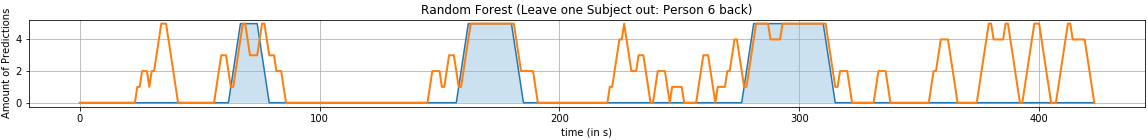
\includegraphics[width=1\textwidth]{evaluation/loso_5sec/random_forest_loso/Random Forest (Leave one Subject out: Person 6 back).png}
        %\caption{Resultate der Person 6 auf dem Rücken liegend.}
      \end{subfigure}
      \begin{subfigure}{1\textwidth}
        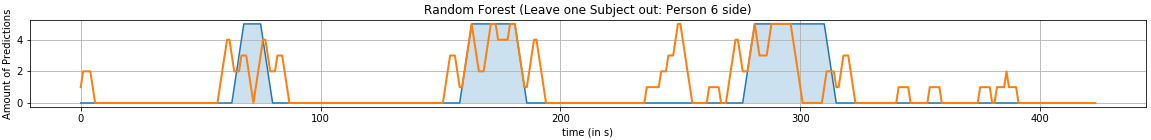
\includegraphics[width=1\textwidth]{evaluation/loso_5sec/random_forest_loso/Random Forest (Leave one Subject out: Person 6 side).png}
        %\caption{Resultate der Person 6 auf der Seite liegend.}
      \end{subfigure}
      \begin{subfigure}{1\textwidth}
        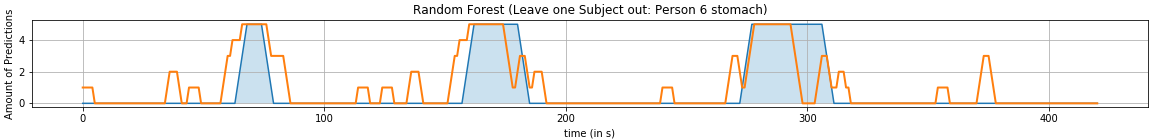
\includegraphics[width=1\textwidth]{evaluation/loso_5sec/random_forest_loso/Random Forest (Leave one Subject out: Person 6 stomach).png}
        %\caption{Resultate der Person 6 auf dem Bauch liegend.}
    \end{subfigure}
    \begin{subfigure}{1\textwidth}
        \begin{center}
            \begin{tabular}{ | l | c | c | r | }
              \hline
               & precision & recall & f1-score\\ \hline
              0 & 0.92 & 0.75 & 0.81 \\ \hline
              1 & 0.75 & 0.67 & 0.47 \\
              \hline
            \end{tabular}
        \end{center}
        \caption{Random Forest mit dem Kreuzvalidierungsverfahren (LOSO): Die Tabelle zeigt den Mittelwert aller Vorhersagen der einzelnen Personen.}
        \label{implementation:app:screenshots:user_studies_information}
    \end{subfigure}
    \newline
    \vspace*{1 cm}
    \newline
    \textbf{Random Forest ($w=10\si{\s}$, $d=1\si{\s}$)}
    \begin{subfigure}{1\textwidth}
      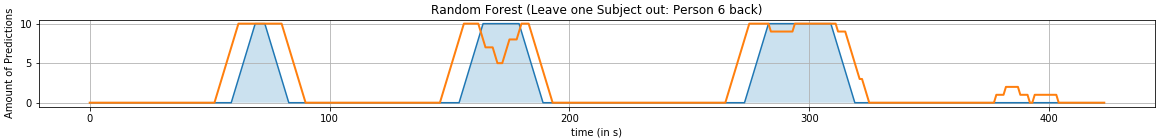
\includegraphics[width=1\textwidth]{evaluation/loso_10sec/random_forest_loso/Random Forest (Leave one Subject out: Person 6 back).png}
      %\caption{Resultate der Person 6 auf dem Rücken liegend.}
    \end{subfigure}
    \begin{subfigure}{1\textwidth}
      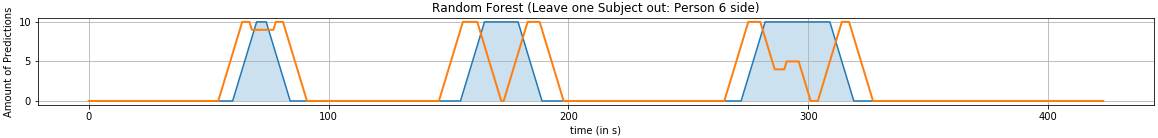
\includegraphics[width=1\textwidth]{evaluation/loso_10sec/random_forest_loso/Random Forest (Leave one Subject out: Person 6 side).png}
      %\caption{Resultate der Person 6 auf der Seite liegend.}
    \end{subfigure}
    \begin{subfigure}{1\textwidth}
      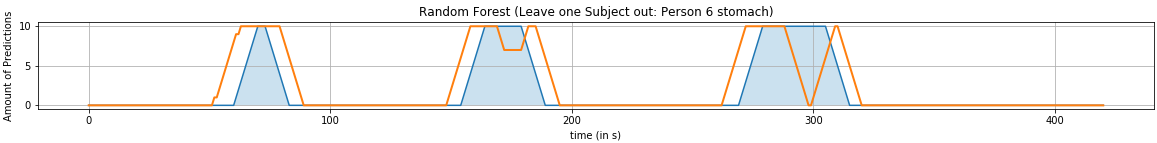
\includegraphics[width=1\textwidth]{evaluation/loso_10sec/random_forest_loso/Random Forest (Leave one Subject out: Person 6 stomach).png}
      %\caption{Resultate der Person 6 auf dem Bauch liegend.}
  \end{subfigure}

  \begin{subfigure}{1\textwidth}
      \begin{center}
          \begin{tabular}{ | l | c | c | r | }
            \hline
             & precision & recall & f1-score\\ \hline
            0 & 0.92 & 0.77 & 0.83\\ \hline
            1 & 0.77 & 0.67 & 0.5\\
            \hline
          \end{tabular}
      \end{center}
      \caption{Random Forest mit dem Kreuzvalidierungsverfahren (LOSO): Die Tabelle zeigt den Mittelwert aller Vorhersagen der einzelnen Personen.}
      \label{implementation:app:screenshots:user_studies_information}
  \end{subfigure}
    \caption{Das Kreuzvalidierungsverfahren (LOSO) mit dem Klassifikationsalgorithmus Random Forest. Das Modell wurde auf allen Personen, exklusive einer Person, trainiert. Auf alle Positionen dieser einen Person wurde eine Vorhersage getroffen. Beim Beispiel hier sind die Resultate von Person 6 zu sehen. Die blauen Bereiche sind die, in denen die Luft angehalten wurde, die orange Kurve zeigt die Vorhersage ($w=$ Fenstergröße, $d=$ Verschiebung der Fenster).}
\label{evaluation:random_forest_loso:person6}
\end{figure}

%%%%%%%%%%%%%%%%%%%        XG BOOST 5 sec %%%%%%%%%%%%%%%%%%%%%%%%%%%%%%%%%

\begin{figure}[ht]
  \textbf{XG Boost ($w=5\si{\s}$, $d=1\si{\s}$)}
    \centering
    \begin{subfigure}{1\textwidth}
        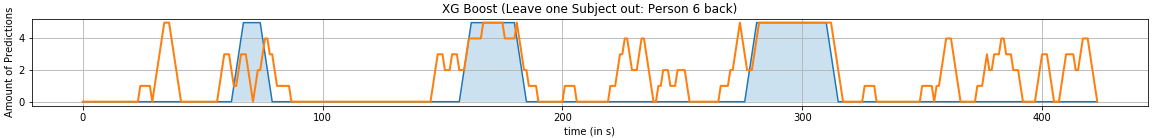
\includegraphics[width=1\textwidth]{evaluation/loso_5sec/xg_boost_loso/XG Boost (Leave one Subject out: Person 6 back).png}
        %\caption{Resultate der Person 6 auf dem Rücken liegend.}
      \end{subfigure}
      \begin{subfigure}{1\textwidth}
        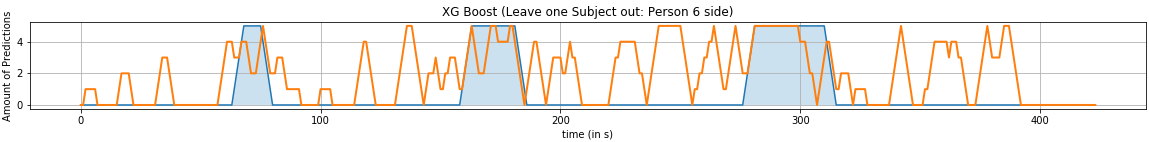
\includegraphics[width=1\textwidth]{evaluation/loso_5sec/xg_boost_loso/XG Boost (Leave one Subject out: Person 6 side).png}
        %\caption{Resultate der Person 6 auf der Seite liegend.}
      \end{subfigure}
      \begin{subfigure}{1\textwidth}
        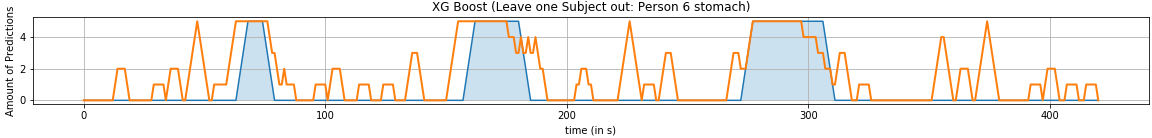
\includegraphics[width=1\textwidth]{evaluation/loso_5sec/xg_boost_loso/XG Boost (Leave one Subject out: Person 6 stomach).png}
        %\caption{Resultate der Person 6 auf dem Bauch liegend.}
    \end{subfigure}

    \begin{subfigure}{1\textwidth}
        \begin{center}
            \begin{tabular}{ | l | c | c | r | }
              \hline
               & precision & recall & f1-score \\ \hline
              0 & 0.93 & 0.71 & 0.79 \\ \hline
              1 & 0.72 & 0.69 & 0.47 \\
              \hline
            \end{tabular}
        \end{center}
        \caption{XGBoost mit dem Kreuzvalidierungsverfahren (LOSO): Die Tabelle zeigt den Mittelwert aller Vorhersagen der einzelnen Personen.}
        \label{implementation:app:screenshots:user_studies_information}
    \end{subfigure}
    \newline
    \vspace*{1 cm}
    \newline
    \textbf{XG Boost ($w=10\si{\s}$, $d=1\si{\s}$)}
    \begin{subfigure}{1\textwidth}
      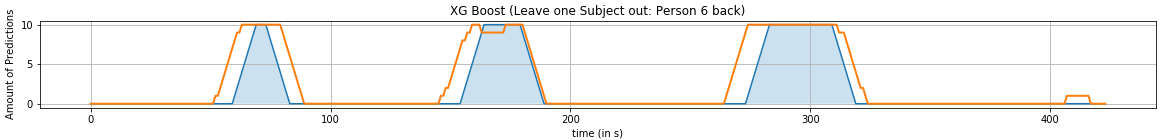
\includegraphics[width=1\textwidth]{evaluation/loso_10sec/xg_boost_loso/XG Boost (Leave one Subject out: Person 6 back).png}
      %\caption{Klassifikationsresultate der Person 6. Die Messung wurde auf dem Rücken liegend durchgeführt.}
    \end{subfigure}
    \begin{subfigure}{1\textwidth}
      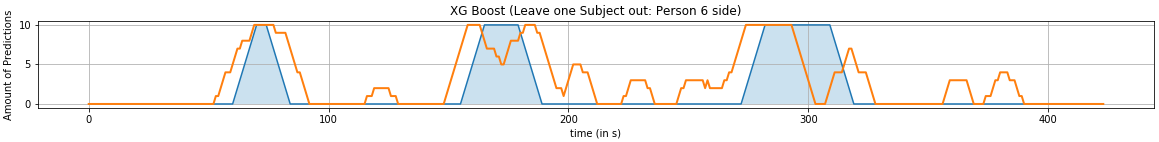
\includegraphics[width=1\textwidth]{evaluation/loso_10sec/xg_boost_loso/XG Boost (Leave one Subject out: Person 6 side).png}
      %\caption{Klassifikationsresultate der Person 6. Die Messung wurde auf der Seite liegend durchgeführt.}
    \end{subfigure}
    \begin{subfigure}{1\textwidth}
      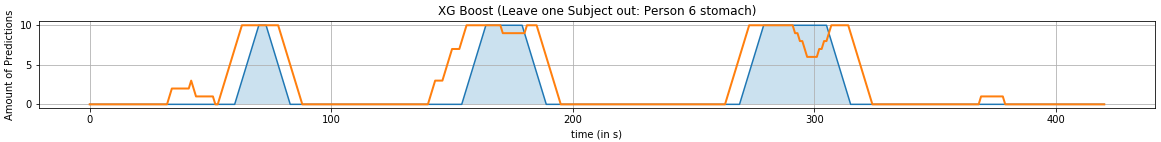
\includegraphics[width=1\textwidth]{evaluation/loso_10sec/xg_boost_loso/XG Boost (Leave one Subject out: Person 6 stomach).png}
      %\caption{Klassifikationsresultate der Person 6. Die Messung wurde auf dem Bauch liegend durchgeführt.}
  \end{subfigure}

  \begin{subfigure}{1\textwidth}
      \begin{center}
          \begin{tabular}{ | l | c | c | r | }
            \hline
             & precision & recall & f1-score \\ \hline
            0 & 0.93 & 0.74 & 0.8 \\ \hline
            1 & 0.74 & 0.75 & 0.5 \\
            \hline
          \end{tabular}
      \end{center}
      \caption{XGBoost mit dem Kreuzvalidierungsverfahren (LOSO): Die Tabelle zeigt den Mittelwert aller Vorhersagen der einzelnen Personen.}
      \label{implementation:app:screenshots:user_studies_information}
  \end{subfigure}
    \caption{Das Kreuzvalidierungsverfahren (LOSO) mit dem Klassifikationsalgorithmus XG Boost: Das Modell wurde auf allen Personen, exklusive einer Person trainiert. Auf alle Positionen dieser einen Person wurde eine Vorhersage getroffen. Am Beispiel hier sind die Resultate von Person 6 zu sehen. Die blauen Bereiche sind die, in denen die Luft angehalten wurde, die orange Kurve zeigt die Vorhersage ($w=$ Fenstergröße, $d=$ Verschiebung der Fenster).}
\label{evaluation:xgboost_loso:person6}
\end{figure}

%%%%%%%%%%%%%%%%%%%        Position based results  5 sec %%%%%%%%%%%%%%%%%%%%%%%%%%%%%%%%%
\begin{table}
  \begin{tabular}{cc}
    \begin{minipage}{1\linewidth}
      \begin{center}
          \begin{tabular}{ | l | c | c | c | c | c | r | }
            \hline
            Klassifikation & Fenstergröße & Position & & precision & recall & f1-score \\ \hline
            Random Forest & 5s & Seite & 0 & 0.86 & 0.76 & 0.81 \\ 
                          &    &       & 1 & 0.76 & 0.57 & 0.48 \\ \hline
                          &    & Rücken& 0 & 0.90 & 0.79 & 0.83 \\ 
                          &    &       & 1 & 0.83 & 0.52 & 0.39 \\ \hline
                          &    & Bauch & 0 & 0.92 & 0.72 & 0.70 \\ 
                          &    &       & 1 & 0.72 & 0.69 & 0.52 \\ \hline
            \hline
            XG Boost & 5s & Seite & 0 & 0.91 & 0.67 & 0.71 \\
                     &    &       & 1 & 0.67 & 0.61 & 0.35 \\ \hline
                     &    & Rücken& 0 & 0.90 & 0.74 & 0.80 \\ 
                     &    &       & 1 & 0.75 & 0.57 & 0.38 \\ \hline
                     &    & Bauch & 0 & 0.94 & 0.71 & 0.74 \\ 
                     &    &       & 1 & 0.71 & 0.72 & 0.55 \\ \hline
            \hline
            Random Forest & 10s & Seite & 0 & 0.89 & 0.77 & 0.83 \\ 
                          &     &       & 1 & 0.80 & 0.67 & 0.5 \\ \hline
                          &     & Rücken& 0 & 0.89 & 0.83 & 0.85 \\
                          &     &       & 1 & 0.82 & 0.52 & 0.41 \\ \hline
                          &     & Bauch & 0 & 0.93 & 0.71 & 0.74 \\
                          &     &       & 1 & 0.71 & 0.70 & 0.49 \\ \hline
            \hline
            XGBoost & 10s & Seite & 0 & 0.90 & 0.78 & 0.78 \\
                    &     &       & 1 & 0.78 & 0.71 & 0.47 \\ \hline
                    &     & Rücken& 0 & 0.90 & 0.85 & 0.86 \\
                    &     &       & 1 & 0.85 & 0.50 & 0.44 \\ \hline
                    &     & Bauch & 0 & 0.94 & 0.72 & 0.75 \\
                    &     &       & 1 & 0.72 & 0.70 & 0.53 \\ \hline
          \end{tabular}
          \smallskip
      \end{center}
      %\label{evaluation:5s:random_forest_loso_side}
  \end{minipage} 
    
  \end{tabular}
  \caption{Zu sehen sind die Klassifikationsergebnisse mit dem Kreuzvalidierungsverfahren bei einer Fenstergröße von 5 bzw. 10 Sekunden, welche um 1 Sekunde verschoben wurden. Es wurde immer eine Person beim Trainieren des Modells ausgelassen. Für diese Person wurde anschließend eine Vorhersage getroffen. Jede Person wurde einmel in dem Modell außen vorgelassen und für dieses Modell vorhergesagt. Das zu sehende Resultat ist der Mittelwert aller Resultate des Kreuzvalidierungsverfahrens der einzelnen Positionen.}
  \label{evaluation:loso_classification_results}  
\end{table}        % Evaluierung
%% zusammenf.tex
%% $Id: zusammenf.tex 4 2005-10-10 20:51:21Z bless $
%%

\chapter{Zusammenfassung und Future Work}
\label{ch:FutureWork}
%% ==============================
%
  % Future Work
\include{src/summary}   % Zusammenfassung und Ausblick
\chapter{Anhang}
\label{ch:anhang}
Im Anhang sind weitere Resultate des Kreuzvalidierungsverfahrens {\glqq Leave One Subject Out\grqq} aufgelistet.
Es wurde zuerst die Resultate der Person 5, 7 und 8 aufgelistet, wobei hier alle Positionen im Modell mittrainiert wurden und eine Vorhersage auf jede Position getroffen wurde.
In orange sind die Vorhersagen der Fenster für jede Sekunde aufaddiert, in blau sind die Markierungen der Fenster aufaddiert.

Es ist erkennbar, dass bei Person 5 kaum Bereiche als positiv markiert vorhergesagt wurden, in denen kein Apnoeereignis simuliert wurde.
jedoch wurden nicht alle Fenster der Apnoeereignisse als solche klassifiziert.

Bei Person 7 ist klar zu erkennen, dass eine Fenstergröße von 10 Sekunden deutlich bessere Resultate liefert im Vergleich zu einer Fenstergröße von 5 Sekunden.
Hier ist die Variation der Vorhersage von Proband zu Proband gut zu sehen.
Person 8 zeigt jedoch auch, dass die Ergebnisse bei einer Fenstergröße von 10s auch nicht immer gut sind.

%% ==============================
%

%%%%%      PERSON 5 LOSO %%%%%%%%%%%%%%%%%%%%%%%
\begin{figure}
    \textbf{Person 5: Random Forest ($w=5\si{\s}$, $d=1\si{\s}$)}
      \centering
      \begin{subfigure}{1\textwidth}
          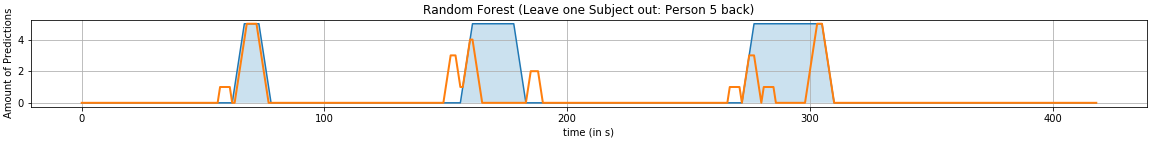
\includegraphics[width=1\textwidth]{evaluation/loso_5sec/random_forest_loso/Random Forest (Leave one Subject out: Person 5 back).png}
          %\caption{Resultate der Person 6 auf dem Rücken liegend.}
        \end{subfigure}
        \begin{subfigure}{1\textwidth}
          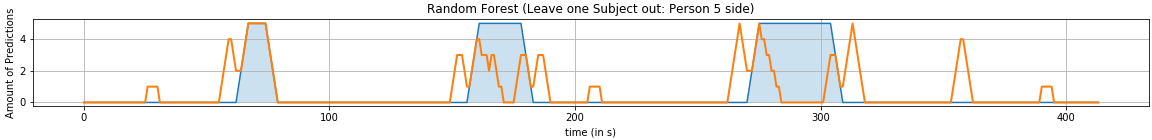
\includegraphics[width=1\textwidth]{evaluation/loso_5sec/random_forest_loso/Random Forest (Leave one Subject out: Person 5 side).png}
          %\caption{Resultate der Person 6 auf der Seite liegend.}
        \end{subfigure}
        \begin{subfigure}{1\textwidth}
          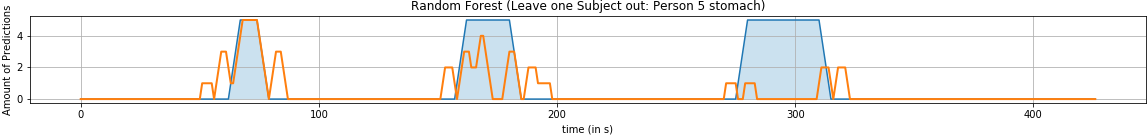
\includegraphics[width=1\textwidth]{evaluation/loso_5sec/random_forest_loso/Random Forest (Leave one Subject out: Person 5 stomach).png}
          %\caption{Resultate der Person 6 auf dem Bauch liegend.}
      \end{subfigure}
        \textbf{Person 5: Random Forest ($w=10\si{\s}$, $d=1\si{\s}$)}
      \centering
      \begin{subfigure}{1\textwidth}
          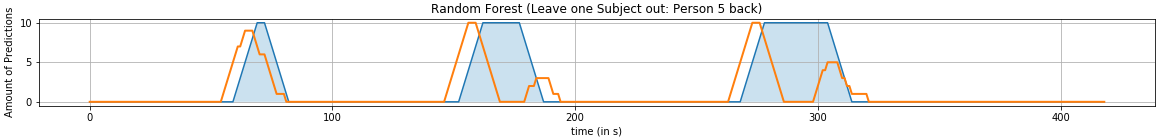
\includegraphics[width=1\textwidth]{evaluation/loso_10sec/random_forest_loso/Random Forest (Leave one Subject out: Person 5 back).png}
          %\caption{Resultate der Person 6 auf dem Rücken liegend.}
        \end{subfigure}
        \begin{subfigure}{1\textwidth}
          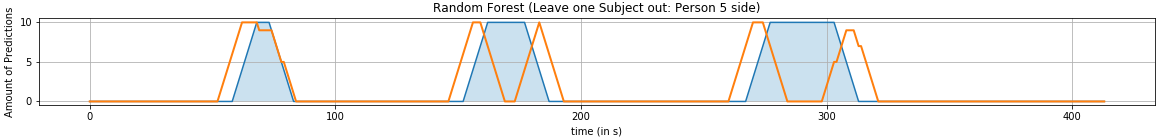
\includegraphics[width=1\textwidth]{evaluation/loso_10sec/random_forest_loso/Random Forest (Leave one Subject out: Person 5 side).png}
          %\caption{Resultate der Person 6 auf der Seite liegend.}
        \end{subfigure}
        \begin{subfigure}{1\textwidth}
          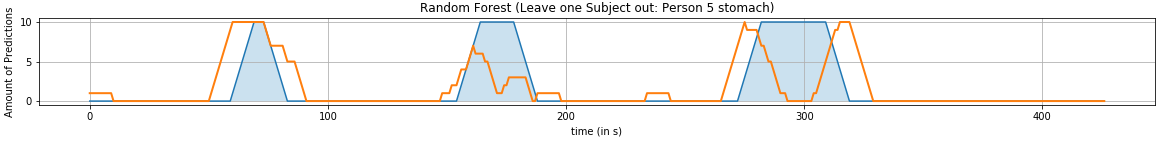
\includegraphics[width=1\textwidth]{evaluation/loso_10sec/random_forest_loso/Random Forest (Leave one Subject out: Person 5 stomach).png}
          %\caption{Resultate der Person 6 auf dem Bauch liegend.}
      \end{subfigure}
  
      %\caption{Das Kreuzvalidierungsverfahren (LOSO) mit dem Klassifikationsalgorithmus XG Boost. Das Modell wurde auf allen Personen, exklusive einer Person trainiert und auf alle Positionen dieser einen Person wurde eine Vorhersage getroffen. Am Beispiel hier sind die Resultate von Person 6 zu sehen. Die blauen Bereiche sind die, in denen die Luft angehalten wurde, die orangene Kurve ist die Vorhersage. ($w=$ Fenstergröße, $d=$ Verschiebung der Fenster)}
      \label{evaluation:random_forest_loso:person5}
\end{figure}
\begin{figure}
    \textbf{Person 5: XG Boost ($w=5\si{\s}$, $d=1\si{\s}$)}
      \centering
      \begin{subfigure}{1\textwidth}
          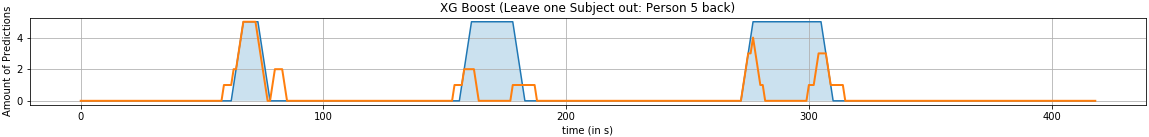
\includegraphics[width=1\textwidth]{evaluation/loso_5sec/xg_boost_loso/XG Boost (Leave one Subject out: Person 5 back).png}
          %\caption{Resultate der Person 6 auf dem Rücken liegend.}
        \end{subfigure}
        \begin{subfigure}{1\textwidth}
          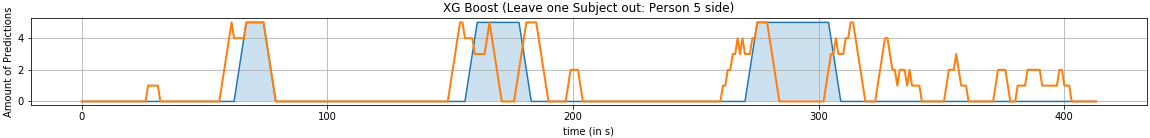
\includegraphics[width=1\textwidth]{evaluation/loso_5sec/xg_boost_loso/XG Boost (Leave one Subject out: Person 5 side).png}
          %\caption{Resultate der Person 6 auf der Seite liegend.}
        \end{subfigure}
        \begin{subfigure}{1\textwidth}
          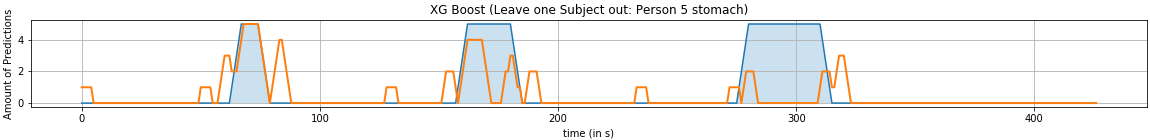
\includegraphics[width=1\textwidth]{evaluation/loso_5sec/xg_boost_loso/XG Boost (Leave one Subject out: Person 5 stomach).png}
          %\caption{Resultate der Person 6 auf dem Bauch liegend.}
      \end{subfigure}
        \textbf{Person 5: XG Boost ($w=10\si{\s}$, $d=1\si{\s}$)}
      \centering
      \begin{subfigure}{1\textwidth}
          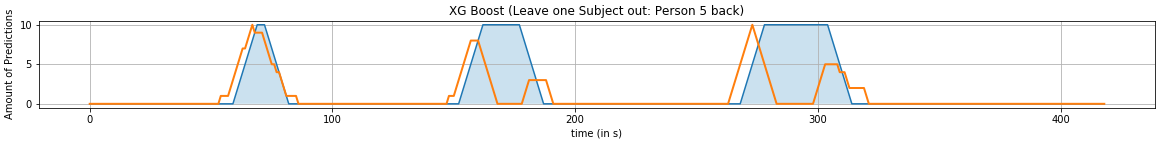
\includegraphics[width=1\textwidth]{evaluation/loso_10sec/xg_boost_loso/XG Boost (Leave one Subject out: Person 5 back).png}
          %\caption{Resultate der Person 6 auf dem Rücken liegend.}
        \end{subfigure}
        \begin{subfigure}{1\textwidth}
          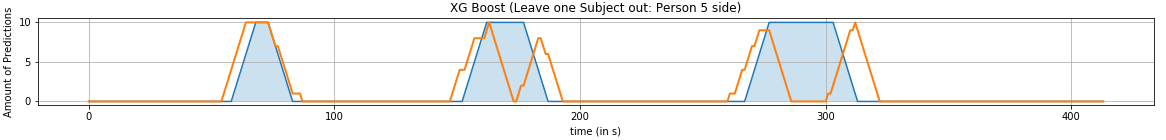
\includegraphics[width=1\textwidth]{evaluation/loso_10sec/xg_boost_loso/XG Boost (Leave one Subject out: Person 5 side).png}
          %\caption{Resultate der Person 6 auf der Seite liegend.}
        \end{subfigure}
        \begin{subfigure}{1\textwidth}
          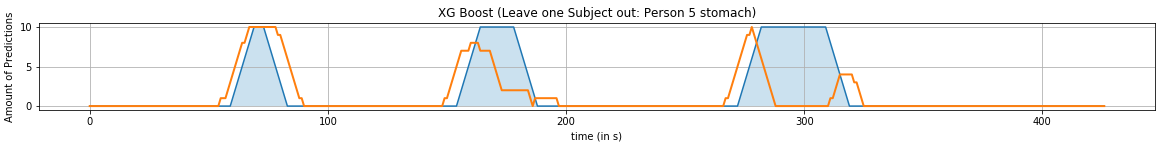
\includegraphics[width=1\textwidth]{evaluation/loso_10sec/xg_boost_loso/XG Boost (Leave one Subject out: Person 5 stomach).png}
          %\caption{Resultate der Person 6 auf dem Bauch liegend.}
      \end{subfigure}
  
      %\caption{Das Kreuzvalidierungsverfahren (LOSO) mit dem Klassifikationsalgorithmus XG Boost. Das Modell wurde auf allen Personen, exklusive einer Person trainiert und auf alle Positionen dieser einen Person wurde eine Vorhersage getroffen. Am Beispiel hier sind die Resultate von Person 6 zu sehen. Die blauen Bereiche sind die, in denen die Luft angehalten wurde, die orangene Kurve ist die Vorhersage. ($w=$ Fenstergröße, $d=$ Verschiebung der Fenster)}
      \label{evaluation:xgboost_loso:person5}
\end{figure}

%%%%%      PERSON 5 LOSO %%%%%%%%%%%%%%%%%%%%%%%
\begin{figure}
    \textbf{Person 7: Random Forest ($w=5\si{\s}$, $d=1\si{\s}$)}
      \centering
      \begin{subfigure}{1\textwidth}
          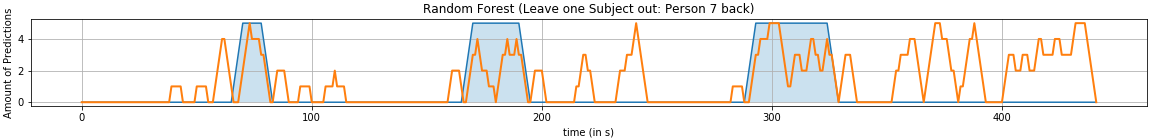
\includegraphics[width=1\textwidth]{evaluation/loso_5sec/random_forest_loso/Random Forest (Leave one Subject out: Person 7 back).png}
          %\caption{Resultate der Person 6 auf dem Rücken liegend.}
        \end{subfigure}
        \begin{subfigure}{1\textwidth}
          \includegraphics[width=1\textwidth]{evaluation/loso_5sec/random_forest_loso/Random Forest (Leave one Subject out: Person 7 side).png}
          %\caption{Resultate der Person 6 auf der Seite liegend.}
        \end{subfigure}
        \begin{subfigure}{1\textwidth}
          \includegraphics[width=1\textwidth]{evaluation/loso_5sec/random_forest_loso/Random Forest (Leave one Subject out: Person 7 stomach).png}
          %\caption{Resultate der Person 6 auf dem Bauch liegend.}
      \end{subfigure}
        \textbf{Person 7: Random Forest ($w=10\si{\s}$, $d=1\si{\s}$)}
      \centering
      \begin{subfigure}{1\textwidth}
          \includegraphics[width=1\textwidth]{evaluation/loso_10sec/random_forest_loso/Random Forest (Leave one Subject out: Person 7 back).png}
          %\caption{Resultate der Person 6 auf dem Rücken liegend.}
        \end{subfigure}
        \begin{subfigure}{1\textwidth}
          \includegraphics[width=1\textwidth]{evaluation/loso_10sec/random_forest_loso/Random Forest (Leave one Subject out: Person 7 side).png}
          %\caption{Resultate der Person 6 auf der Seite liegend.}
        \end{subfigure}
        \begin{subfigure}{1\textwidth}
          \includegraphics[width=1\textwidth]{evaluation/loso_10sec/random_forest_loso/Random Forest (Leave one Subject out: Person 7 stomach).png}
          %\caption{Resultate der Person 6 auf dem Bauch liegend.}
      \end{subfigure}
  
      %\caption{Das Kreuzvalidierungsverfahren (LOSO) mit dem Klassifikationsalgorithmus XG Boost. Das Modell wurde auf allen Personen, exklusive einer Person trainiert und auf alle Positionen dieser einen Person wurde eine Vorhersage getroffen. Am Beispiel hier sind die Resultate von Person 6 zu sehen. Die blauen Bereiche sind die, in denen die Luft angehalten wurde, die orangene Kurve ist die Vorhersage. ($w=$ Fenstergröße, $d=$ Verschiebung der Fenster)}
      \label{evaluation:random_forest_loso:person7}
\end{figure}
\begin{figure}
    \textbf{Person 7: XG Boost ($w=5\si{\s}$, $d=1\si{\s}$)}
      \centering
      \begin{subfigure}{1\textwidth}
          \includegraphics[width=1\textwidth]{evaluation/loso_5sec/xg_boost_loso/XG Boost (Leave one Subject out: Person 7 back).png}
          %\caption{Resultate der Person 6 auf dem Rücken liegend.}
        \end{subfigure}
        \begin{subfigure}{1\textwidth}
          \includegraphics[width=1\textwidth]{evaluation/loso_5sec/xg_boost_loso/XG Boost (Leave one Subject out: Person 7 side).png}
          %\caption{Resultate der Person 6 auf der Seite liegend.}
        \end{subfigure}
        \begin{subfigure}{1\textwidth}
          \includegraphics[width=1\textwidth]{evaluation/loso_5sec/xg_boost_loso/XG Boost (Leave one Subject out: Person 7 stomach).png}
          %\caption{Resultate der Person 6 auf dem Bauch liegend.}
      \end{subfigure}
        \textbf{Person 7: XG Boost ($w=10\si{\s}$, $d=1\si{\s}$)}
      \centering
      \begin{subfigure}{1\textwidth}
          \includegraphics[width=1\textwidth]{evaluation/loso_10sec/xg_boost_loso/XG Boost (Leave one Subject out: Person 7 back).png}
          %\caption{Resultate der Person 6 auf dem Rücken liegend.}
        \end{subfigure}
        \begin{subfigure}{1\textwidth}
          \includegraphics[width=1\textwidth]{evaluation/loso_10sec/xg_boost_loso/XG Boost (Leave one Subject out: Person 7 side).png}
          %\caption{Resultate der Person 6 auf der Seite liegend.}
        \end{subfigure}
        \begin{subfigure}{1\textwidth}
          \includegraphics[width=1\textwidth]{evaluation/loso_10sec/xg_boost_loso/XG Boost (Leave one Subject out: Person 7 stomach).png}
          %\caption{Resultate der Person 6 auf dem Bauch liegend.}
      \end{subfigure}
  
      %\caption{Das Kreuzvalidierungsverfahren (LOSO) mit dem Klassifikationsalgorithmus XG Boost. Das Modell wurde auf allen Personen, exklusive einer Person trainiert und auf alle Positionen dieser einen Person wurde eine Vorhersage getroffen. Am Beispiel hier sind die Resultate von Person 6 zu sehen. Die blauen Bereiche sind die, in denen die Luft angehalten wurde, die orangene Kurve ist die Vorhersage. ($w=$ Fenstergröße, $d=$ Verschiebung der Fenster)}
      \label{evaluation:xgboost_loso:person7}
\end{figure}

%%%%%      PERSON 8 LOSO %%%%%%%%%%%%%%%%%%%%%%%
\begin{figure}
    \textbf{Person 8: Random Forest ($w=5\si{\s}$, $d=1\si{\s}$)}
      \centering
      \begin{subfigure}{1\textwidth}
          \includegraphics[width=1\textwidth]{evaluation/loso_5sec/random_forest_loso/Random Forest (Leave one Subject out: Person 8 back).png}
          %\caption{Resultate der Person 6 auf dem Rücken liegend.}
        \end{subfigure}
        \begin{subfigure}{1\textwidth}
          \includegraphics[width=1\textwidth]{evaluation/loso_5sec/random_forest_loso/Random Forest (Leave one Subject out: Person 8 side).png}
          %\caption{Resultate der Person 6 auf der Seite liegend.}
        \end{subfigure}
        \begin{subfigure}{1\textwidth}
          \includegraphics[width=1\textwidth]{evaluation/loso_5sec/random_forest_loso/Random Forest (Leave one Subject out: Person 8 stomach).png}
          %\caption{Resultate der Person 6 auf dem Bauch liegend.}
      \end{subfigure}
        \textbf{Person 8: Random Forest ($w=10\si{\s}$, $d=1\si{\s}$)}
      \centering
      \begin{subfigure}{1\textwidth}
          \includegraphics[width=1\textwidth]{evaluation/loso_10sec/random_forest_loso/Random Forest (Leave one Subject out: Person 8 back).png}
          %\caption{Resultate der Person 6 auf dem Rücken liegend.}
        \end{subfigure}
        \begin{subfigure}{1\textwidth}
          \includegraphics[width=1\textwidth]{evaluation/loso_10sec/random_forest_loso/Random Forest (Leave one Subject out: Person 8 side).png}
          %\caption{Resultate der Person 6 auf der Seite liegend.}
        \end{subfigure}
        \begin{subfigure}{1\textwidth}
          \includegraphics[width=1\textwidth]{evaluation/loso_10sec/random_forest_loso/Random Forest (Leave one Subject out: Person 8 stomach).png}
          %\caption{Resultate der Person 6 auf dem Bauch liegend.}
      \end{subfigure}
  
      %\caption{Das Kreuzvalidierungsverfahren (LOSO) mit dem Klassifikationsalgorithmus XG Boost. Das Modell wurde auf allen Personen, exklusive einer Person trainiert und auf alle Positionen dieser einen Person wurde eine Vorhersage getroffen. Am Beispiel hier sind die Resultate von Person 6 zu sehen. Die blauen Bereiche sind die, in denen die Luft angehalten wurde, die orangene Kurve ist die Vorhersage. ($w=$ Fenstergröße, $d=$ Verschiebung der Fenster)}
      \label{evaluation:random_forest_loso:person8}
\end{figure}
\begin{figure}
    \textbf{Person 8: XG Boost ($w=5\si{\s}$, $d=1\si{\s}$)}
      \centering
      \begin{subfigure}{1\textwidth}
          \includegraphics[width=1\textwidth]{evaluation/loso_5sec/xg_boost_loso/XG Boost (Leave one Subject out: Person 8 back).png}
          %\caption{Resultate der Person 6 auf dem Rücken liegend.}
        \end{subfigure}
        \begin{subfigure}{1\textwidth}
          \includegraphics[width=1\textwidth]{evaluation/loso_5sec/xg_boost_loso/XG Boost (Leave one Subject out: Person 8 side).png}
          %\caption{Resultate der Person 6 auf der Seite liegend.}
        \end{subfigure}
        \begin{subfigure}{1\textwidth}
          \includegraphics[width=1\textwidth]{evaluation/loso_5sec/xg_boost_loso/XG Boost (Leave one Subject out: Person 8 stomach).png}
          %\caption{Resultate der Person 6 auf dem Bauch liegend.}
      \end{subfigure}
        \textbf{Person 8: XG Boost ($w=10\si{\s}$, $d=1\si{\s}$)}
      \centering
      \begin{subfigure}{1\textwidth}
          \includegraphics[width=1\textwidth]{evaluation/loso_10sec/xg_boost_loso/XG Boost (Leave one Subject out: Person 8 back).png}
          %\caption{Resultate der Person 6 auf dem Rücken liegend.}
        \end{subfigure}
        \begin{subfigure}{1\textwidth}
          \includegraphics[width=1\textwidth]{evaluation/loso_10sec/xg_boost_loso/XG Boost (Leave one Subject out: Person 8 side).png}
          %\caption{Resultate der Person 6 auf der Seite liegend.}
        \end{subfigure}
        \begin{subfigure}{1\textwidth}
          \includegraphics[width=1\textwidth]{evaluation/loso_10sec/xg_boost_loso/XG Boost (Leave one Subject out: Person 8 stomach).png}
          %\caption{Resultate der Person 6 auf dem Bauch liegend.}
      \end{subfigure}
  
      %\caption{Das Kreuzvalidierungsverfahren (LOSO) mit dem Klassifikationsalgorithmus XG Boost. Das Modell wurde auf allen Personen, exklusive einer Person trainiert und auf alle Positionen dieser einen Person wurde eine Vorhersage getroffen. Am Beispiel hier sind die Resultate von Person 6 zu sehen. Die blauen Bereiche sind die, in denen die Luft angehalten wurde, die orangene Kurve ist die Vorhersage. ($w=$ Fenstergröße, $d=$ Verschiebung der Fenster)}
      \label{evaluation:xgboost_loso:person8}
\end{figure}

%%%%%      PERSON 5 LOSO %%%%%%%%%%%%%%%%%%%%%%%
\begin{figure}
    \textbf{Person 5 (nur einzelne Positionen): Random Forest ($w=5\si{\s}$, $d=1\si{\s}$)}
      \centering
      \begin{subfigure}{1\textwidth}
          \includegraphics[width=1\textwidth]{evaluation/loso_5sec/random_forest_loso_back_prediction/Random Forest (Leave one Subject out, only back data: Person 5).png}
          %\caption{Resultate der Person 6 auf dem Rücken liegend.}
        \end{subfigure}
        \begin{subfigure}{1\textwidth}
          \includegraphics[width=1\textwidth]{evaluation/loso_5sec/random_forest_loso_side_prediction/Random Forest (Leave one Subject out, only side data: Person 5).png}
          %\caption{Resultate der Person 6 auf der Seite liegend.}
        \end{subfigure}
        \begin{subfigure}{1\textwidth}
          \includegraphics[width=1\textwidth]{evaluation/loso_5sec/random_forest_loso_stomach_prediction/Random Forest (Leave one Subject out, only stomach data: Person 5).png}
          %\caption{Resultate der Person 6 auf dem Bauch liegend.}
      \end{subfigure}
        \textbf{Person 5 (nur einzelne Positionen): XGBoost ($w=5\si{\s}$, $d=1\si{\s}$)}
      \centering
      \begin{subfigure}{1\textwidth}
          \includegraphics[width=1\textwidth]{evaluation/loso_5sec/xg_boost_loso_back_prediction/XG Boost (Leave one Subject out, only back data: Person 5).png}
          %\caption{Resultate der Person 6 auf dem Rücken liegend.}
        \end{subfigure}
        \begin{subfigure}{1\textwidth}
            \includegraphics[width=1\textwidth]{evaluation/loso_5sec/xg_boost_loso_side_prediction/XG Boost (Leave one Subject out, only side data: Person 5).png}
          %\caption{Resultate der Person 6 auf der Seite liegend.}
        \end{subfigure}
        \begin{subfigure}{1\textwidth}
            \includegraphics[width=1\textwidth]{evaluation/loso_5sec/xg_boost_loso_stomach_prediction/XG Boost (Leave one Subject out, only stomach data: Person 5).png}
          %\caption{Resultate der Person 6 auf dem Bauch liegend.}
      \end{subfigure}
  
      %\caption{Das Kreuzvalidierungsverfahren (LOSO) mit dem Klassifikationsalgorithmus XG Boost. Das Modell wurde auf allen Personen, exklusive einer Person trainiert und auf alle Positionen dieser einen Person wurde eine Vorhersage getroffen. Am Beispiel hier sind die Resultate von Person 6 zu sehen. Die blauen Bereiche sind die, in denen die Luft angehalten wurde, die orangene Kurve ist die Vorhersage. ($w=$ Fenstergröße, $d=$ Verschiebung der Fenster)}
      \label{evaluation:random_forest:person5}
\end{figure}
\begin{figure}
    \textbf{Person 5 (nur einzelne Positionen): Random Forest ($w=10\si{\s}$, $d=1\si{\s}$)}
      \centering
      \begin{subfigure}{1\textwidth}
          \includegraphics[width=1\textwidth]{evaluation/loso_10sec/random_forest_loso_back_prediction/Random Forest (Leave one Subject out, only back data: Person 5).png}
          %\caption{Resultate der Person 6 auf dem Rücken liegend.}
        \end{subfigure}
        \begin{subfigure}{1\textwidth}
          \includegraphics[width=1\textwidth]{evaluation/loso_10sec/random_forest_loso_side_prediction/Random Forest (Leave one Subject out, only side data: Person 5).png}
          %\caption{Resultate der Person 6 auf der Seite liegend.}
        \end{subfigure}
        \begin{subfigure}{1\textwidth}
          \includegraphics[width=1\textwidth]{evaluation/loso_10sec/random_forest_loso_stomach_prediction/Random Forest (Leave one Subject out, only stomach data: Person 5).png}
          %\caption{Resultate der Person 6 auf dem Bauch liegend.}
      \end{subfigure}
        \textbf{Person 5 (nur einzelne Positionen): XGBoost ($w=10\si{\s}$, $d=1\si{\s}$)}
      \centering
      \begin{subfigure}{1\textwidth}
          \includegraphics[width=1\textwidth]{evaluation/loso_10sec/xg_boost_loso_back_prediction/XG Boost (Leave one Subject out, only back data: Person 5).png}
          %\caption{Resultate der Person 6 auf dem Rücken liegend.}
        \end{subfigure}
        \begin{subfigure}{1\textwidth}
            \includegraphics[width=1\textwidth]{evaluation/loso_10sec/xg_boost_loso_side_prediction/XG Boost (Leave one Subject out, only side data: Person 5).png}
          %\caption{Resultate der Person 6 auf der Seite liegend.}
        \end{subfigure}
        \begin{subfigure}{1\textwidth}
            \includegraphics[width=1\textwidth]{evaluation/loso_10sec/xg_boost_loso_stomach_prediction/XG Boost (Leave one Subject out, only stomach data: Person 5).png}
          %\caption{Resultate der Person 6 auf dem Bauch liegend.}
      \end{subfigure}
  
      %\caption{Das Kreuzvalidierungsverfahren (LOSO) mit dem Klassifikationsalgorithmus XG Boost. Das Modell wurde auf allen Personen, exklusive einer Person trainiert und auf alle Positionen dieser einen Person wurde eine Vorhersage getroffen. Am Beispiel hier sind die Resultate von Person 6 zu sehen. Die blauen Bereiche sind die, in denen die Luft angehalten wurde, die orangene Kurve ist die Vorhersage. ($w=$ Fenstergröße, $d=$ Verschiebung der Fenster)}
      \label{evaluation:xgboost:person5}
\end{figure}   % Anhang

%% ++++++++++++++++++++++++++++++++++++++++++
%% Anhang
%% ++++++++++++++++++++++++++++++++++++++++++

\appendix
%\include{anhang_a}
%\include{anhang_b}

%% ++++++++++++++++++++++++++++++++++++++++++
%% Literatur
%% ++++++++++++++++++++++++++++++++++++++++++
%  mit dem Befehl \nocite werden auch nicht 
%  zitierte Referenzen abgedruckt
\cleardoublepage
\phantomsection
\addcontentsline{toc}{chapter}{\bibname}
%%
%\nocite{*} % nur angeben, wenn auch nicht im Text zitierte Quellen 
           % erscheinen sollen
%\bibliographystyle{itmabbrv} % mit abgekürzten Vornamen der Autoren
%\bibliographystyle{gerplain} % abbrvnat unsrtnat
% spezielle Zitierstile: Labels mit vier Buchstaben und Jahreszahl
% \bibliographystyle{itmalpha}  % ausgeschriebene Vornamen der Autoren
\printbibliography
%% ++++++++++++++++++++++++++++++++++++++++++
%% Index
%% ++++++++++++++++++++++++++++++++++++++++++
\ifnotdraft{
\cleardoublepage
\phantomsection
\printindex            % Index, Stichwortverzeichnis
}
\end{document}
%% end of file

